\chapter{Resultados}


\section{Seleção dos métodos matemáticos}

Nesta seção é evidenciado os resultados  das simulações dos Experts em linguagem MQL4 (produto da implementação dos métodos matemáticos) através de relatórios e gráficos gerados pela plataforma MetaTrader.

\subsection{Implementação dos métodos matemáticos}

Os métodos de Correlação Linear, Média Móvel, Mínimos Quadrados, Estocástico e Fibonacci foram implementados em linguagem MQL4 e assim foi construído um \textit{expert} para cada método. Esses produtos de software receberam os nomes, respectivamente, CorrelacaoPearson.mql, MediaMovel.mql, MinimosQuadrados.mql, Estocastico.mql e Fibonacci.mql. Cada \textit{expert} encontra-se no apêndice D - Experts para Experimento.

\subsubsection{Simulação do método de Correlação Linear}

O \textit{expert} CorrelacaoPearson.mql obteve o percentual de negociações com lucros de 56.86\% no período de Agosto de 2012 a Agosto de2013. Nesse período, o \textit{expert} teve um lucro de 1981.60 USD. No período de Agosto de 2013 a Agosto de 2014, o percentual de negociações com lucros foi de 55.56\%  e obteve-se o lucro de 1119.05 USD. 
Os relatórios completos das simulações podem ser visualizados nas Figuras \ref{protocoloCorrelacao} e \ref{protocoloCorrelacao2}.

\begin{figure}[H]
\centering
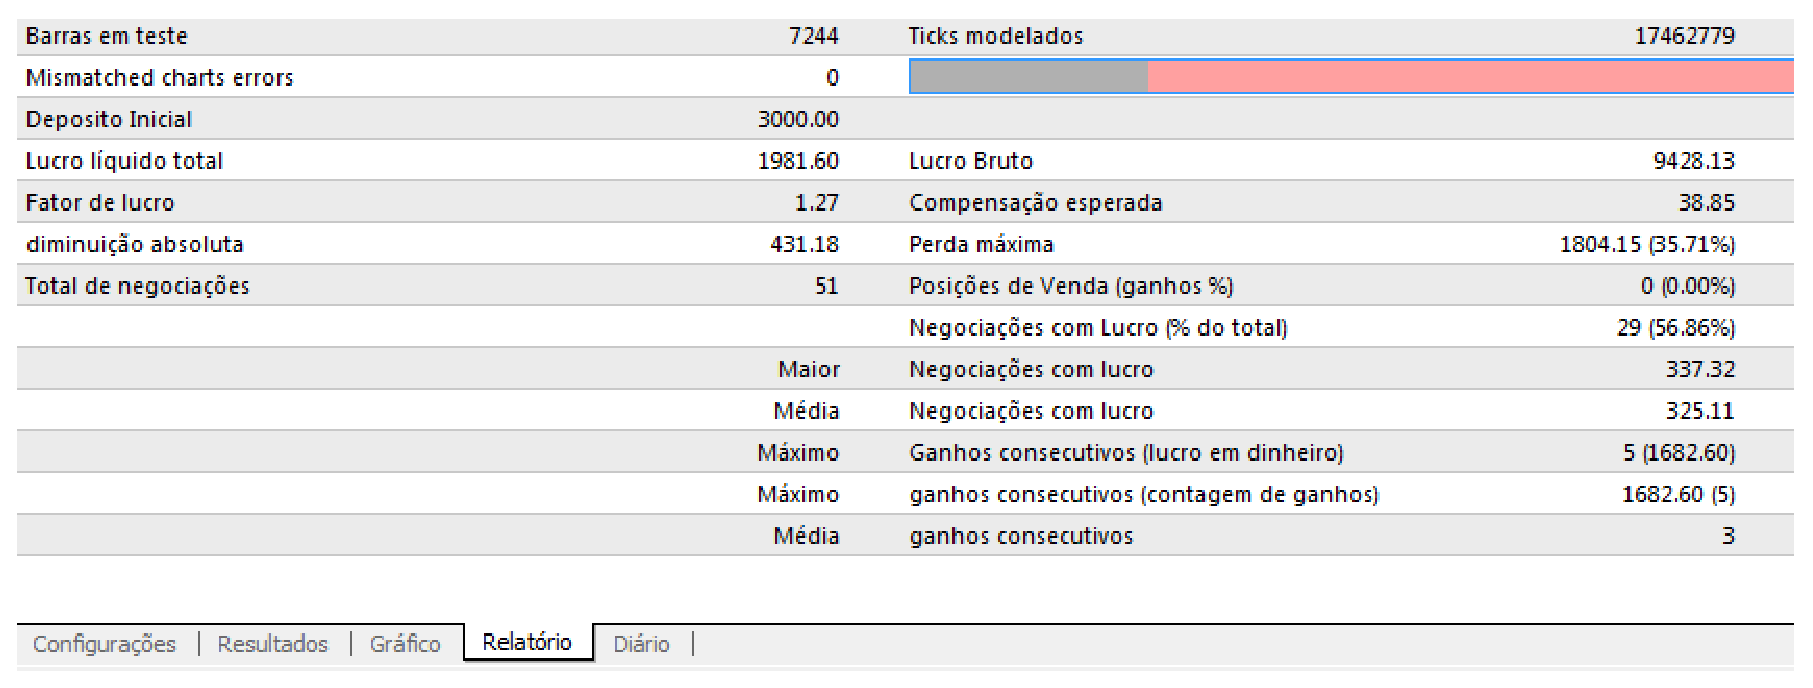
\includegraphics[width=0.9\textwidth]{figuras/protocoloCorrelacao}
\caption{Relatório de simulação no período de Agosto de 2012 a Agosto de 2013 do \textit{expert} CorrelacaoPearson.mql}
\label{protocoloCorrelacao}
\end{figure}

\begin{figure}[H]
\centering

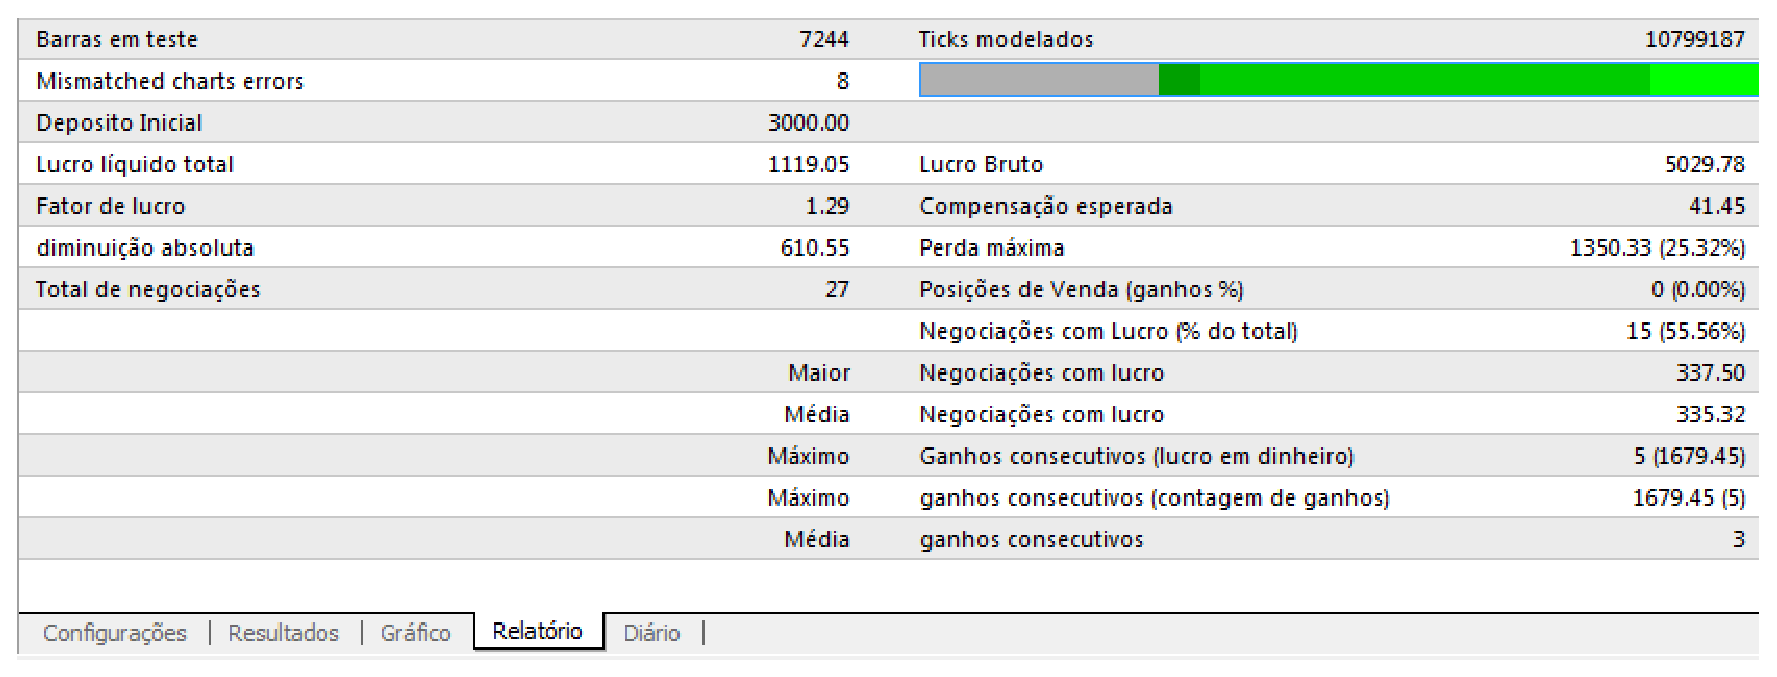
\includegraphics[width=0.9\textwidth]{figuras/protocoloCorrelacao2}
\caption{Relatório de simulação no período de Agosto de 2013 a Agosto de 2014 do\textit{expert} CorrelacaoPearson.mql}
\label{protocoloCorrelacao2}
\end{figure}

Foram gerados os gráficos de simulação de 2012 a 2013 e de 2013 a 2014. É possível perceber que o método de Correlação de Pearson, perde dinheiro em alguns períodos, mas os ganhos são superiores as perdas.

\begin{figure}[H]
\centering
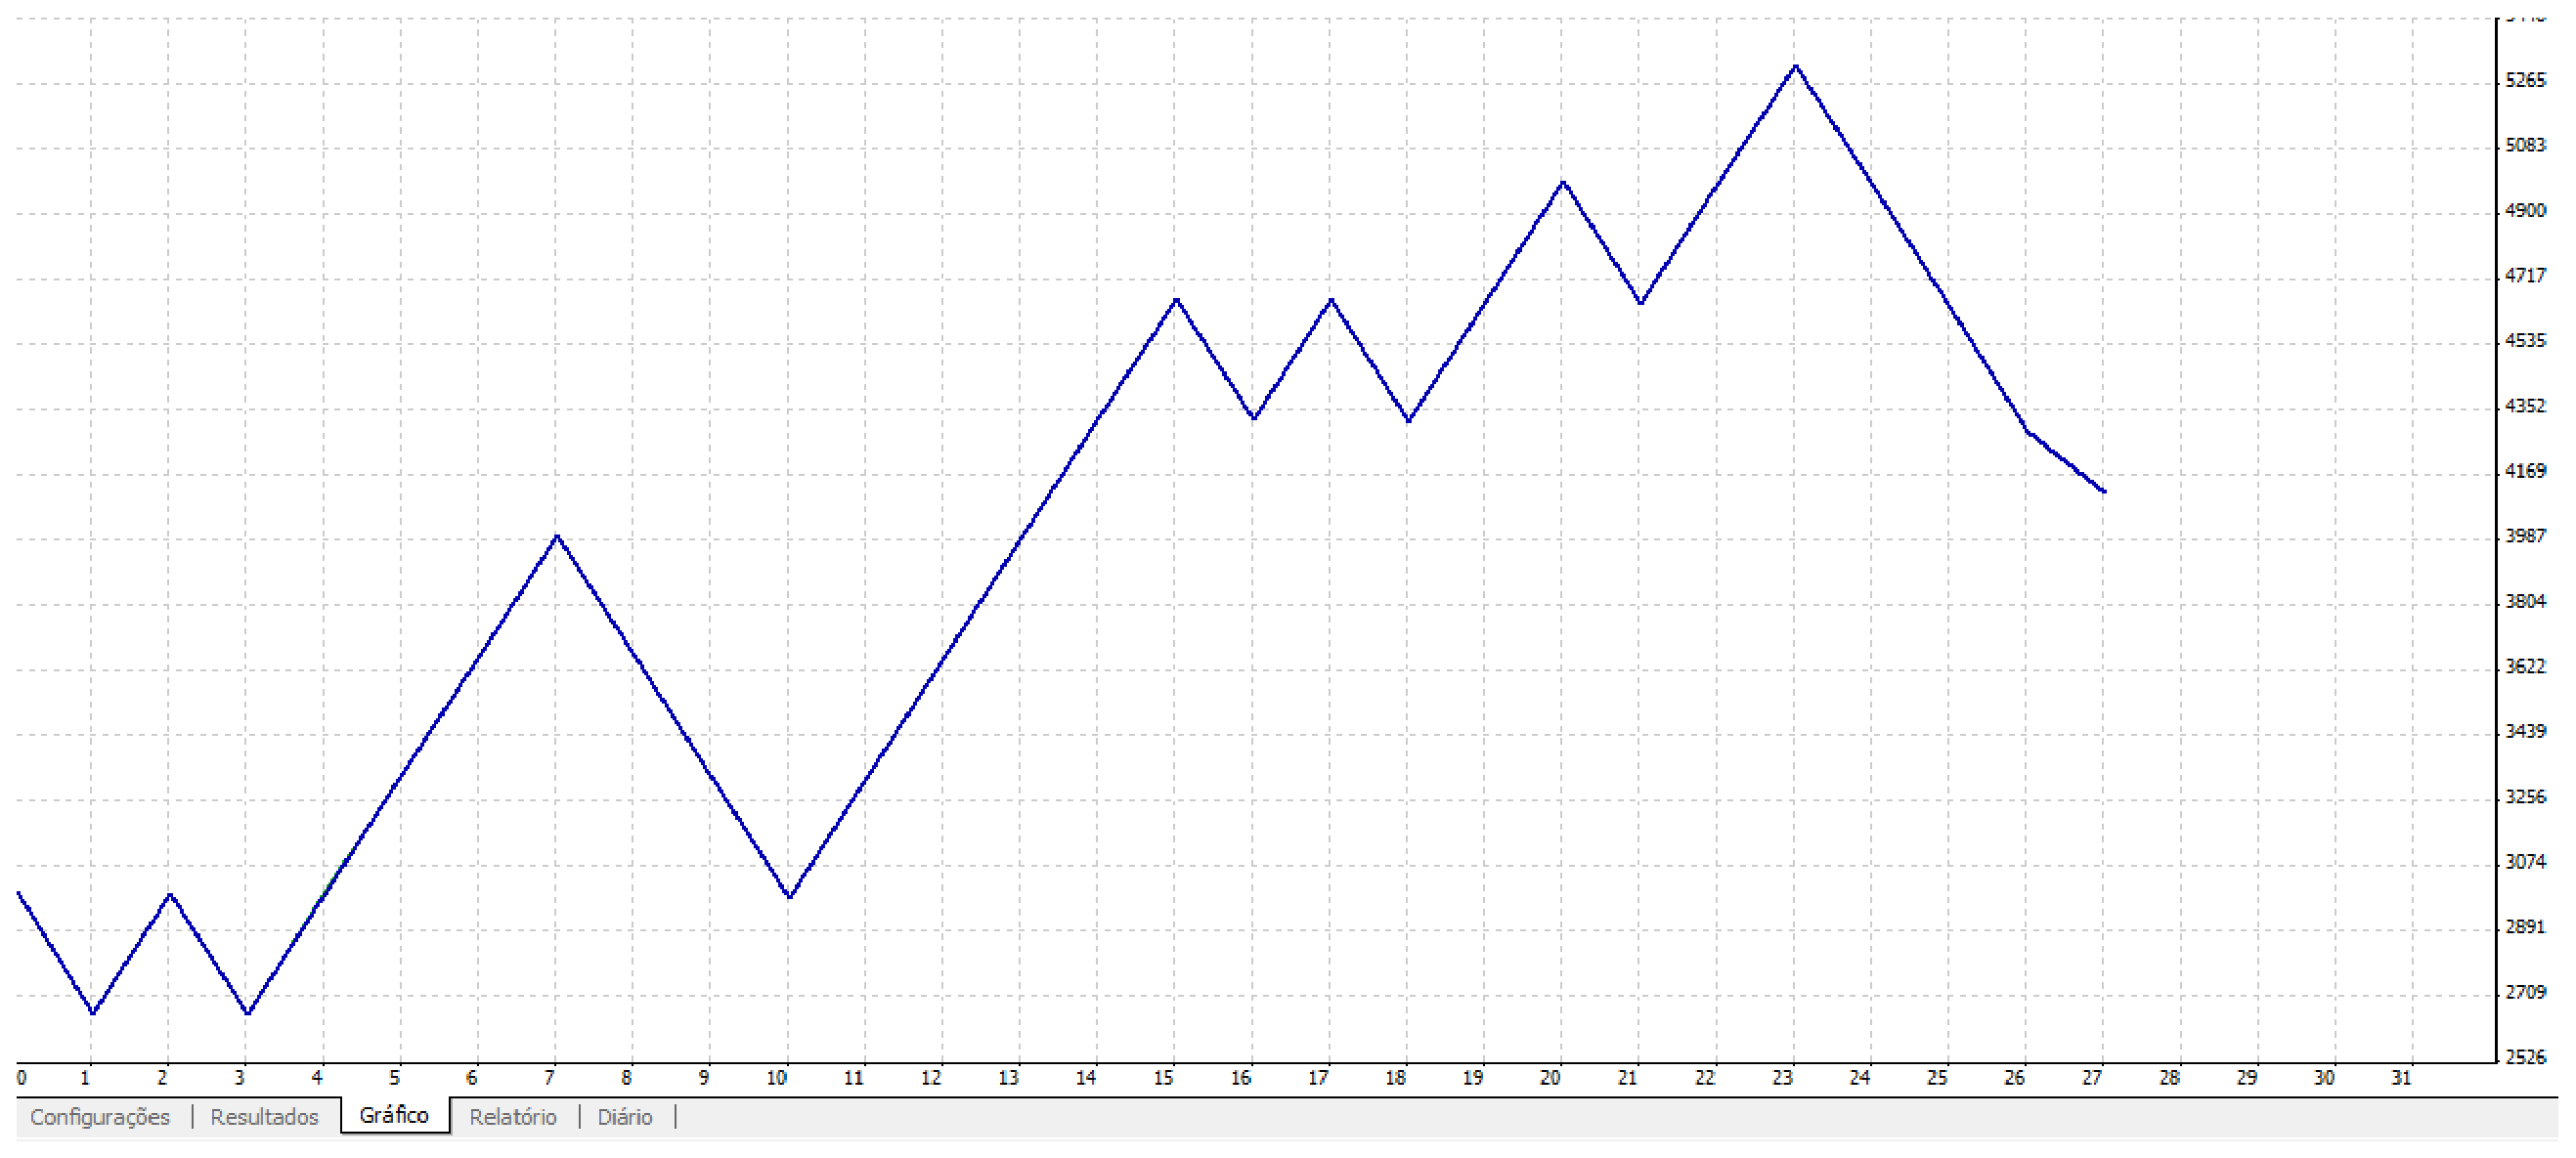
\includegraphics[width=0.9\textwidth]{figuras/protocoloCorrelacao3}
\caption{Gráfico gerado pela simulação do \textit{expert} CorrelacaoPearson.mql no período de Agosto de 2012 a Agosto de 2013}
\label{protocoloCorrelacao3}
\end{figure}

\begin{figure}[H]
\centering
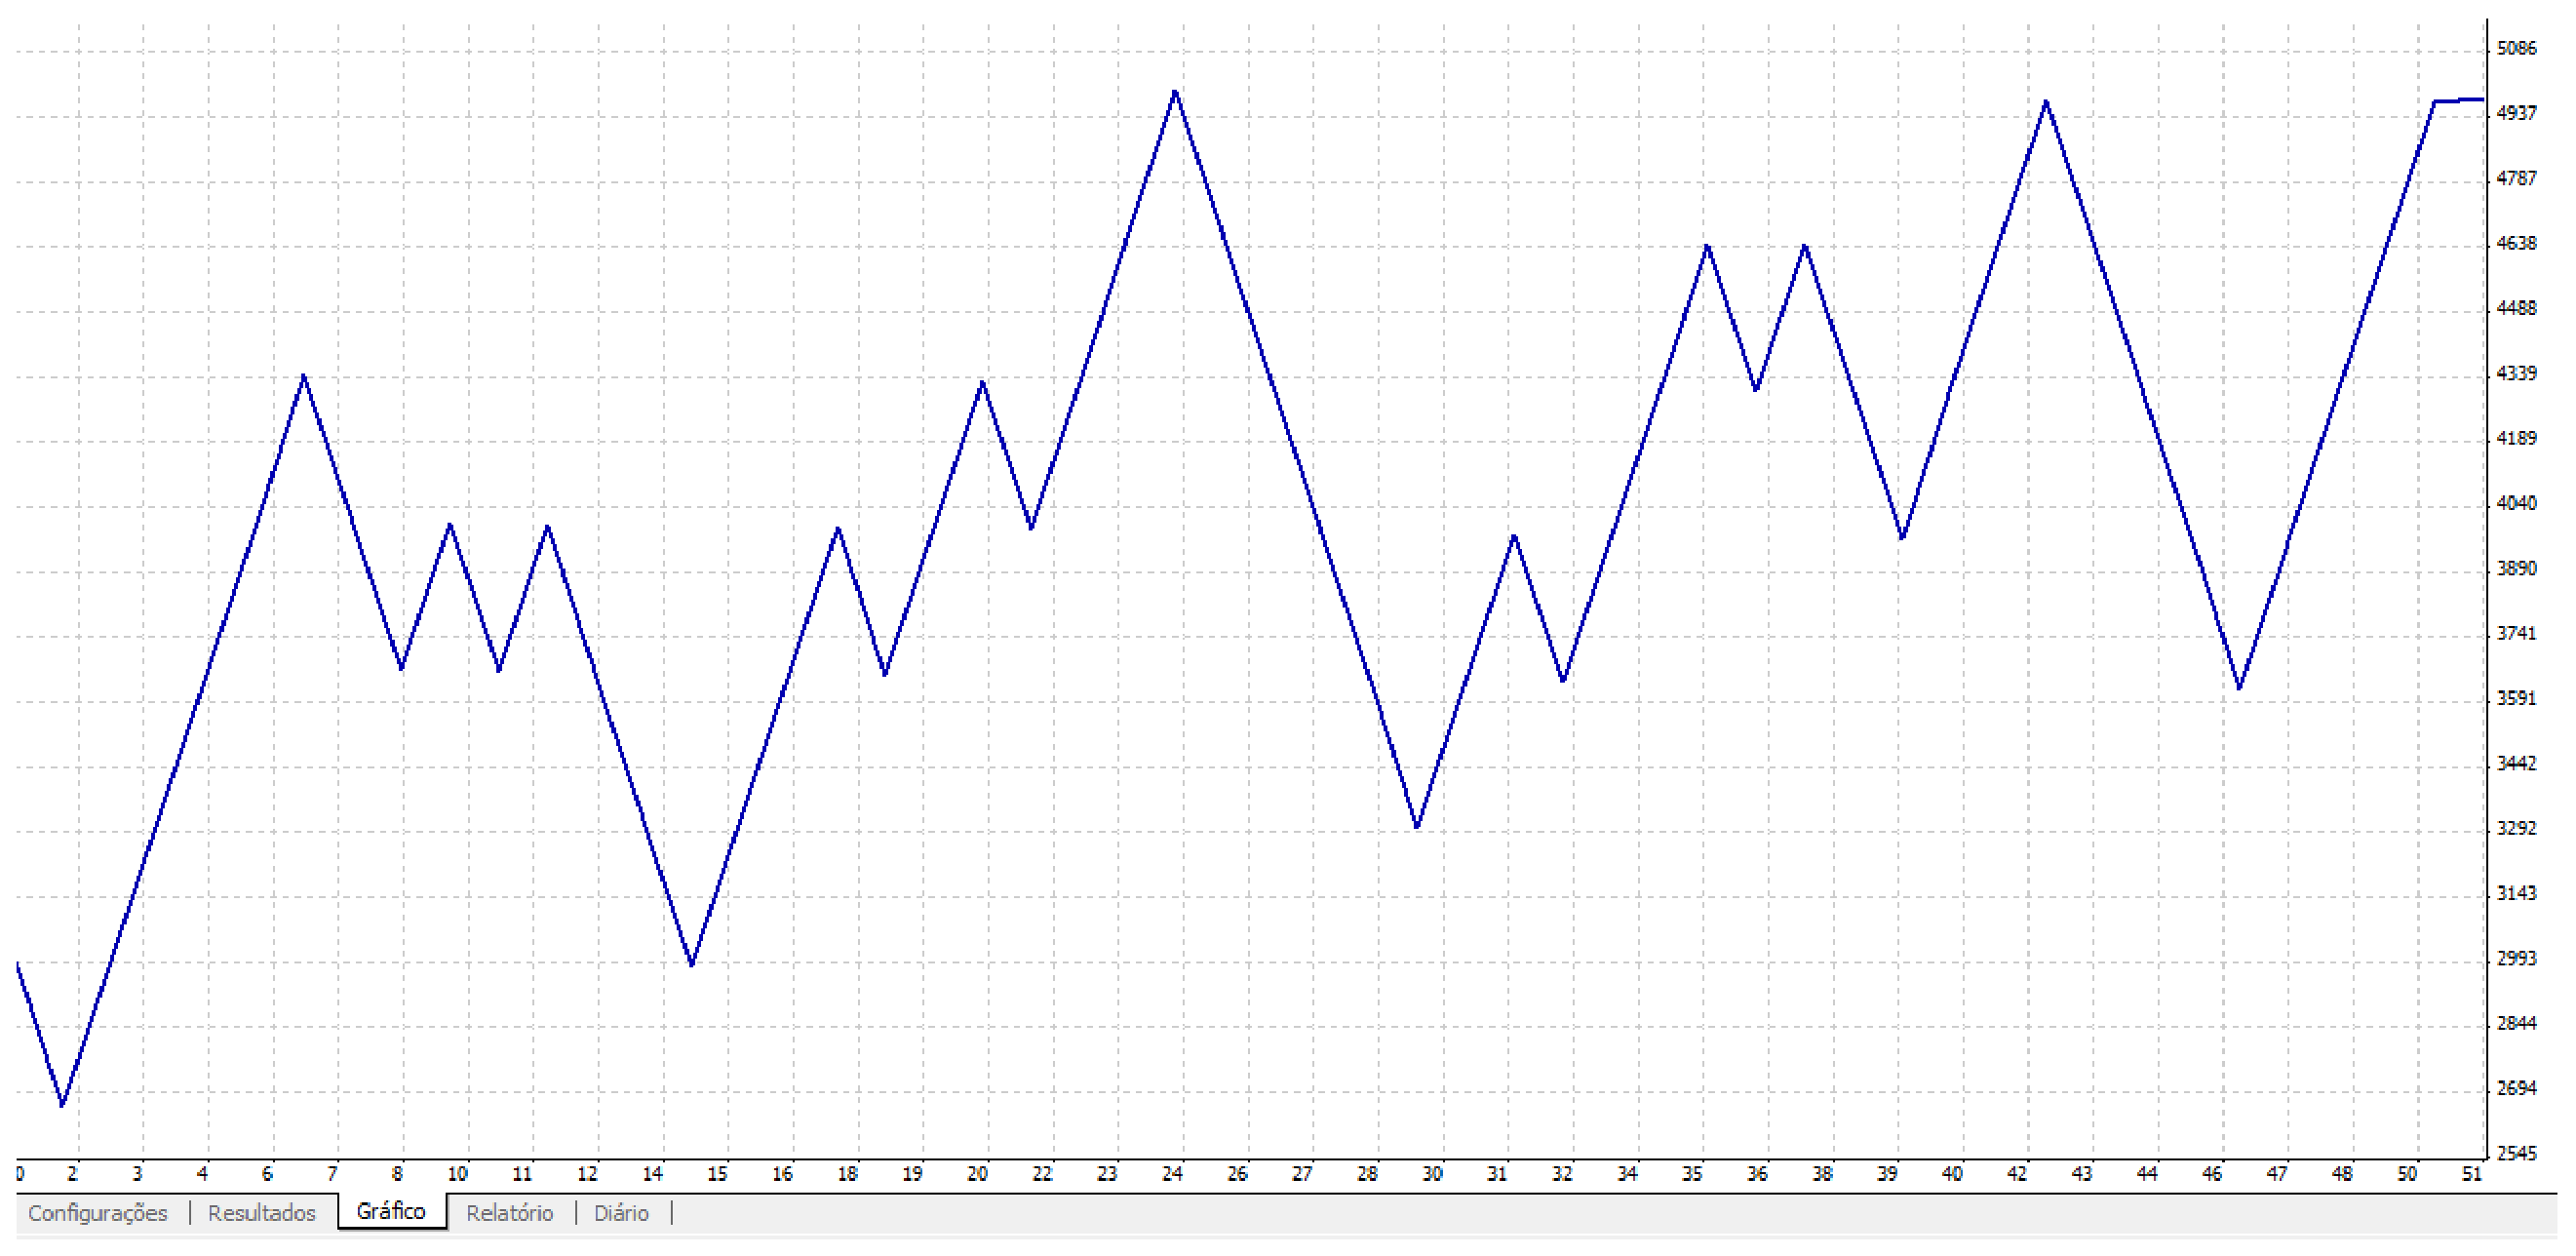
\includegraphics[width=0.9\textwidth]{figuras/protocoloCorrelacao4}
\caption{Gráfico gerado pela simulação do \textit{expert} CorrelacaoPearson.mql no período de Agosto de 2013 a Agosto de 2014}
\label{protocoloCorrelacao4}
\end{figure}

\subsubsection{Simulação do método de Mínimos Quadrados}

O \textit{expert} MinimosQuadrados.mql obteve o percentual de negociações com lucros de 77.88\% no período de Agosto de 2012 a Agosto de 2013 e o  lucro nesse período foi de 1341.88 USD. No período de Agosto de 2013 a Agosto de 2014, o percentual de negociações com lucros foi de 85.71\%  e obteve-se o lucro de 1026 USD. 
Os relatórios completos das simulações podem ser visualizados nas Figuras \ref{protocoloMinimos} e \ref{protocoloMinimos2}.

\begin{figure}[H]
\centering
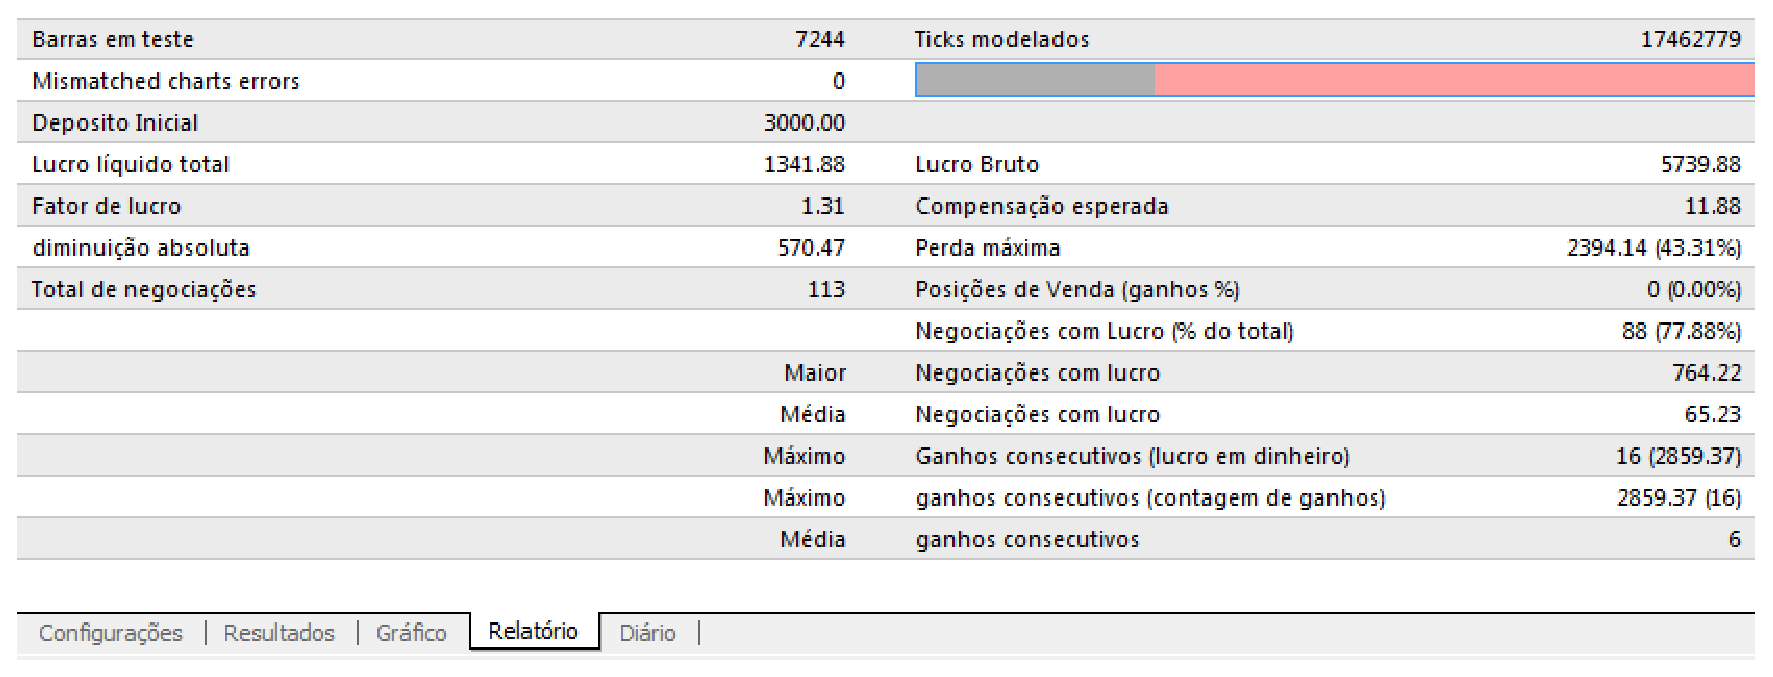
\includegraphics[width=0.9\textwidth]{figuras/protocoloMinimos}
\caption{Relatório de simulação no período de Agosto de 2012 a Agosto de 2013 do \textit{expert}}
\label{protocoloMinimos}
\end{figure}

\begin{figure}[H]
\centering
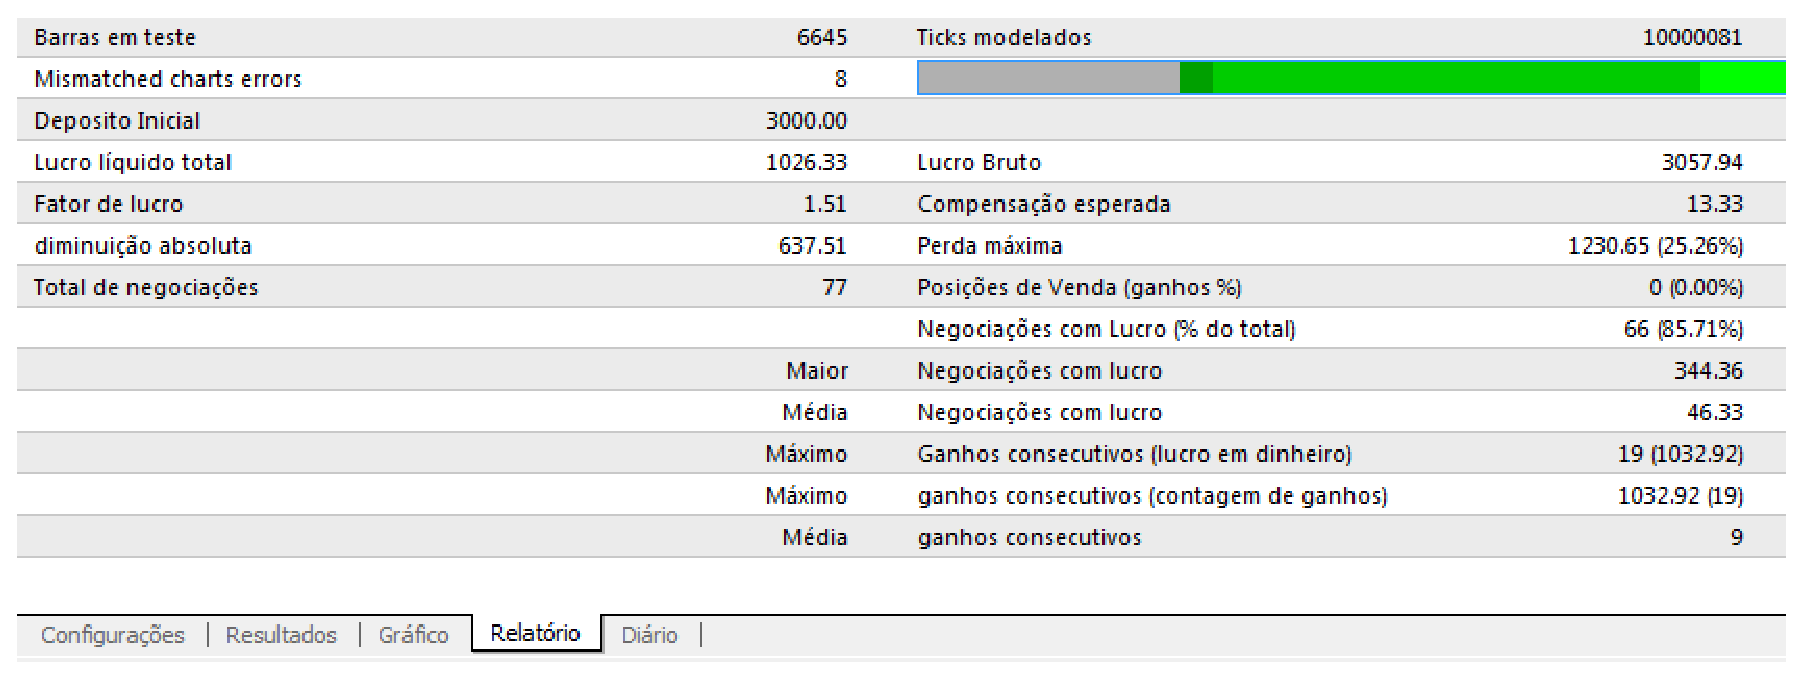
\includegraphics[width=0.9\textwidth]{figuras/protocoloMinimos2}
\caption{Relatório de simulação no período de Agosto de 2012 a Agosto de 2013 do \textit{expert}}
\label{protocoloMinimos2}
\end{figure}

O \textit{expert} MinimosQuadrados.mql, teve altos e baixos nas simulações durante os dois anos (2012 a 2013 e 2013 a 2014). Mas, no desempenho geral, conforme é evidenciado nos gráficos, o \textit{expert} teve um desempenho satisfatório.

\begin{figure}[H]
\centering
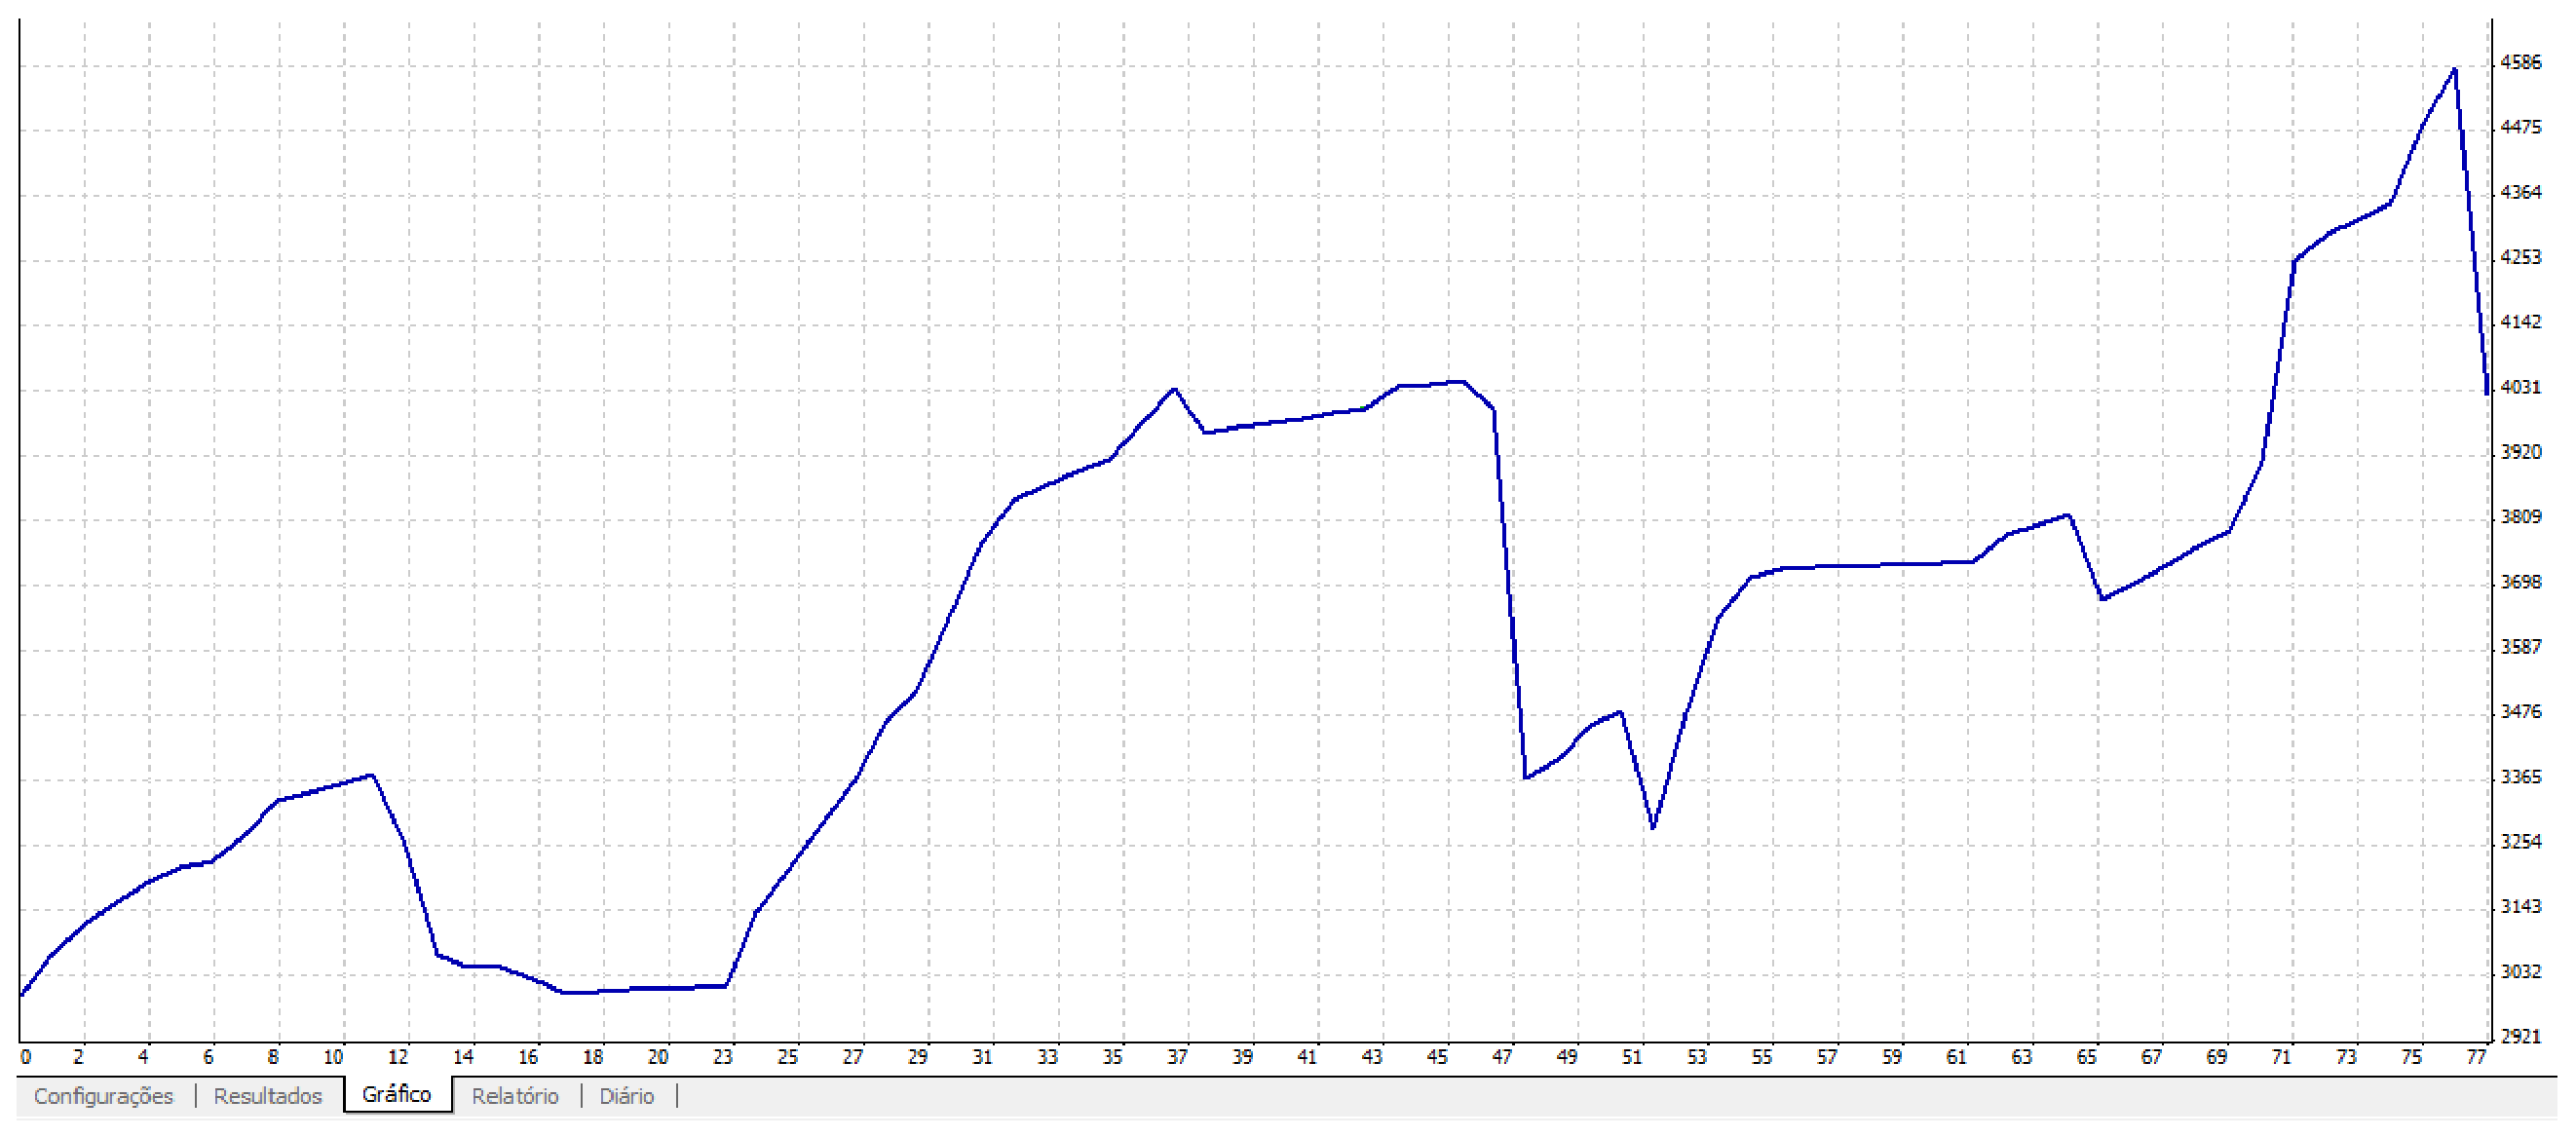
\includegraphics[width=0.9\textwidth]{figuras/protocoloMinimos3}
\caption{Relatório de simulação no período de Agosto de 2012 a Agosto de 2013 do \textit{expert}}
\label{protocoloMinimos3}
\end{figure}

\begin{figure}[H]
\centering
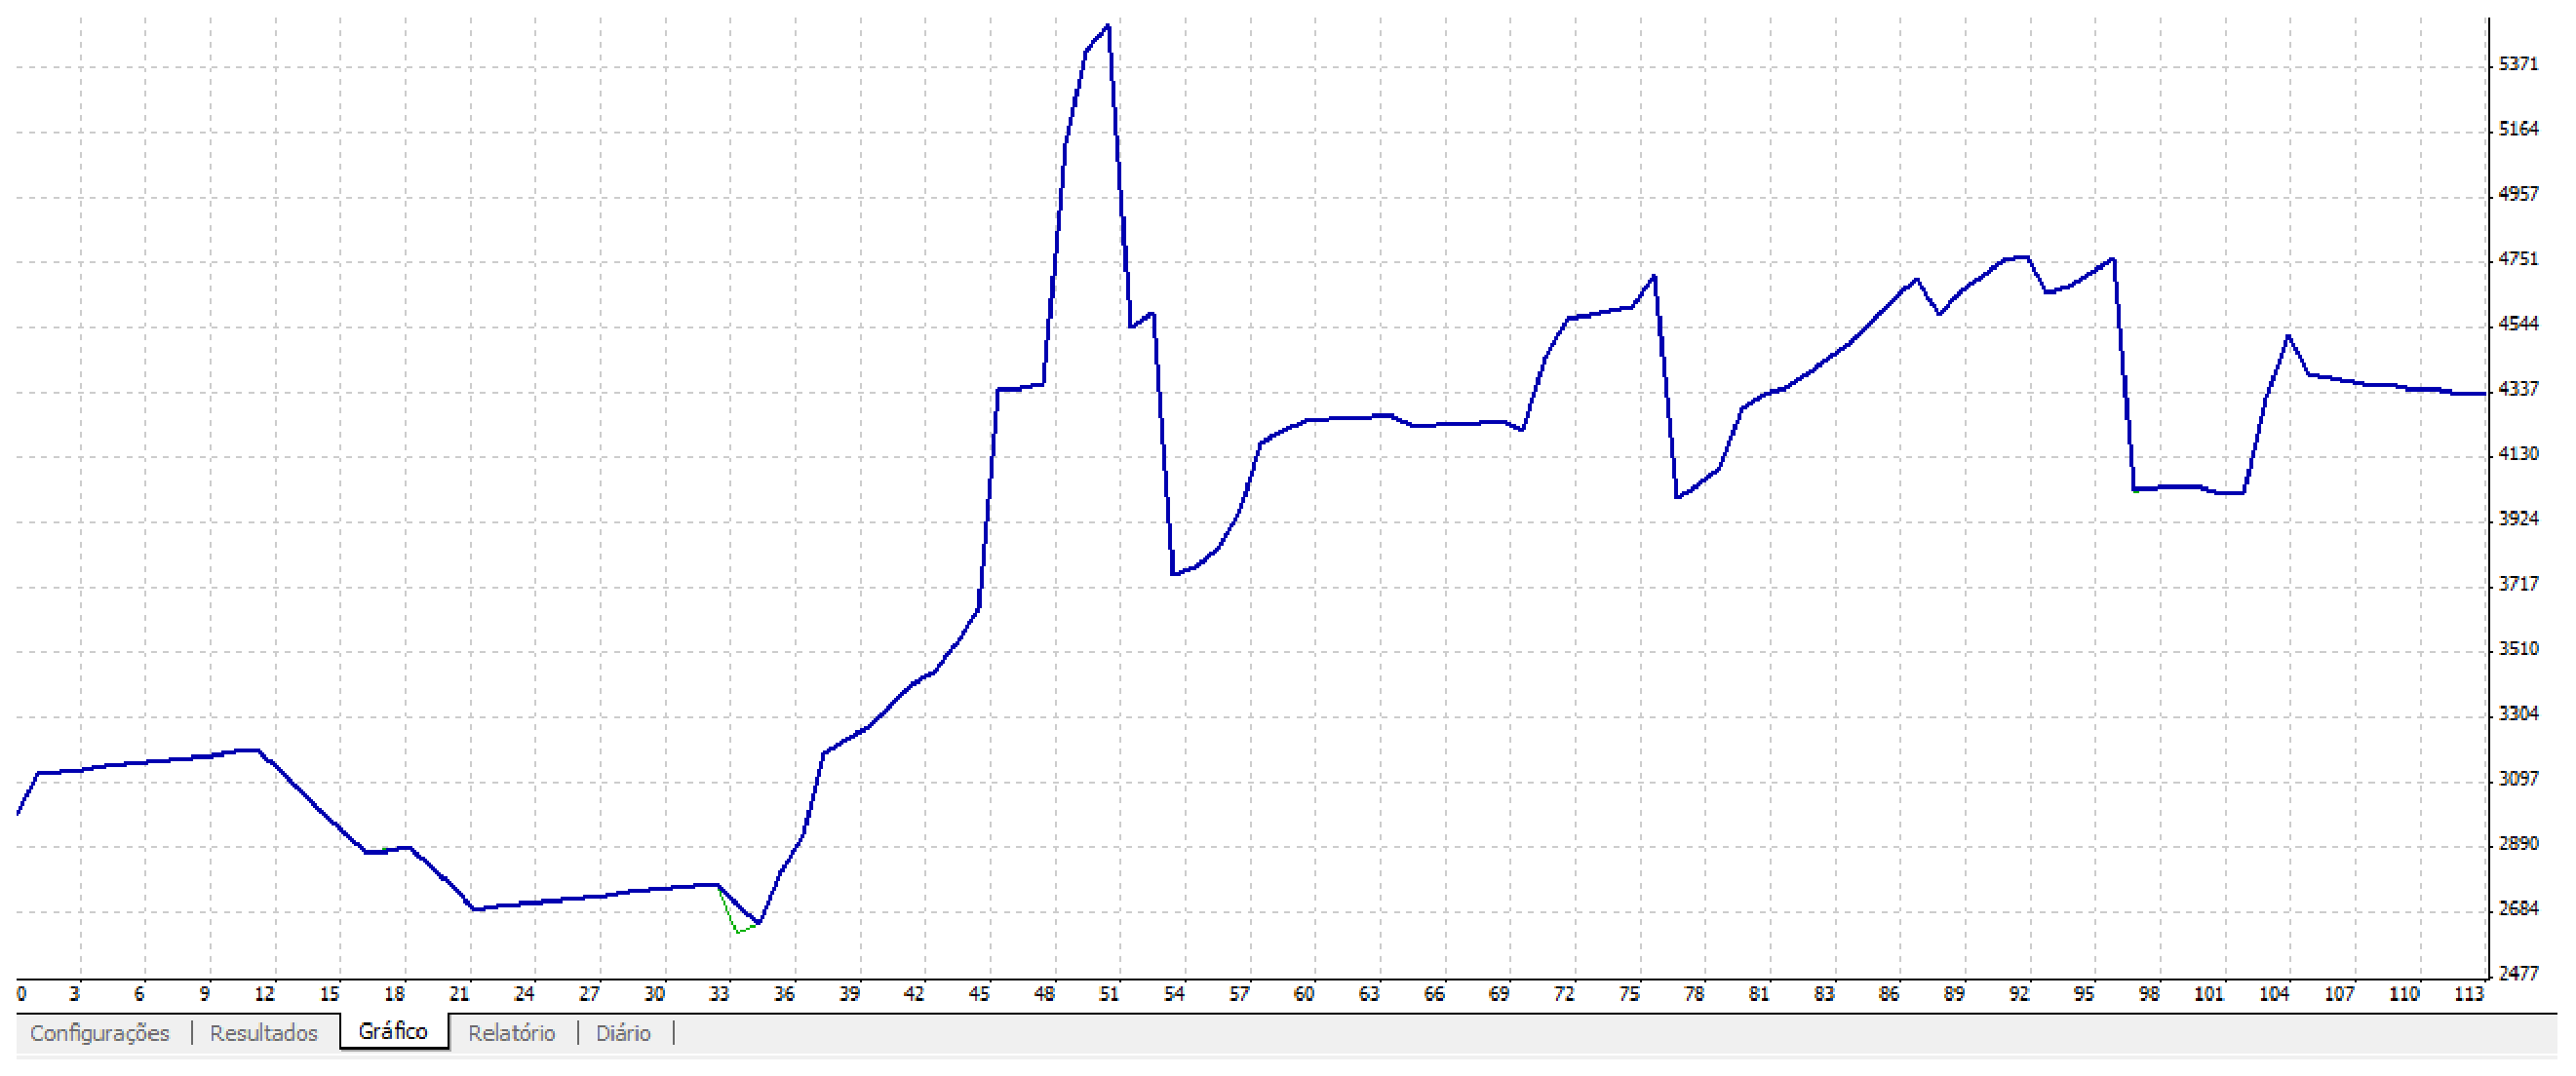
\includegraphics[width=0.9\textwidth]{figuras/protocoloMinimos4}
\caption{Relatório de simulação no período de Agosto de 2013 a Agosto de 2014 do \textit{expert}}
\label{protocoloMinimos4}
\end{figure}

\subsubsection{Simulação do método de Fibonacci}

O \textit{expert} Fibonacci.mql obteve o percentual de negociações com lucros de 72.73\% no período de Agosto de 2012 a Agosto de 2013 e o  lucro nesse período foi de 341.20 USD.
No período de Agosto de 2013 a Agosto de 2014, o percentual de negociações com lucros foi de 56.00\%  e obteve-se o lucro de 659.05 USD. Apesar do percentual de acerto nesse período ter sido menor quando comparado ao período de agosto 2012-2013, o lucro obtido foi 51.77\% maior. Isso se deve ao fato de no período de agosto 2013-2014, o \textit{expert} ter negociado mais vezes (25 contra 11).

Os relatórios completos das simulações podem ser visualizados nas Figuras \ref{protocoloFib} e \ref{protocoloFib2}.

\begin{figure}[H]
\centering
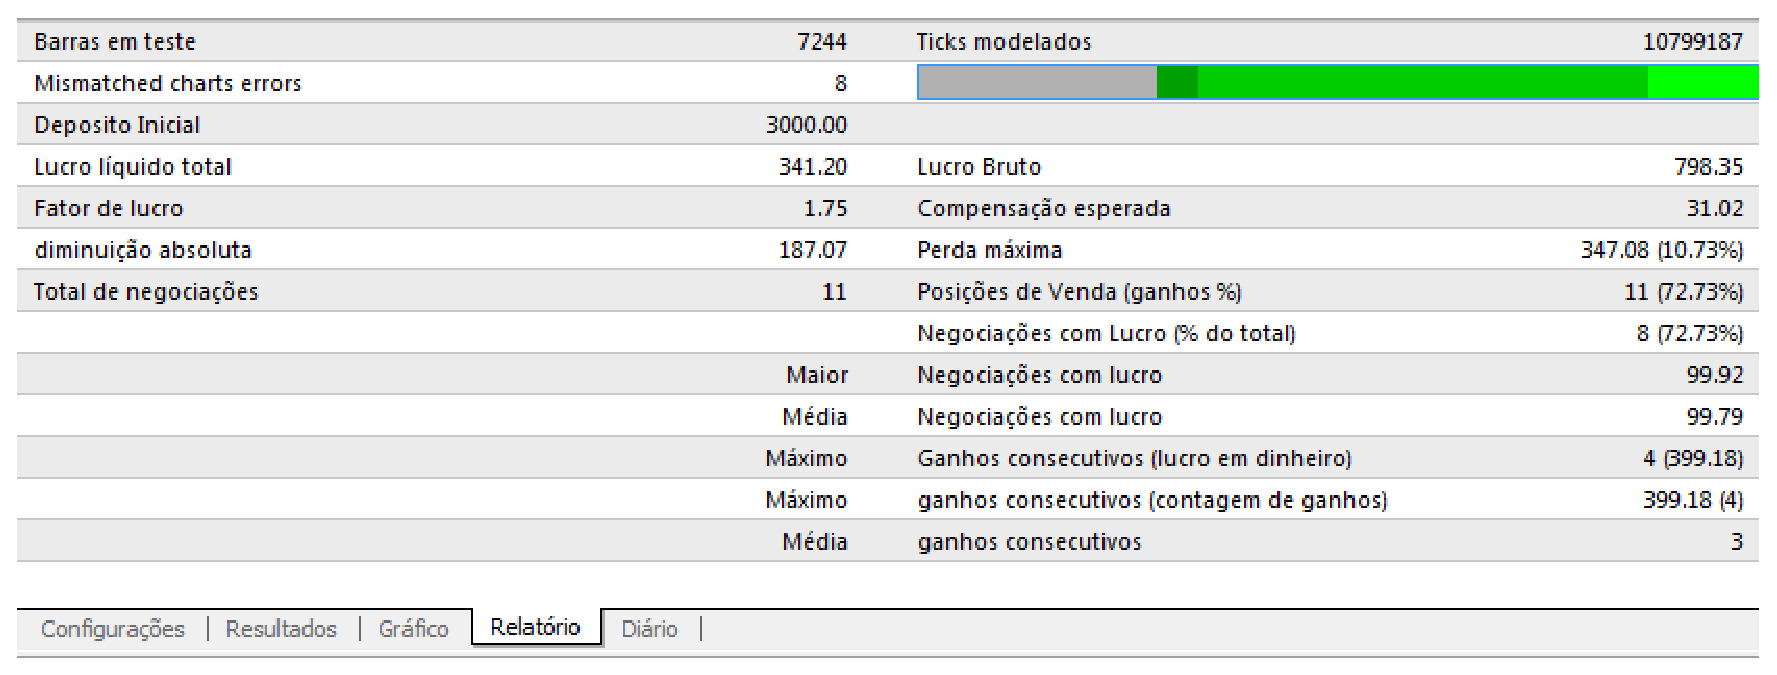
\includegraphics[width=0.9\textwidth]{figuras/protocoloFib}
\caption{Relatório de simulação no período de Agosto de 2012 s Agosto de 2013 do \textit{expert}}
\label{protocoloFib}
\end{figure}

\begin{figure}[H]
\centering
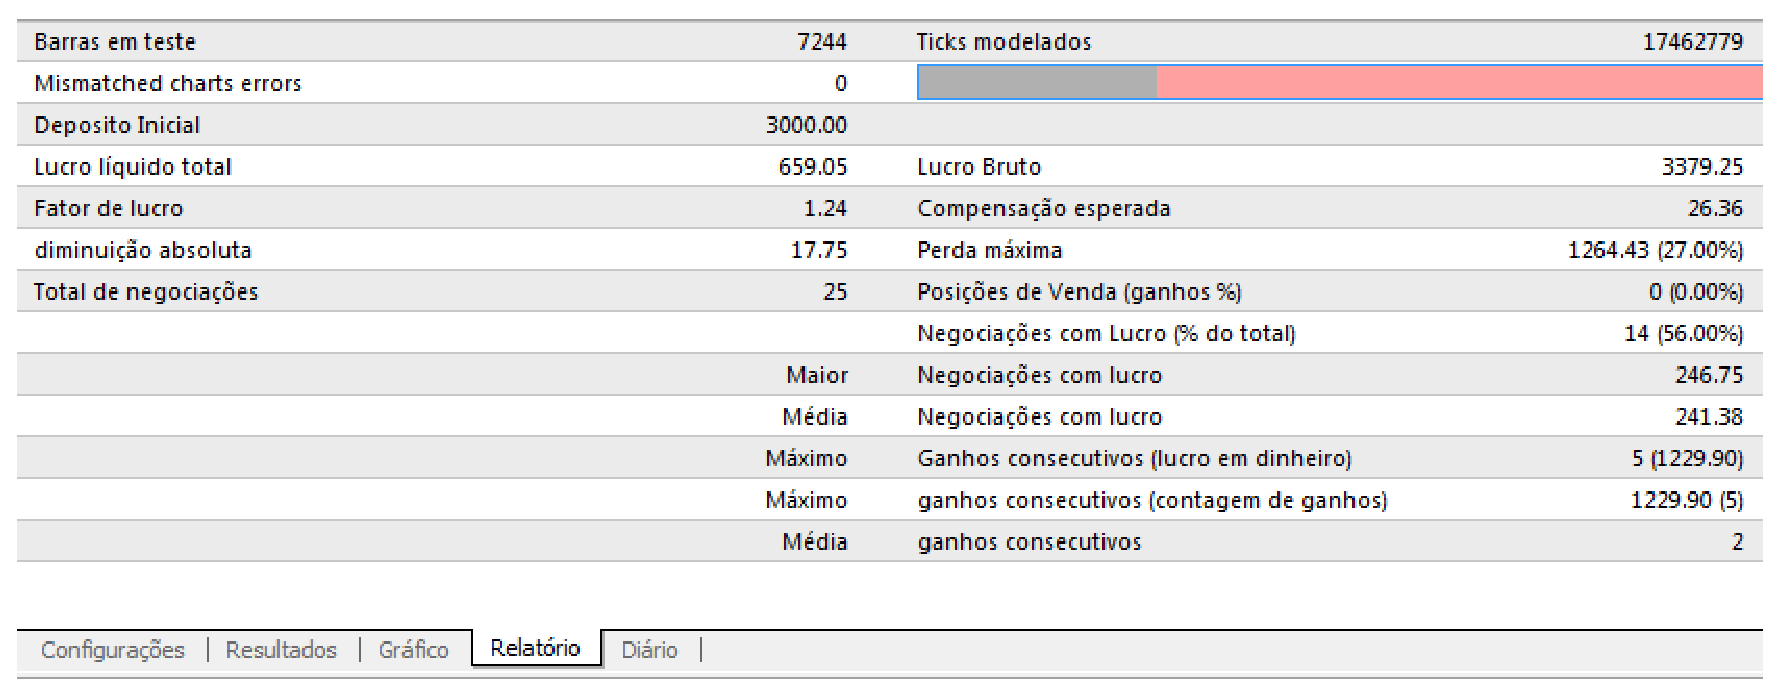
\includegraphics[width=0.9\textwidth]{figuras/protocoloFib2}
\caption{Relatório de simulação no período agosto 2013-2014 do \textit{expert}}
\label{protocoloFib2}
\end{figure}

É possível visualizar nos gráficos das simulações, os lucros de capital que o \textit{expert} Fibonacci.mql gerou.

\begin{figure}[H]
\centering
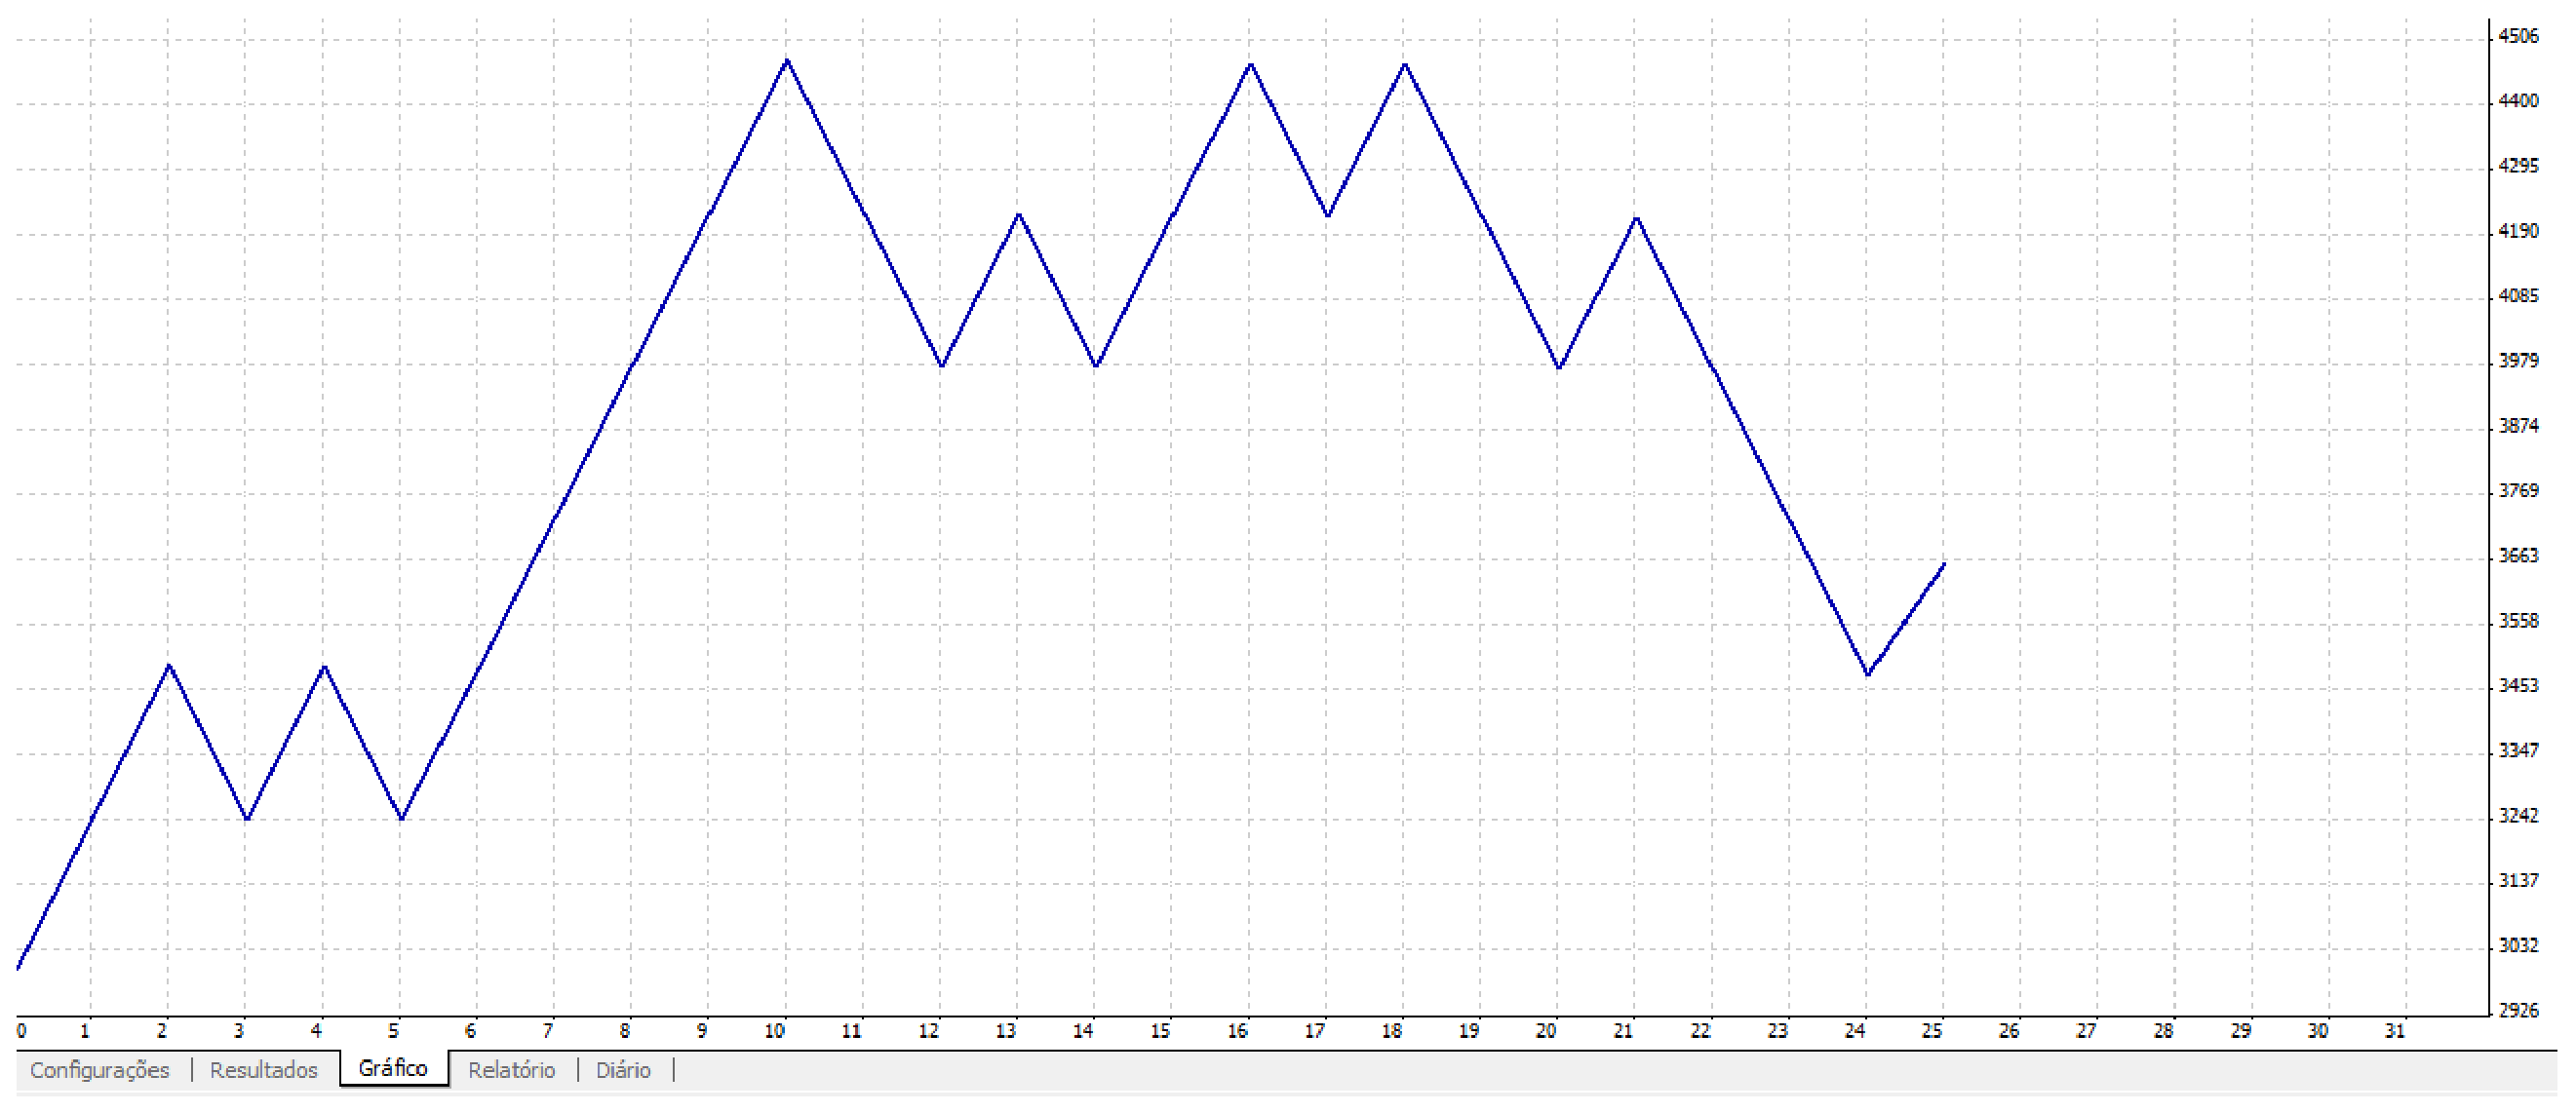
\includegraphics[width=0.9\textwidth]{figuras/protocoloFib3}
\caption{Gráfico gerado pela simulação do \textit{expert} Fibonacci.mql no período de Agosto de 2012 a Agosto de 2013}
\label{protocoloFib3}
\end{figure}

\begin{figure}[H]
\centering
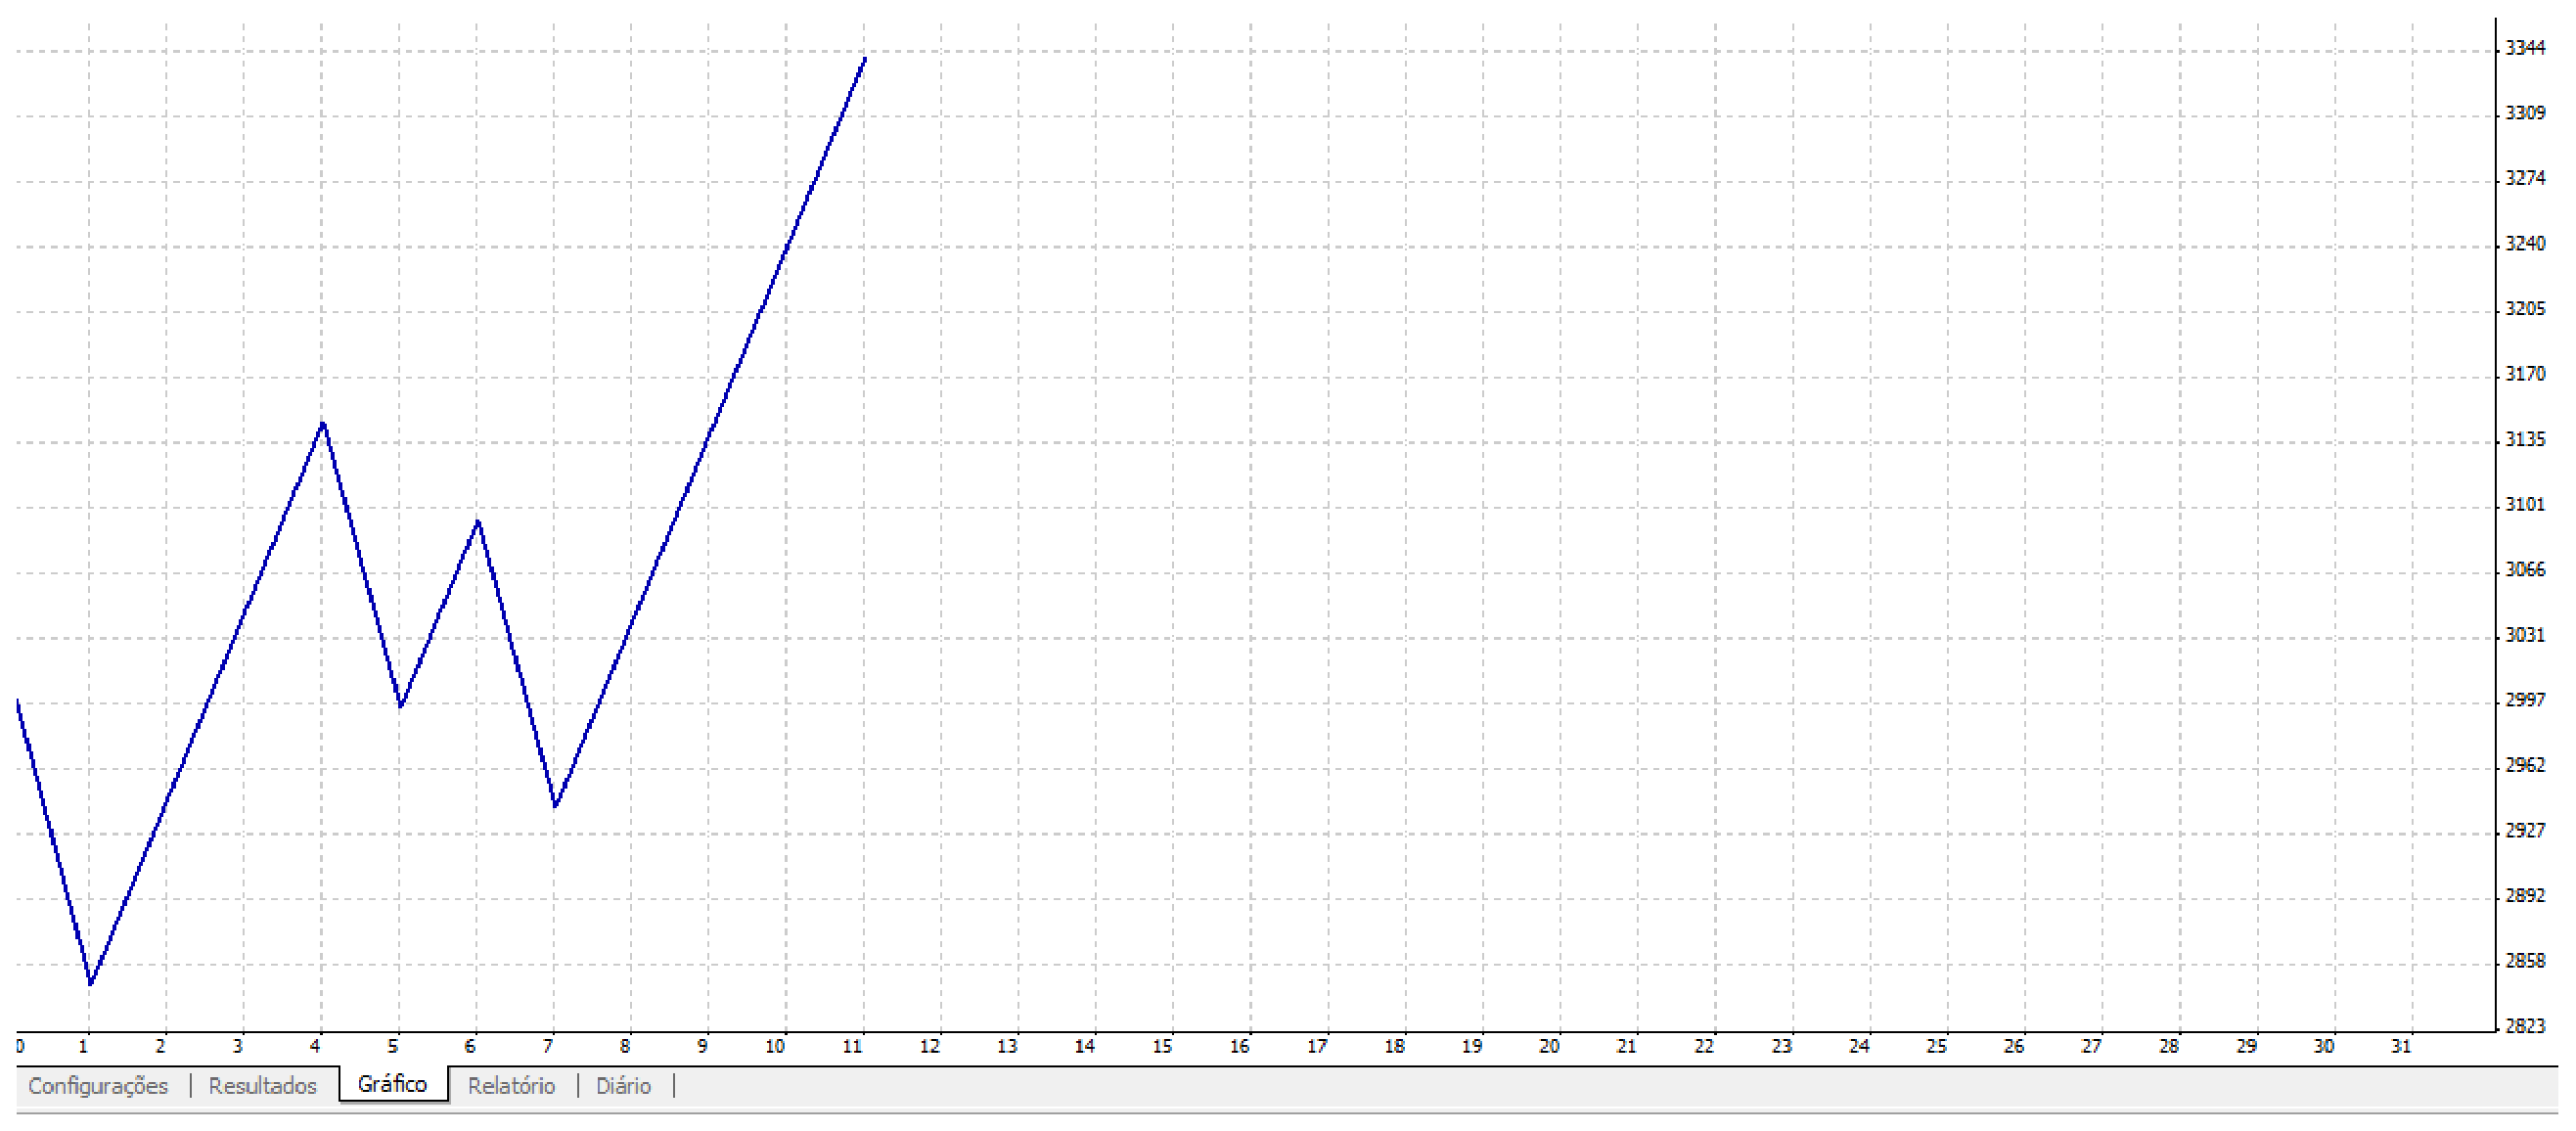
\includegraphics[width=0.9\textwidth]{figuras/protocoloFib4}
\caption{Gráfico gerado pela simulação do \textit{expert} Fibonacci.mql no período de Agosto de 2013 a Agosto de 2014}
\label{protocoloFib4}
\end{figure}

\subsubsection{Simulação do método de Estocástico}

O \textit{expert} Estocastico.mql obteve o percentual de negociações com lucros de 47.47\% no período agosto 2012-2013. Portanto, o percentual de negociações com perdas foi de 52.53\%. Nesse período, o \textit{expert} teve um prejuízo de 1110.88 USD.

No período de Agosto de 2013 a Agosto de 2014, o percentual de negociações com lucros foi de 47.70\% (percentual com perdas de 52.30\%)  e obteve-se o prejuízo de 459.17 USD. 
Os relatórios completos das simulações podem ser visualizados nas Figuras \ref{protocoloEst} e \ref{protocoloEst2}.

\begin{figure}[H]
\centering
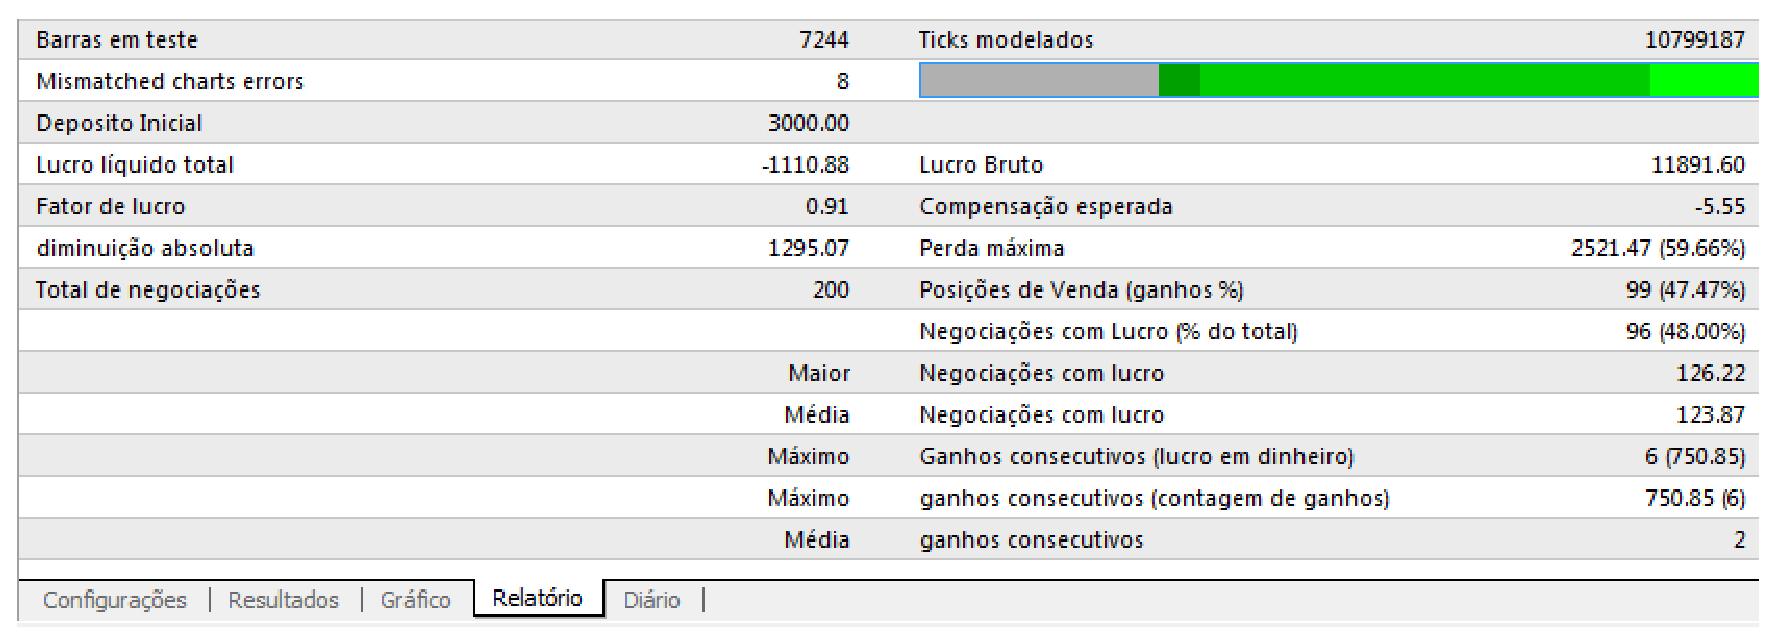
\includegraphics[width=0.9\textwidth]{figuras/protocoloEst}
\caption{Relatório de simulação no período de Agosto de 2012 a Agosto de 2013 do \textit{expert} Estocastico.mql}
\label{protocoloEst}
\end{figure}

\begin{figure}[H]
\centering
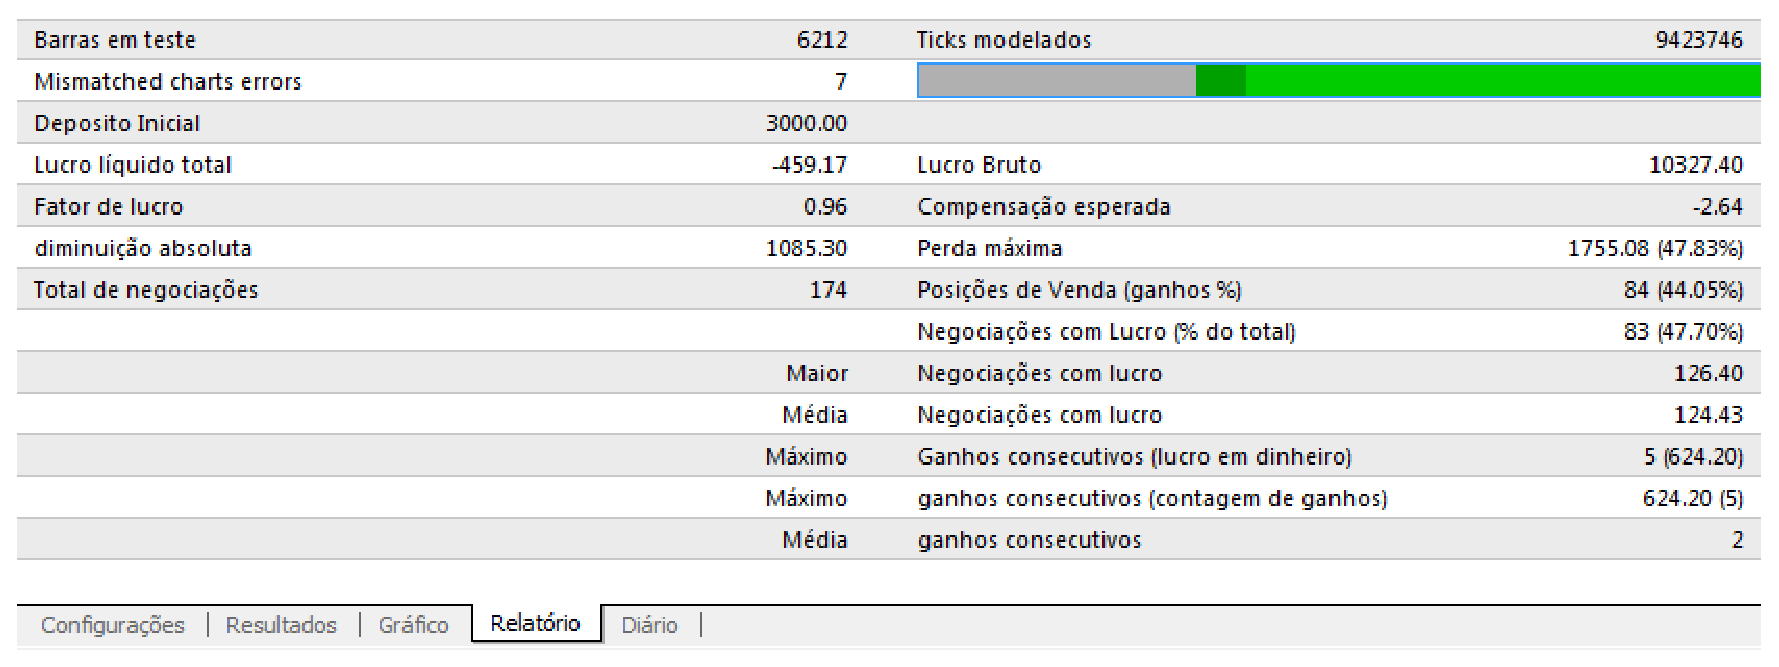
\includegraphics[width=0.9\textwidth]{figuras/protocoloEst2}
\caption{Relatório de simulação no período de Agosto de 2013 a Agosto de 2014 do \textit{expert} Estocastico.mql}
\label{protocoloEst2}
\end{figure}

É possível visualizar nos gráficos das simulações, as perdas de capital que o \textit{expert} Estocastico.mql gerou.

\begin{figure}[H]
\centering
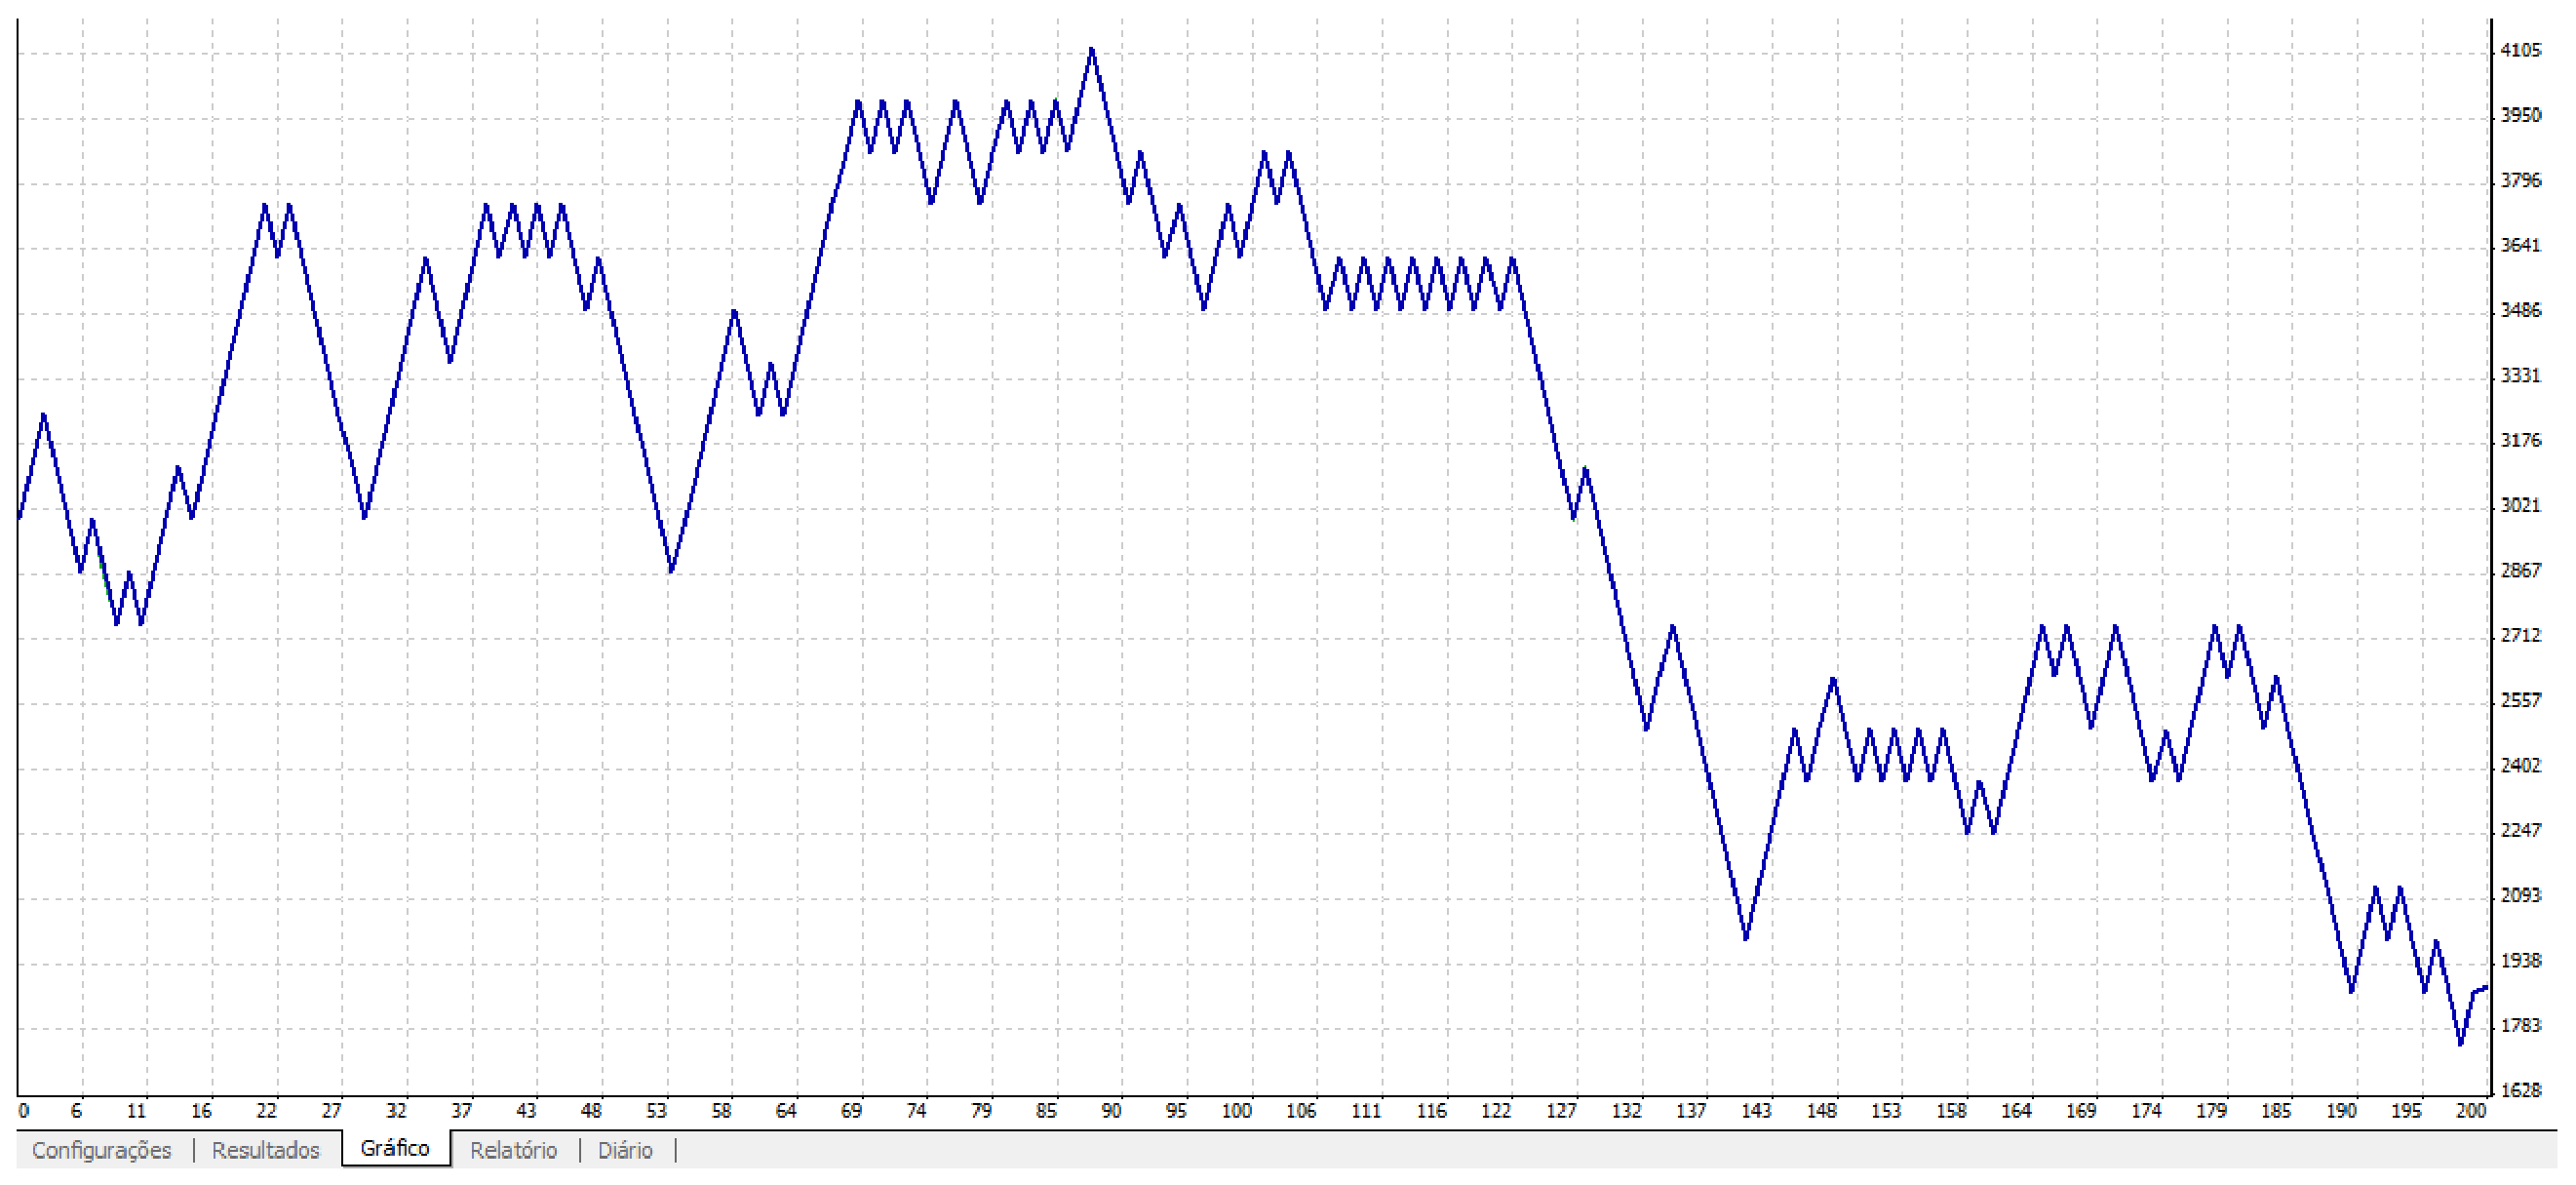
\includegraphics[width=0.9\textwidth]{figuras/protocoloEst3}
\caption{Gráfico gerado pela simulação do \textit{expert} Estocastico.mql no período de Agosto de 2012 a Agosto de 2013} 
\label{protocoloEst3}
\end{figure}

\begin{figure}[H]
\centering
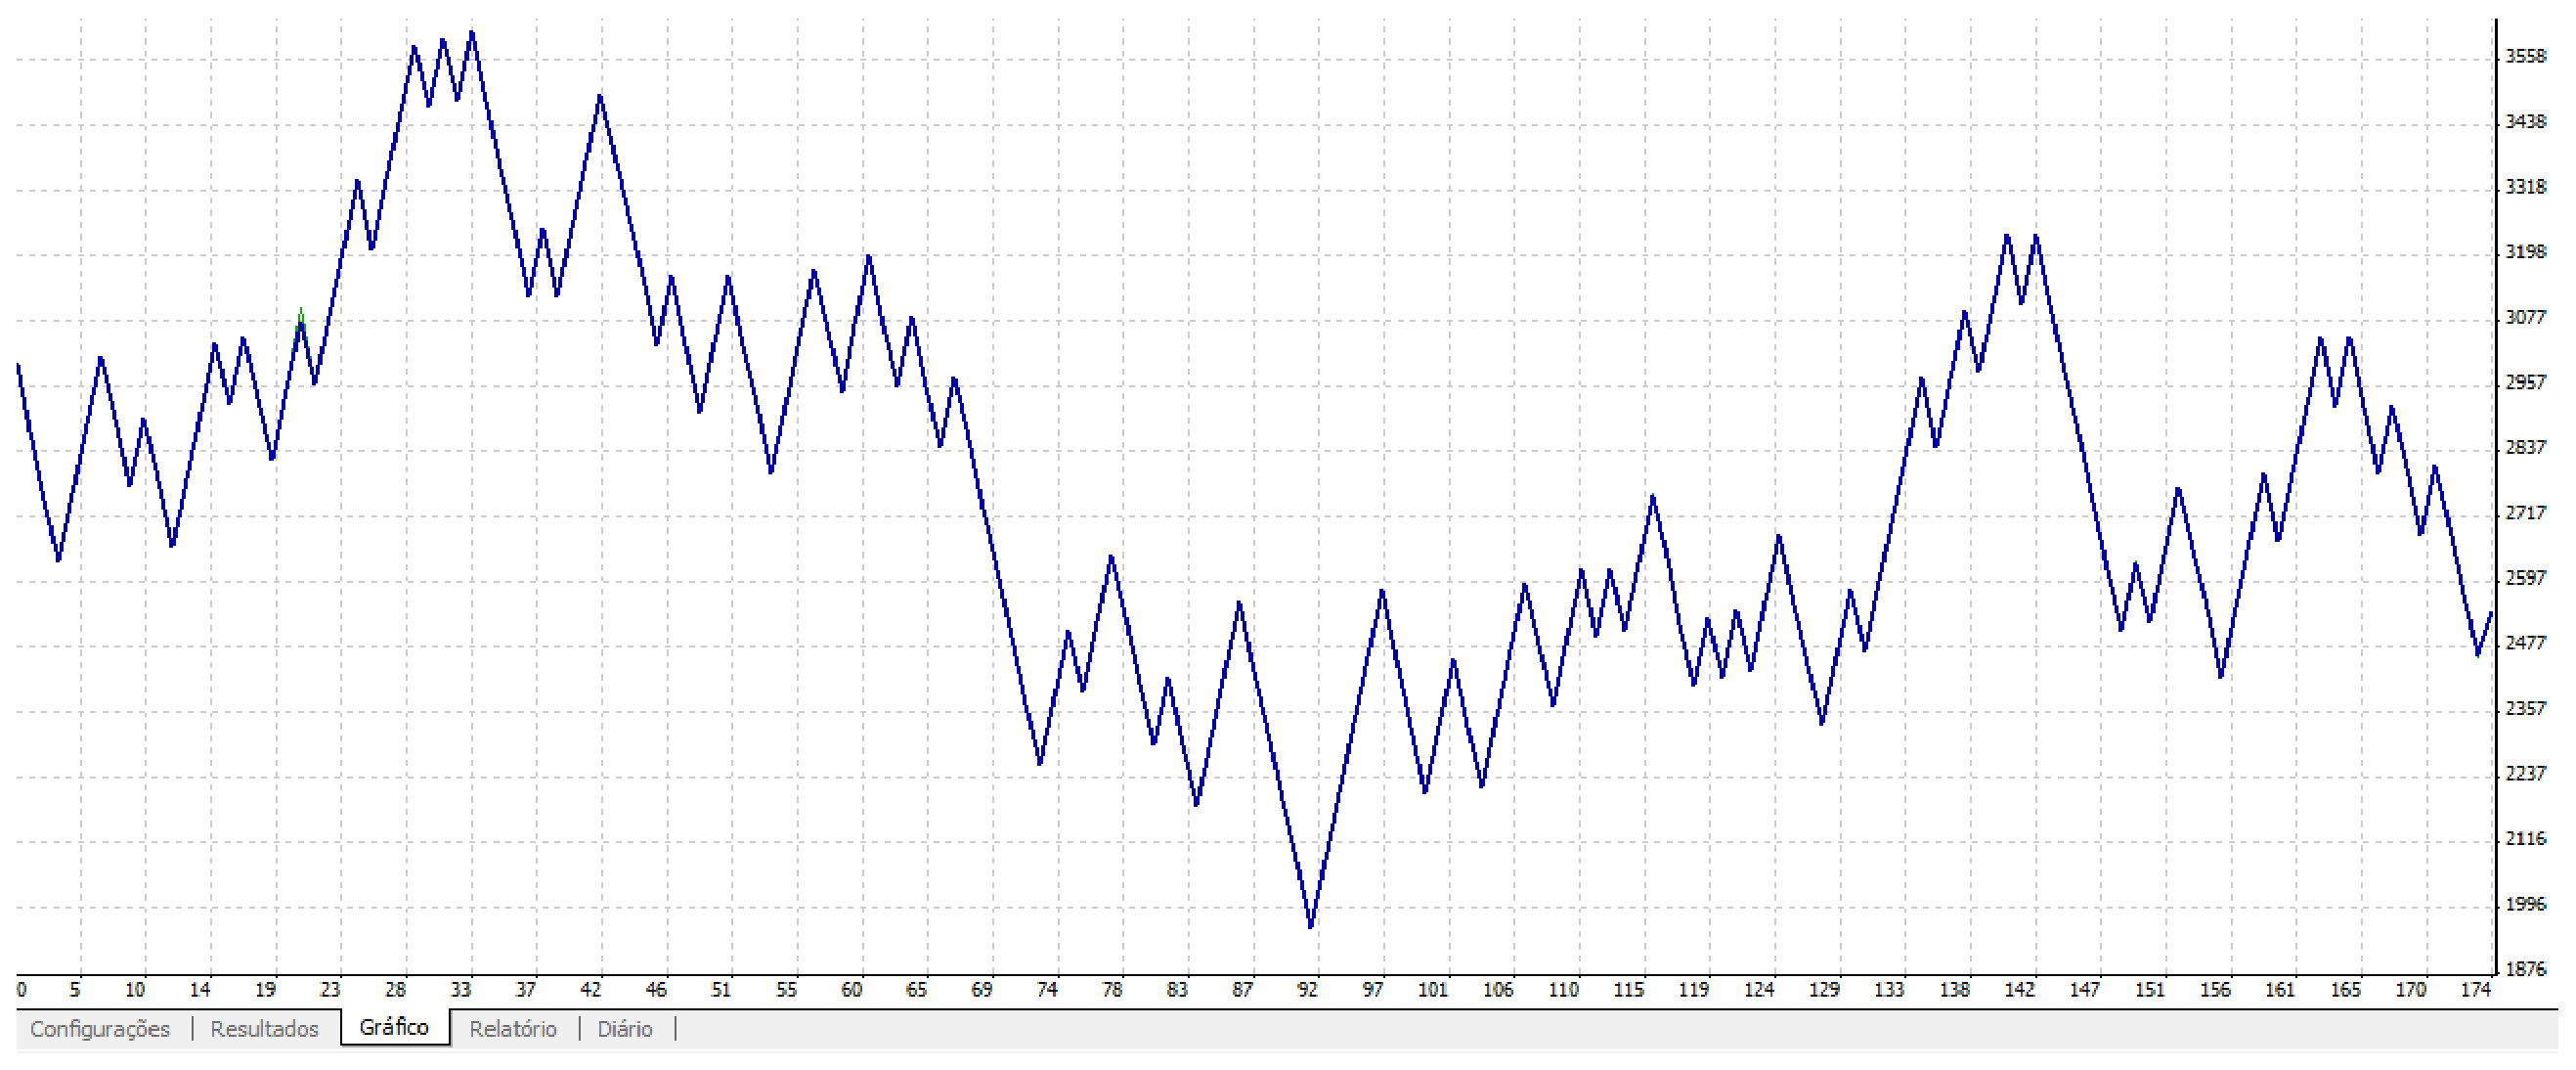
\includegraphics[width=0.9\textwidth]{figuras/protocoloEst4}
\caption{Gráfico gerado pela simulação do \textit{expert} Estocastico.mql no período de Agosto de 2013 a Agosto de 2014} 
\label{protocoloEst4}
\end{figure}

\subsubsection{Simulação do método de Média Móvel}

O \textit{expert} MediaMovel.mql obteve o percentual de negociações com lucros de 43.55\% no período de Agosto de 2012 a Agosto de 2013. Portanto, o percentual de negociações com perdas foi de 56.45\%. Nesse período, o \textit{expert} obteve um prejuízo de 2987.00 USD. 

No período de Agosto de 2013 a Agosto de  2014, o percentual de negociações com lucros foi de 48.48\% e o percentual de negociação com prejuízos foi de 51.82\%.  Foi obtido o prejuízo de 459.17 USD. 

Os relatórios completos das simulações podem ser visualizados nas Figuras \ref{protocoloMedia} e \ref{protocoloMedia2}.

\begin{figure}[H]
\centering
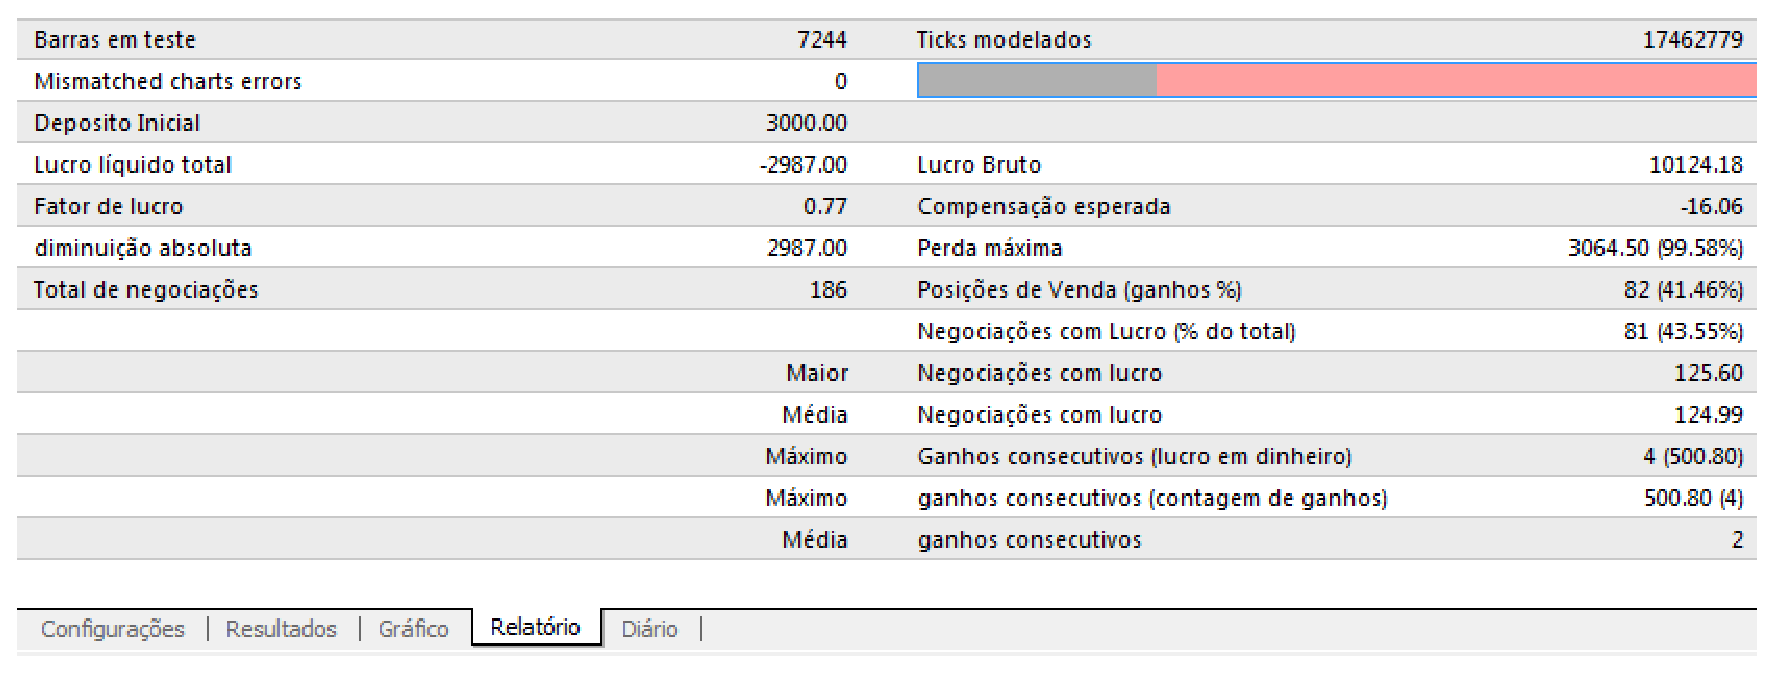
\includegraphics[width=0.9\textwidth]{figuras/protocoloMedia}
\caption{Relatório de simulação no período de Agosto de 2012 a Agosto de 2013 do \textit{expert} MediaMovel.mql} 
\label{protocoloMedia}
\end{figure}

\begin{figure}[H]
\centering
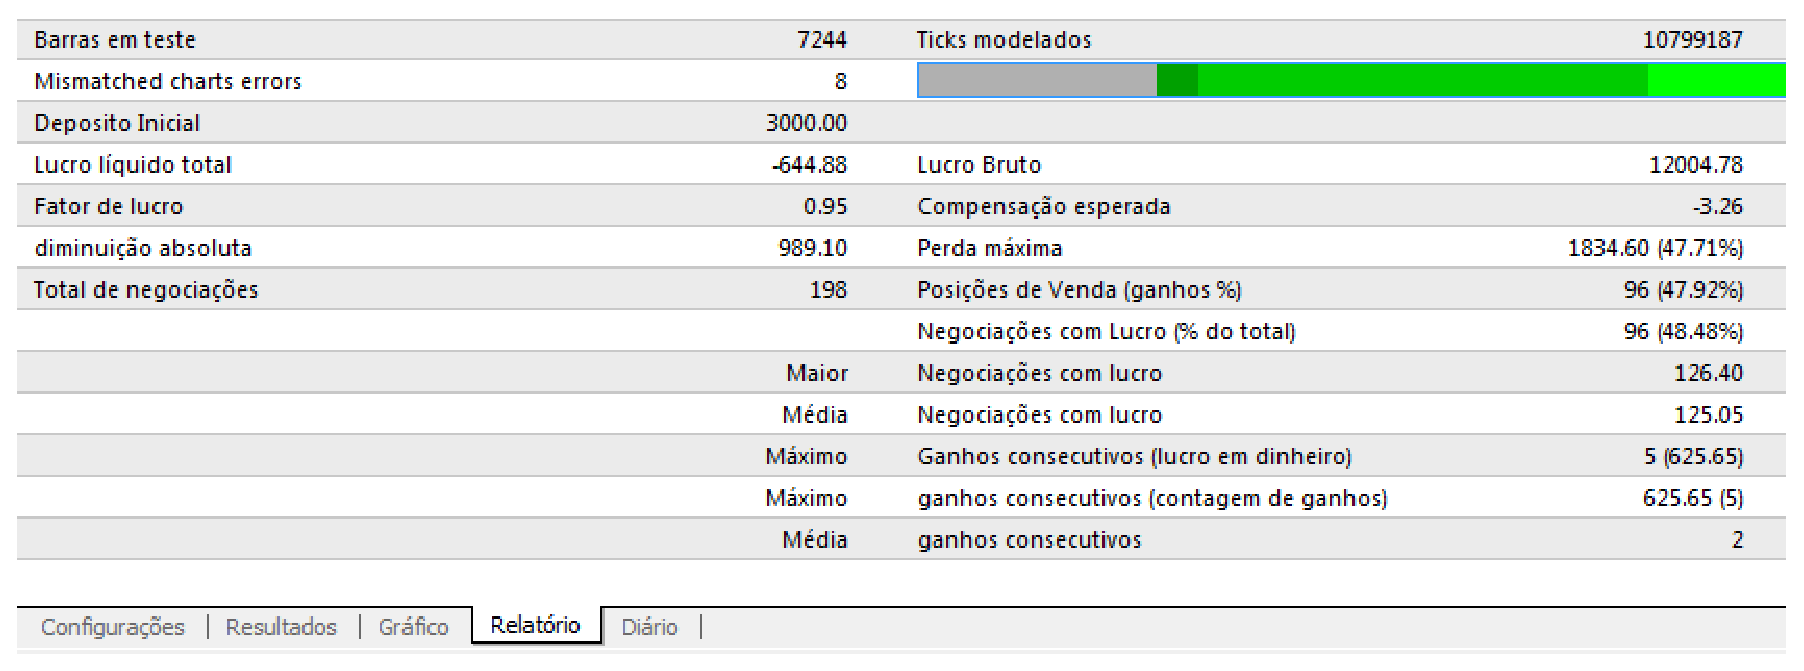
\includegraphics[width=0.9\textwidth]{figuras/protocoloMedia2}
\caption{Relatório de simulação no período de Agosto de 2013 a Agosto de 2014 do \textit{expert} MediaMovel.mql} 
\label{protocoloMedia2}
\end{figure}

É possível visualizar nos gráficos das simulações, as perdas de capital que o \textit{expert} MediaMovel.mql gerou.

\begin{figure}[H]
\centering
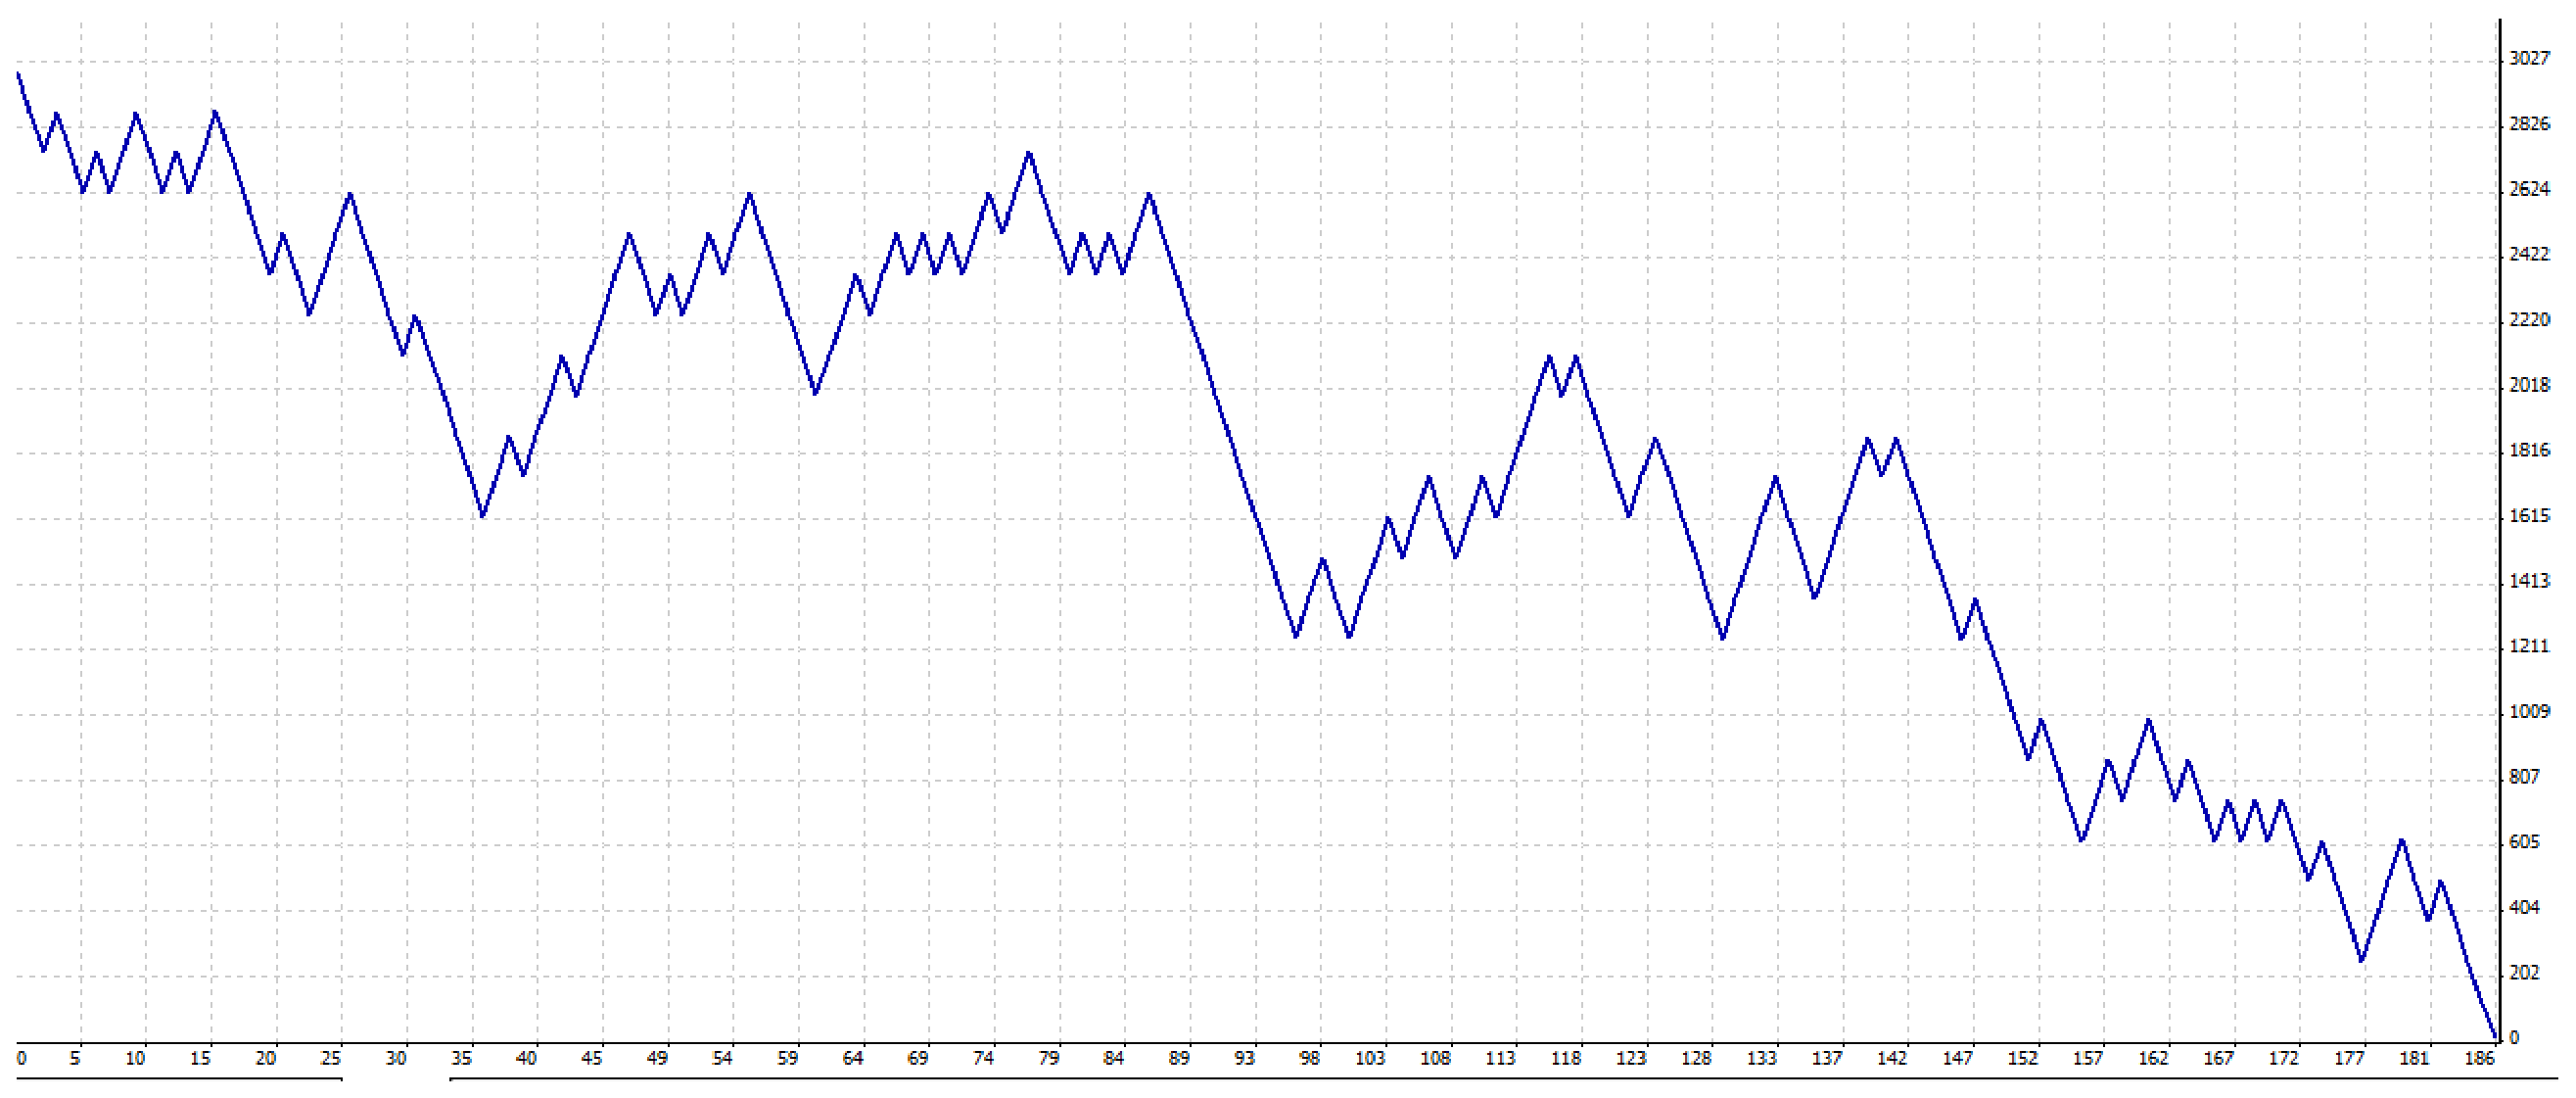
\includegraphics[width=0.9\textwidth]{figuras/protocoloMedia3}
\caption{ Gráfico gerado pela simulação do \textit{expert} MediaMovel.mql no período de Agosto de 2012 a Agosto de 2013} 
\label{protocoloMedia3}
\end{figure}

\begin{figure}[H]
\centering
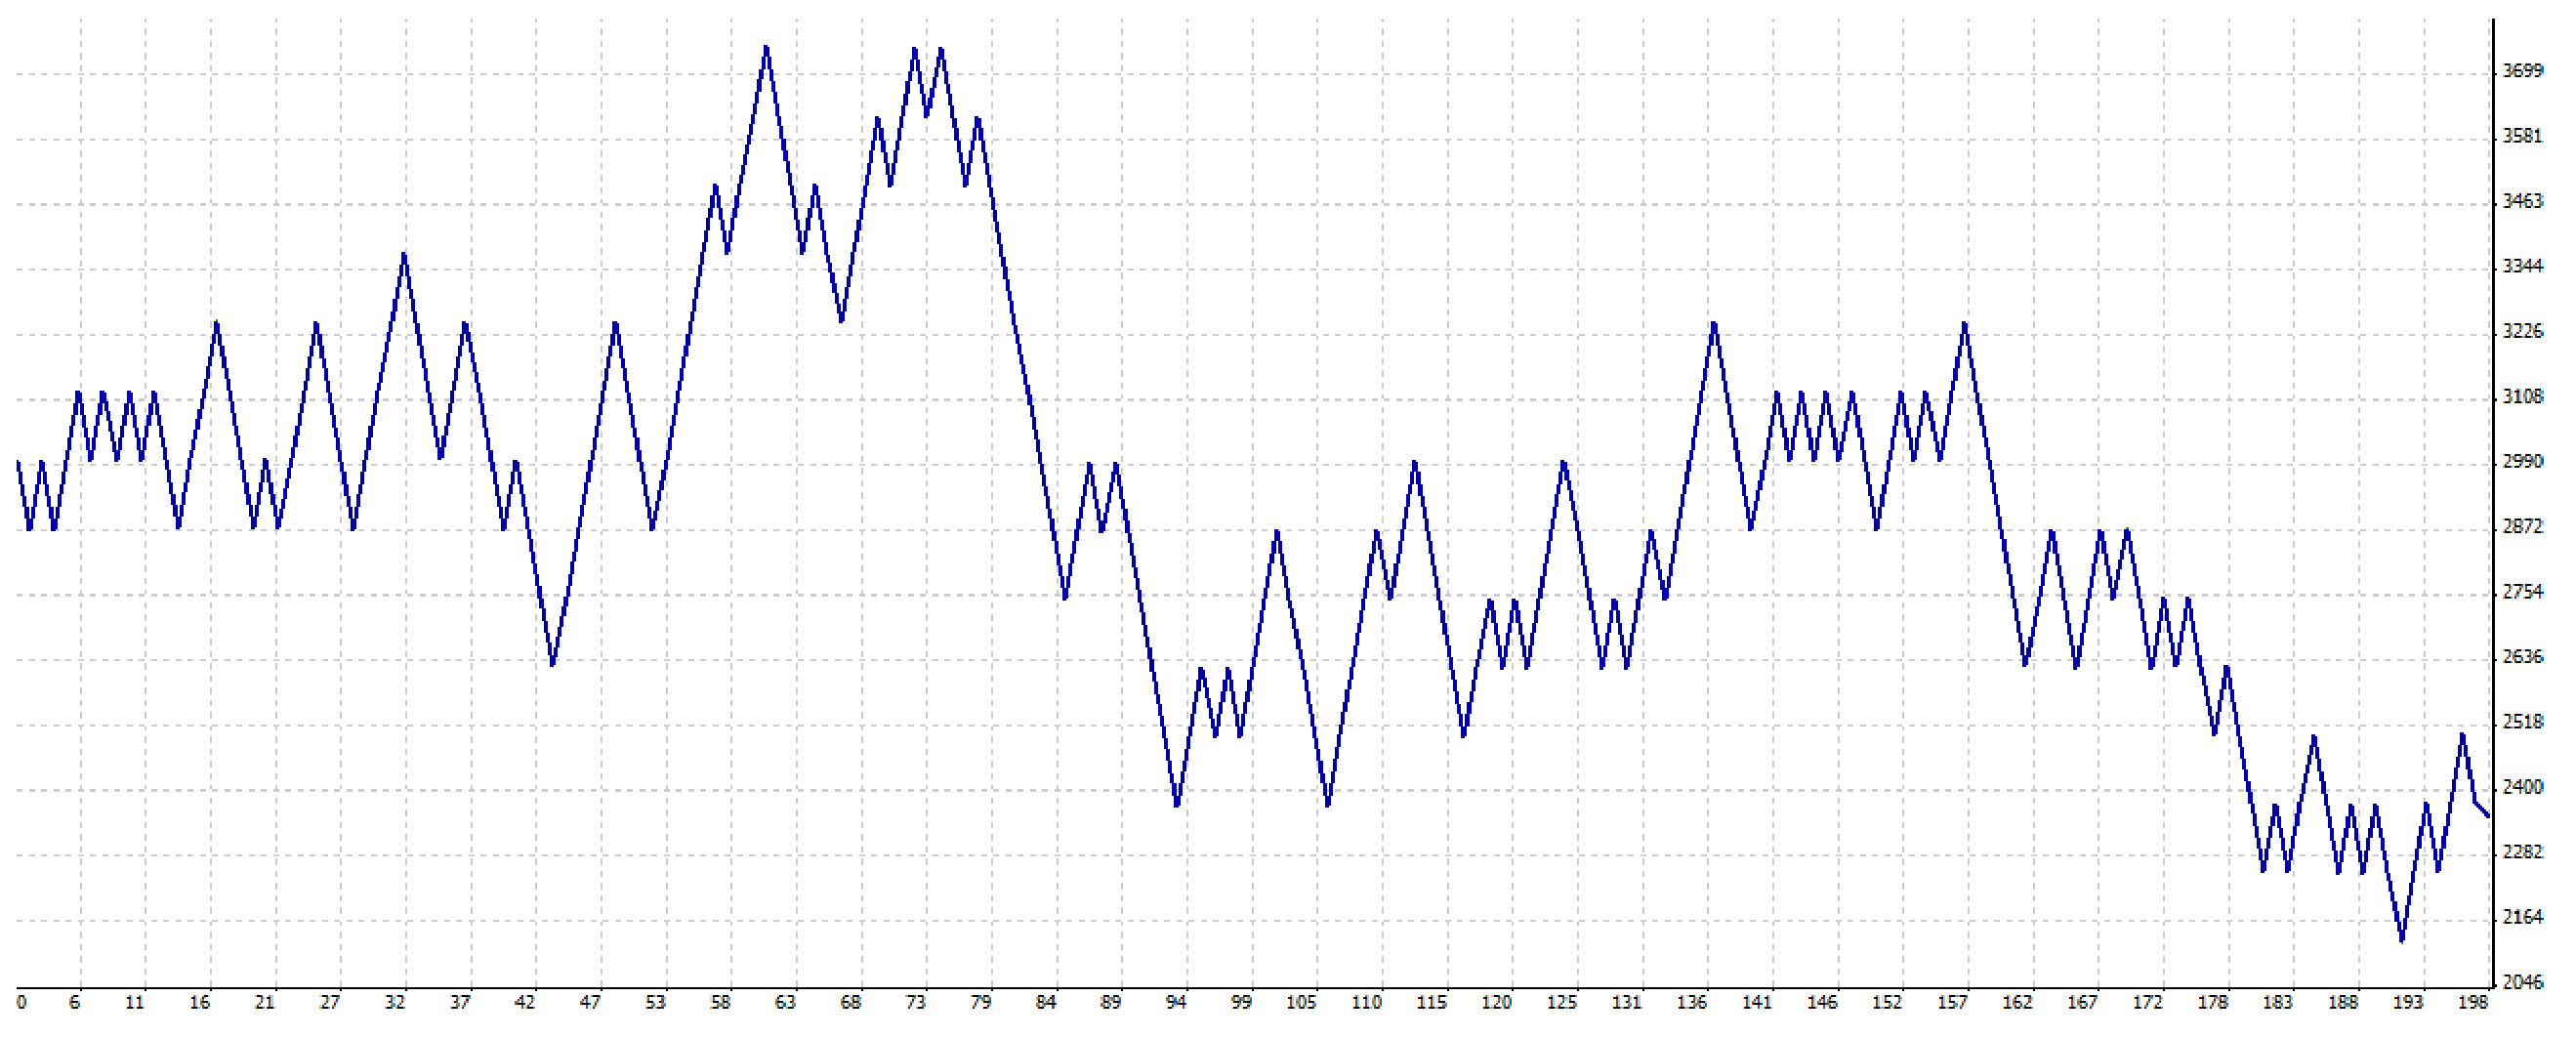
\includegraphics[width=0.9\textwidth]{figuras/protocoloMedia4}
\caption{ Gráfico gerado pela simulação do \textit{expert} MediaMovel.mql no período de Agosto de 2013 a Agosto de 2014} 
\label{protocoloMedia4}
\end{figure}


\subsection{Definição métodos de operação ferramenta InvestMVC}

Os métodos matemáticos de Correlação Linear, Fibonacci e Mínimos Quadrados tiveram êxito nos dois anos de simulação (agosto 2012 a agosto de 2014). Os métodos de Estocástico e Média Móvel tiveram prejuízo nos dois anos de simulação. Portanto, foram escolhidos os métodos de Correlação Linear, Fibonacci e Mínimos Quadrados como métodos de estratégia financeira do software InvestMVC.

\section{Arquitetura InvestMVC}

Arquitetura Orientada a Componentes possui o propósito de dividir para conquistar. Um grande problema é quebrado em partes menores e em seguida se desenvolve soluções mais elaboradas \cite{john}.

Por usar vários paradigmas, a ferramenta InvestMVC terá vários componentes e cada componente terá seu paradigma de programação e responsabilidade bem definida, como mostrado na Figura \ref{componente}.

\begin{figure}[H]
\centering
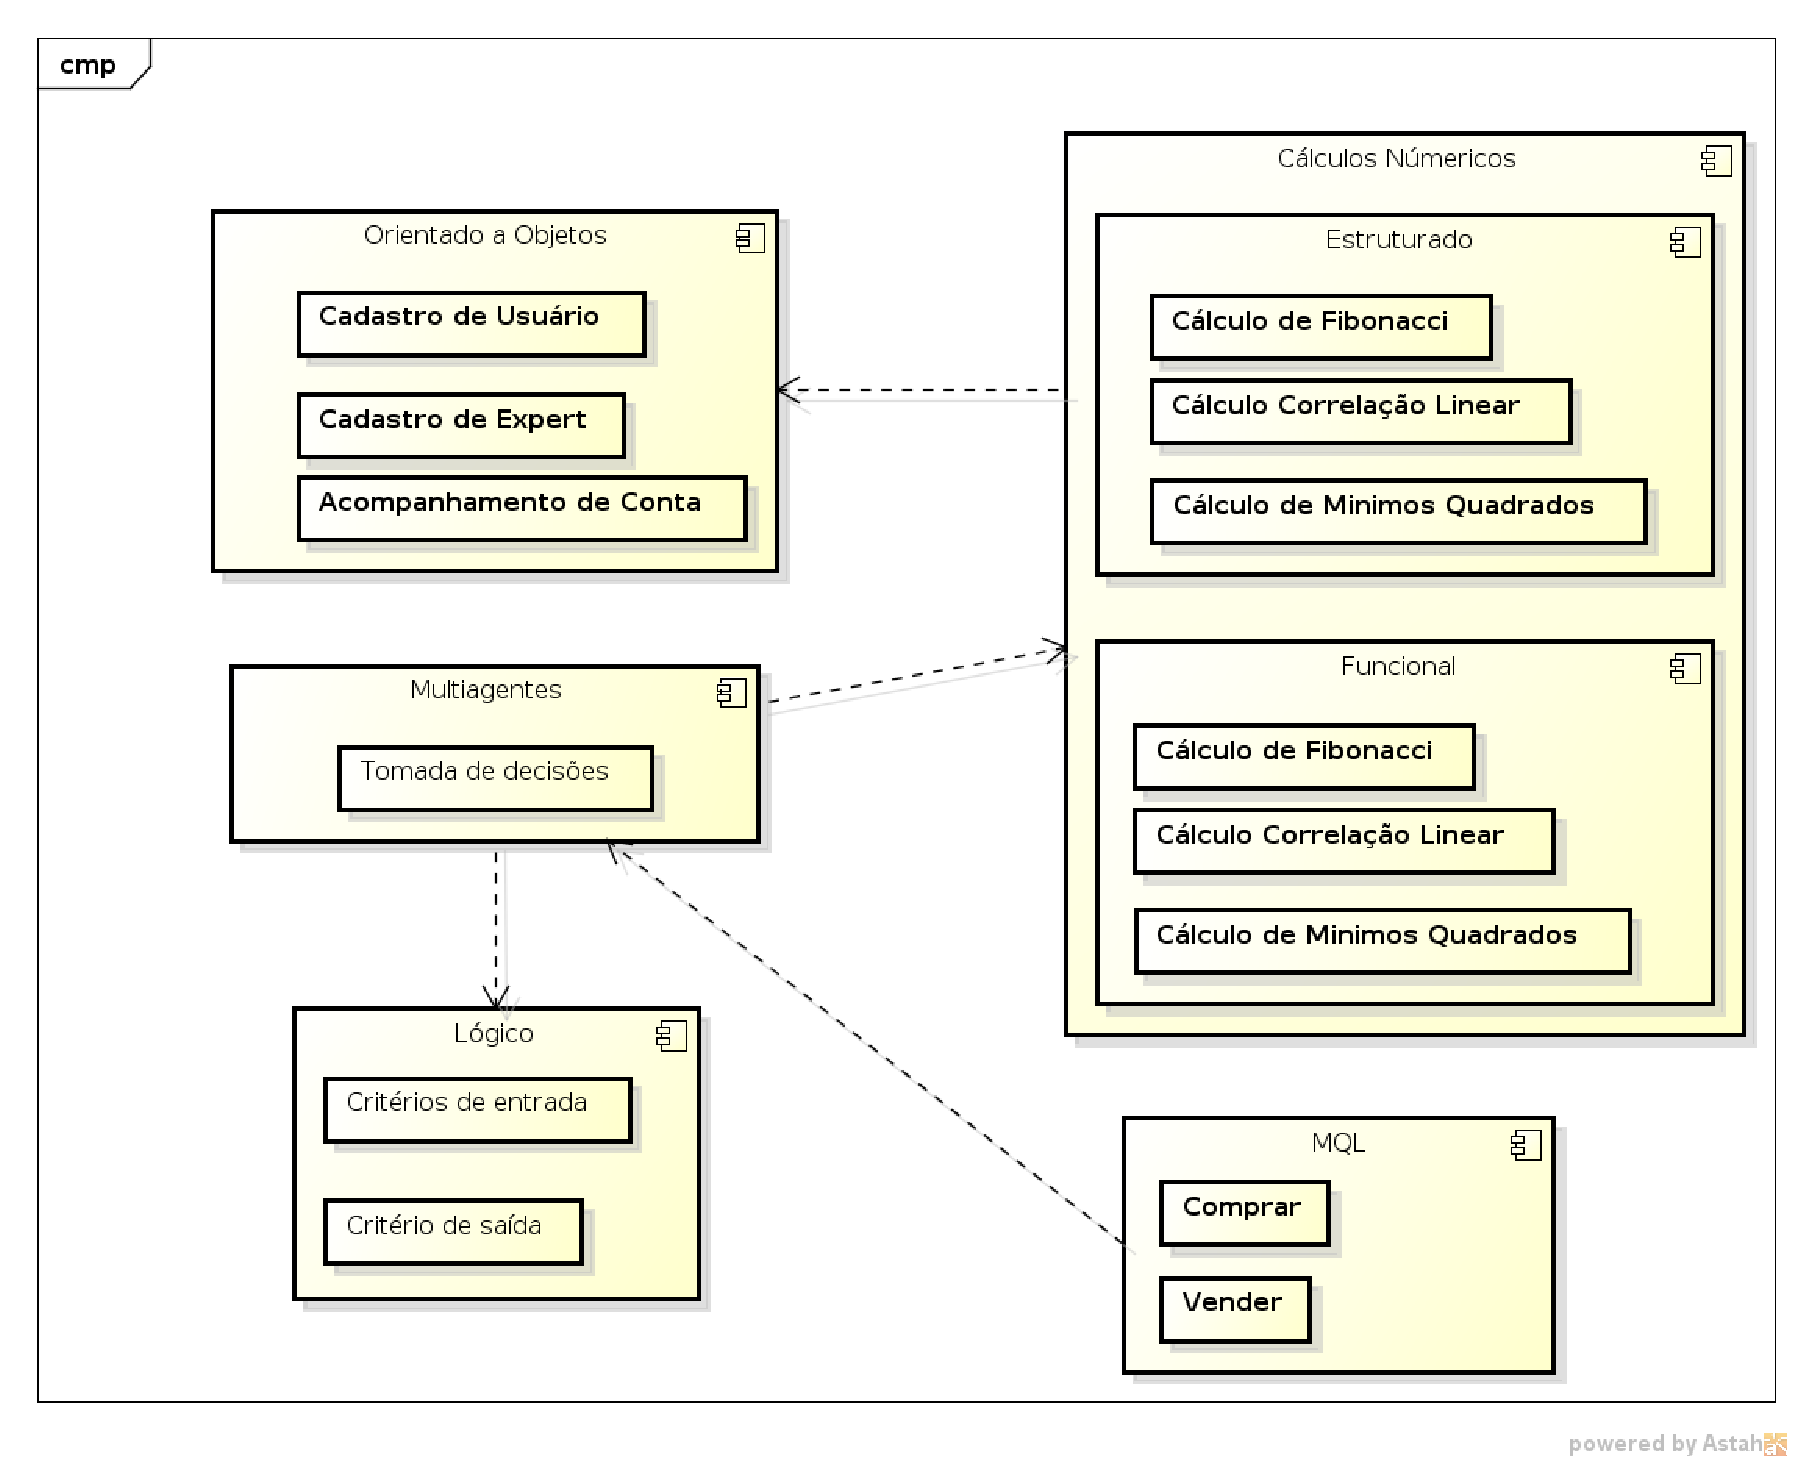
\includegraphics[width=0.9\textwidth]{figuras/componente}
\caption{Diagrama de Sequência InvestMVC}
\label{componente}
\end{figure}

\subsection{Componente Orientado a Objetos}

Este componente faz a interação com o usuário e foi implementado em linguagem Groovy. A escolha dessa linguagem, se deu porque esta é voltada para aplicações web e juntamente com  o framework grails, fornece a criação de um projeto com uma arquitetura MVC definida, como demonstra a Figura \ref{classeOO}.

\begin{figure}[H]
\centering
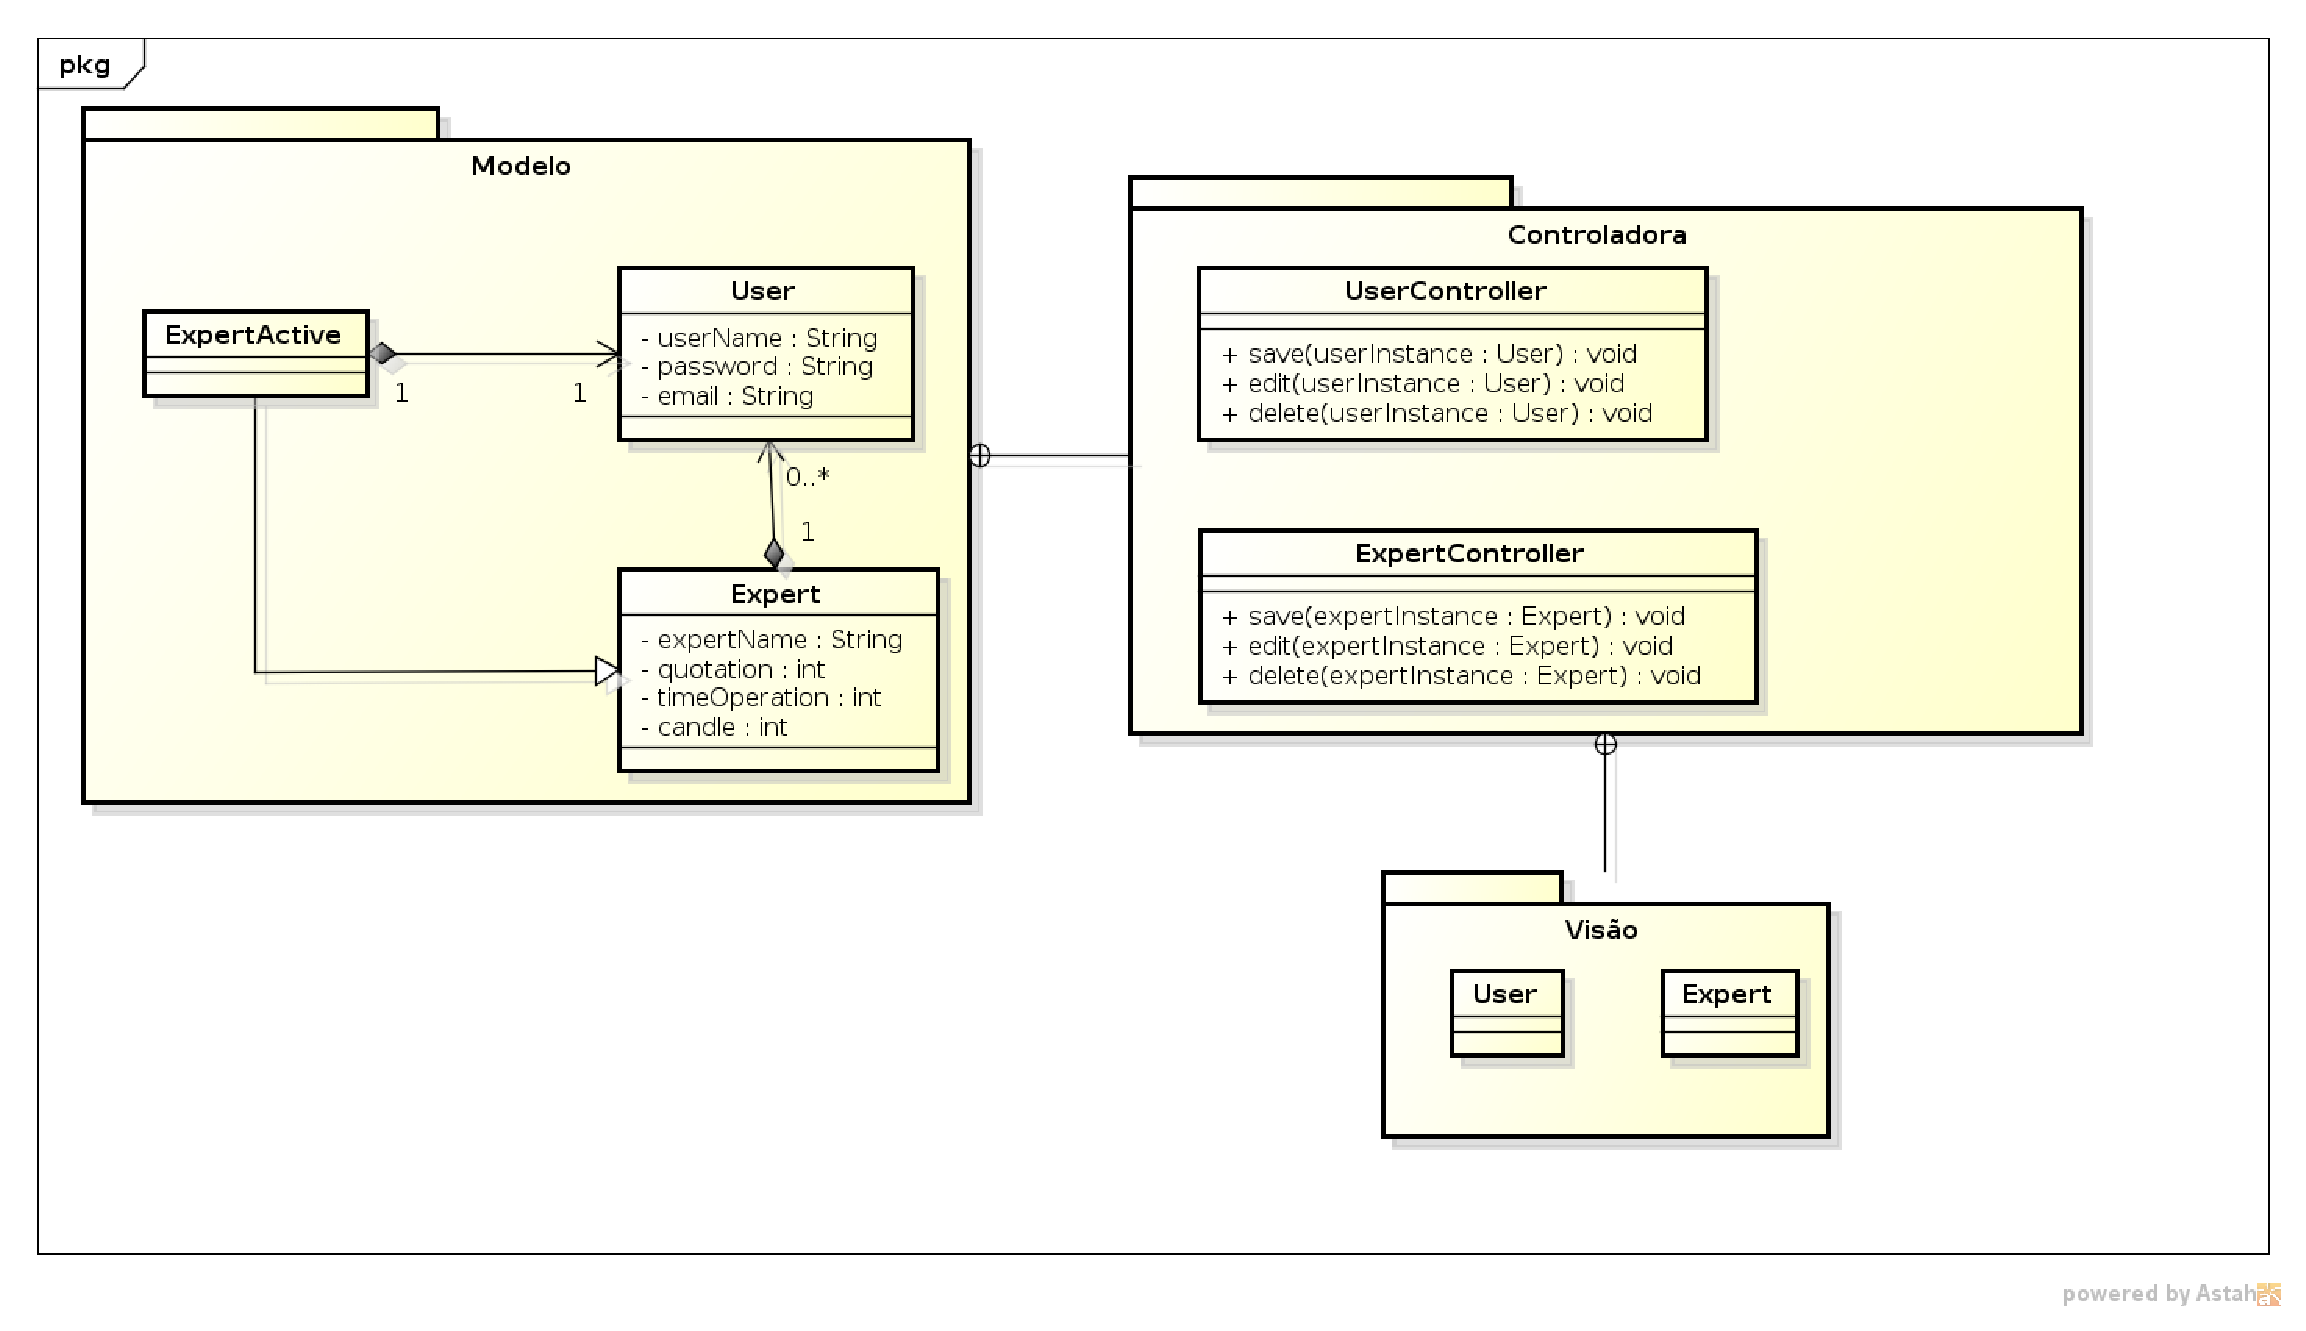
\includegraphics[width=0.9\textwidth]{figuras/classeOO}
\caption{Diagrama de Classe InvestMVC componente Orientado a Objetos} 
\label{classeOO}
\end{figure}

Segundo \citeonline{lamin} na arquitetura MVC o controle de fluxo de dados dentro deste módulo ocorre da seguinte forma:

\begin{enumerate}
\item O usuário,neste caso o investidor, interage com a Visão.
\item A Controladora manipula o evento da interface do usuário através de uma rotina.
\item A Controladora acessa o Model, atualizando-o baseado na interação do usuário.
\end{enumerate}

O diagrama de sequência do componente Orientado a Objetos é evidenciado na Figura \ref{sequenciaOO}.

\begin{figure}[H]
\centering
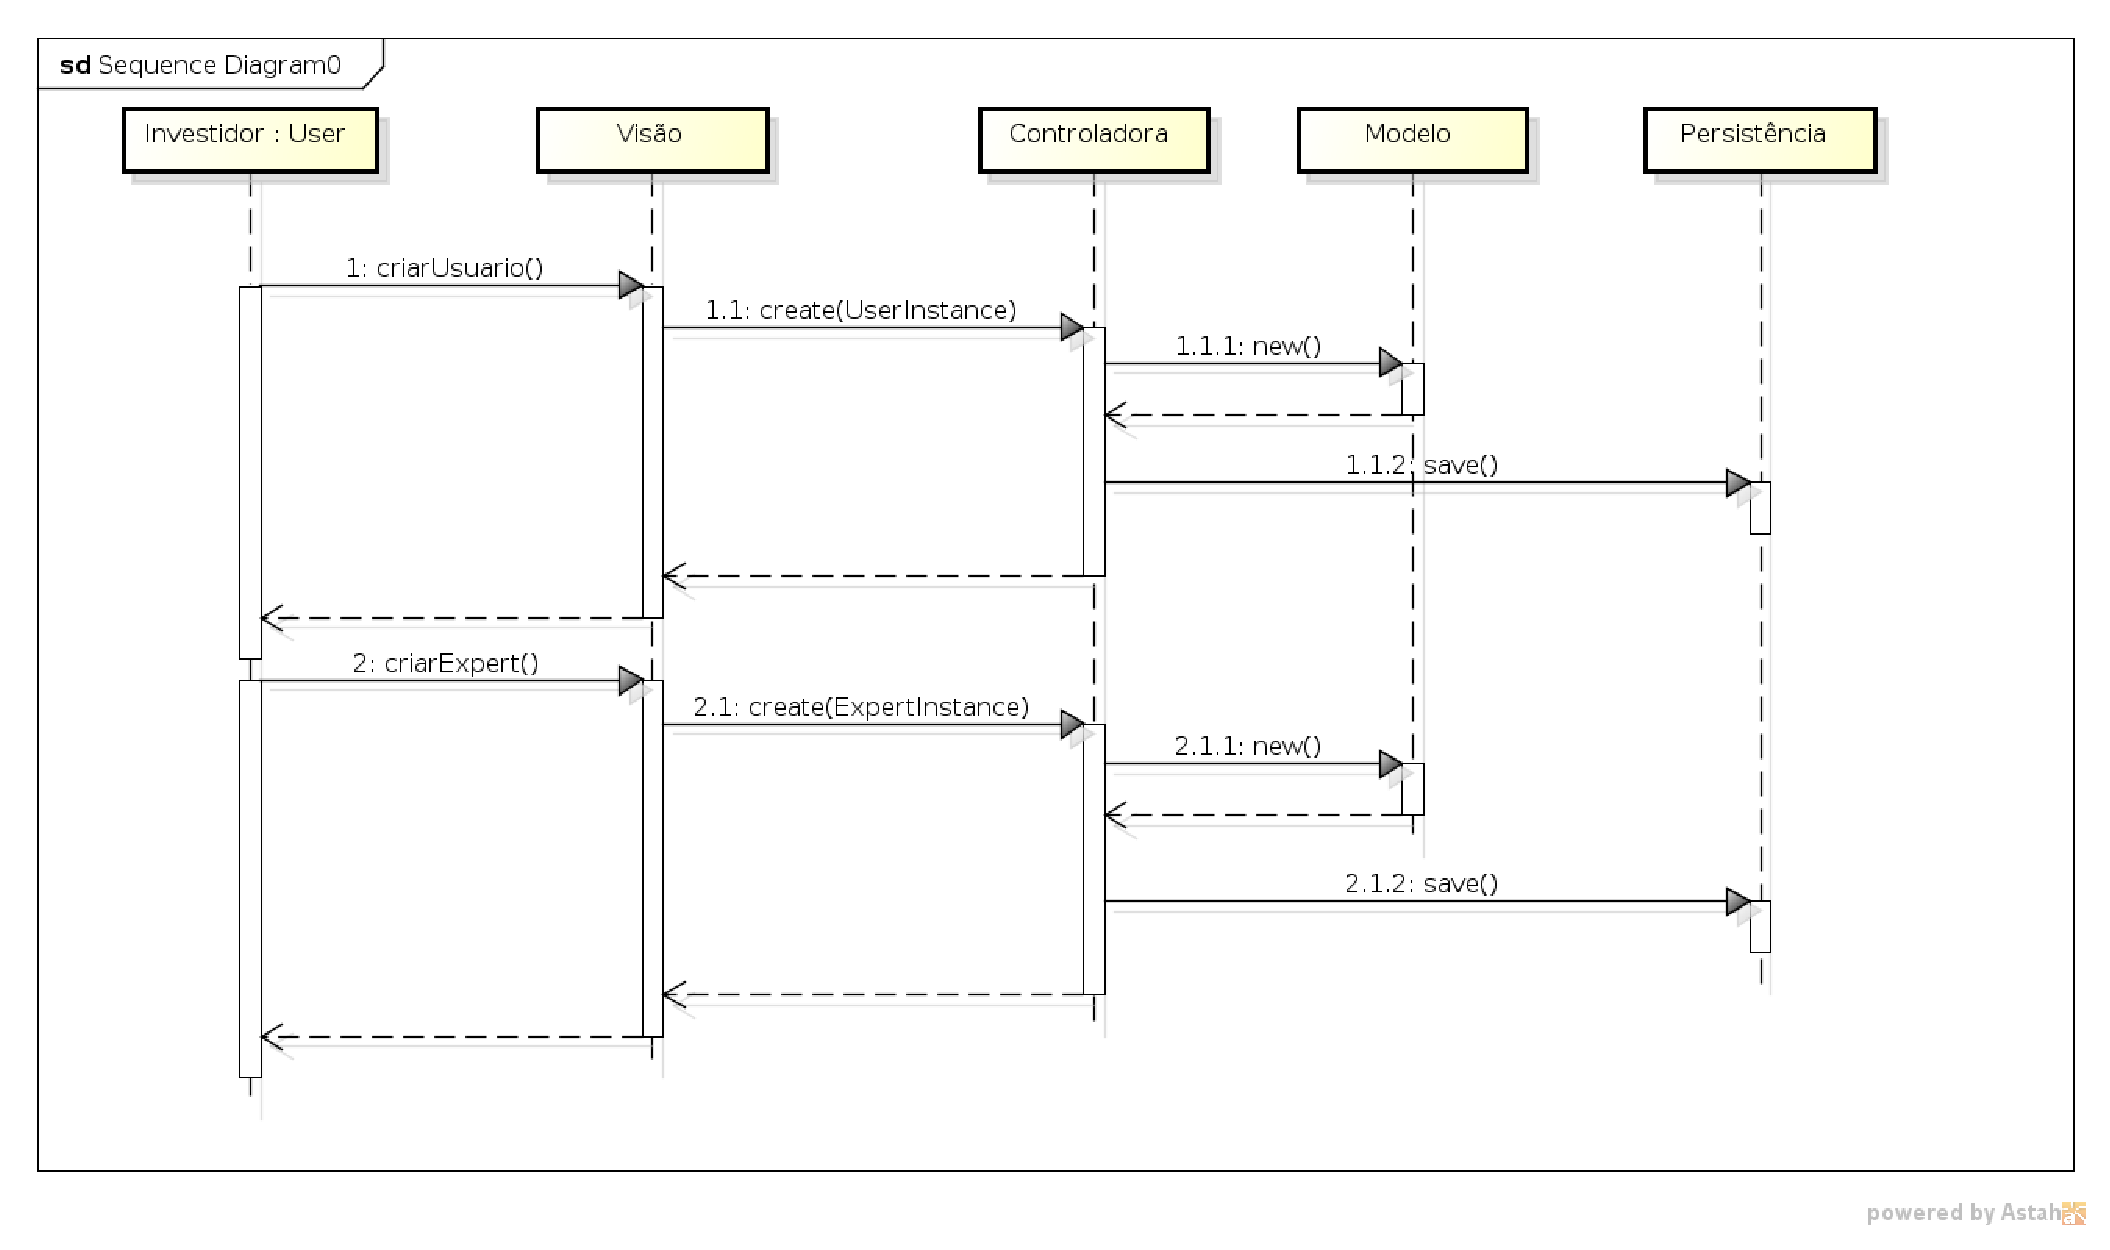
\includegraphics[width=0.9\textwidth]{figuras/sequenciaOO}
\caption{Diagrama de sequência InvestMVC componente Orientado a Objetos}
\label{sequenciaOO}
\end{figure}

\subsection{Componente Cálculos Numéricos}

O componente Cálculos Numéricos é responsável por calcular os métodos matemáticos presentes na ferramenta InvestMVC. Este módulo é composto por dois outros módulos: módulo Estruturado e módulo Funcional.

O componente Estruturado da ferramenta InvestMVC foi programado em linguagem C e o módulo Funcional em linguagem Haskell. Ambos os componentes realizam os mesmos cálculos. Isso aumenta a probabilidade de não ocorrer erros nos cálculos dos métodos matemáticos. Caso um dos componentes por algum motivo não seja executado no momento correto, a tendência é que o outro módulo realize os cálculos.

\subsubsection{Componente Funcional}
A linguagem Haskell por ser uma linguagem de programação funcional sua "gramática" está próxima das funções matemáticas, logo a implementação dos métodos algébricos e numéricos se torna muito intuitiva. \cite{hoogle2013}.

O paradigma funcional é declarativo, por limitar o uso de atribuições à variáveis suas funções são mais precisas do que em outros paradigmas \cite{piponi2006}.

Devido aos fatos externalizados, o paradigma funcional, foi utilizado para implementar os métodos matemáticos de Correlação Linear, Mínimos Quadrados e Fibonacci. Por ser simples, este componente será formado apenas por seus 4 arquivos haskell, cada arquivo realiza o cálculo de um método matemático, com execeção do arquivo  Arquivos.hs, que faz a leitura de arquivos.

\begin{figure}[H]
\centering
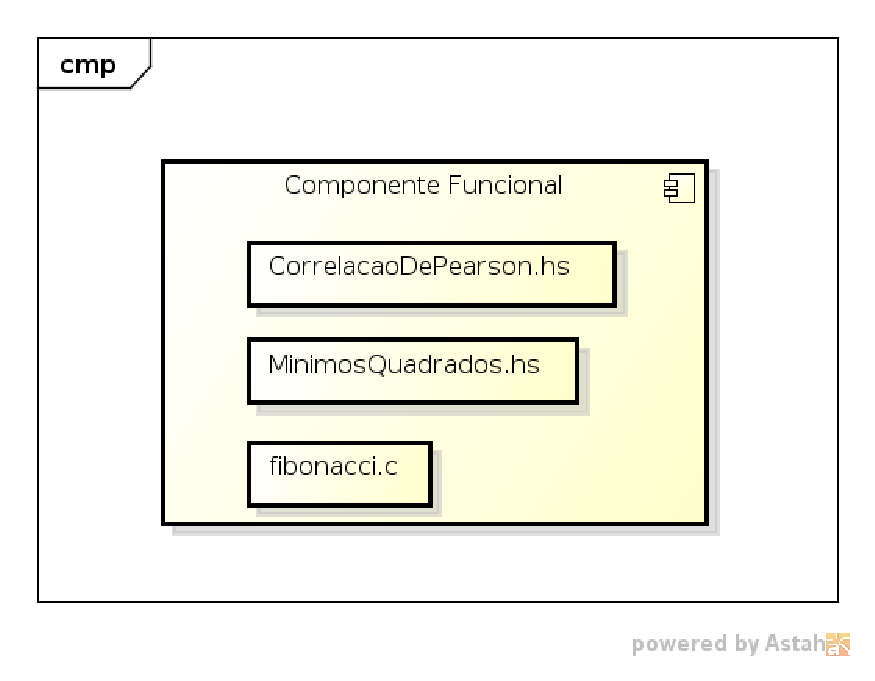
\includegraphics[width=0.5\textwidth]{figuras/componenteFuncional}
\caption{Componente Funcional InvestMVC} 
\label{componenteFuncional}
\end{figure}

O componente Funcional espera uma socilitação de cálculo do componente Multiagente, logo após a solicitação o componente busca na persistência (um arquivo) as cotações do mercado, com estas cotações o componente é capaz de realizar o cálculo do método matemático que é esperado pelo componente Multiagente, como é mostrado na Figura \ref{sequenciaFuncional}.

\begin{figure}[H]
\centering
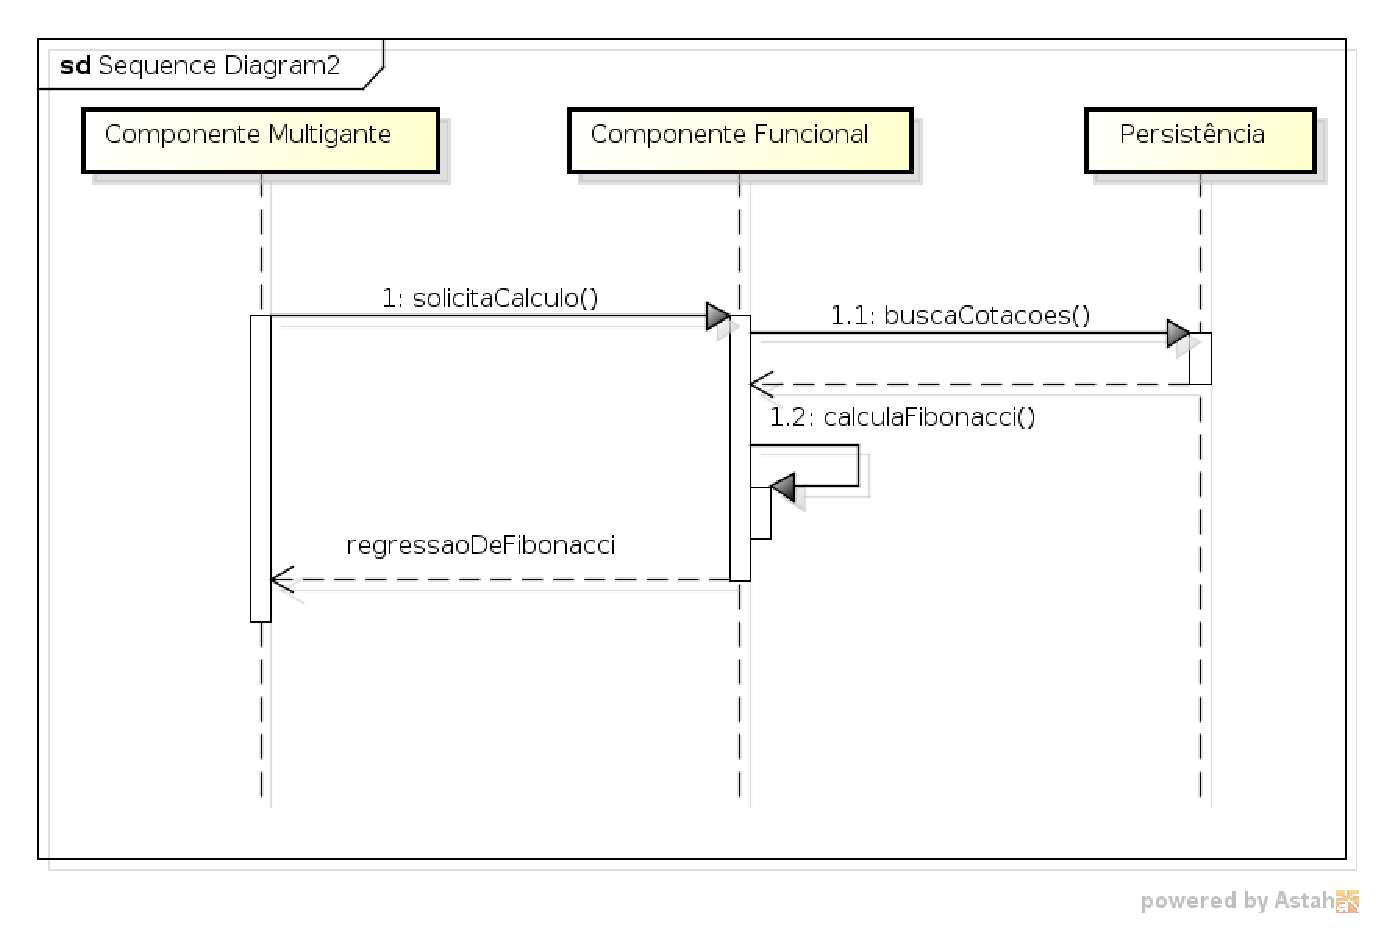
\includegraphics[width=0.9\textwidth]{figuras/sequenciaFuncional}
\caption{Diagrama de Sequência do Componente Funcional InvestMVC} 
\label{sequenciaFuncional}
\end{figure}

\subsubsection{Componente Estruturado}

A linguagem de programação C é estruturada e possui a vantagem da velocidade de execução do código fonte. Também é uma linguagem bastante utilizada para realizar cálculos numéricos e algébricos \cite{gustavo}. 

O paradigma estruturado utilizando a linguagem C, também foi utilizado para implementar os métodos matemáticos de Correlação Linear, Mínimos Quadrados e Fibonacci.

A arquitetura e sequência do fluxo de dados do Componente Estruturado segue a mesma lógica do Componente Funcional, como ilustrado na Figura \ref{sequenciaEstruturado}.

\begin{figure}[H]
\centering
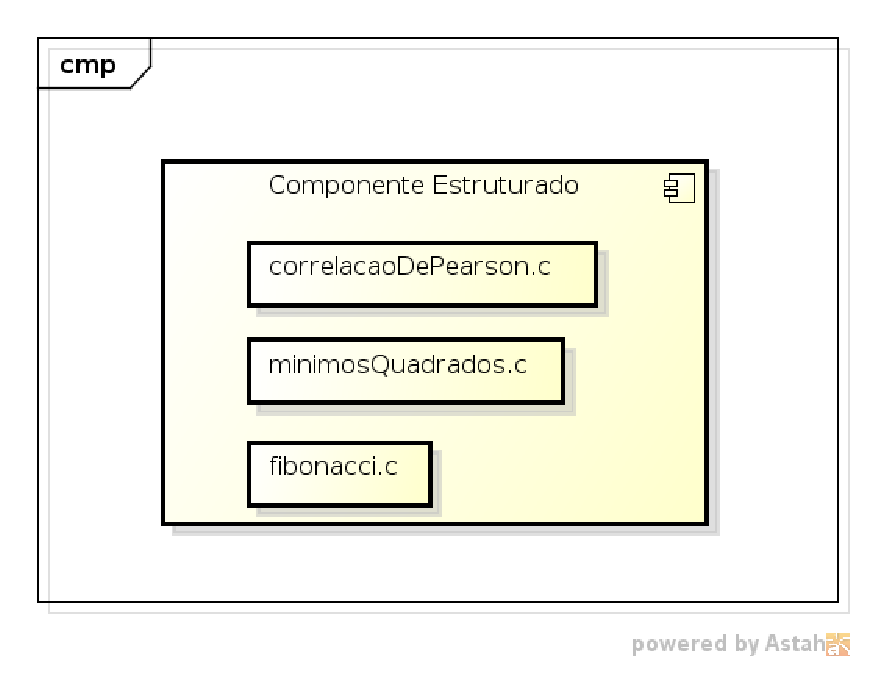
\includegraphics[width=0.7\textwidth]{figuras/componenteEstruturado}
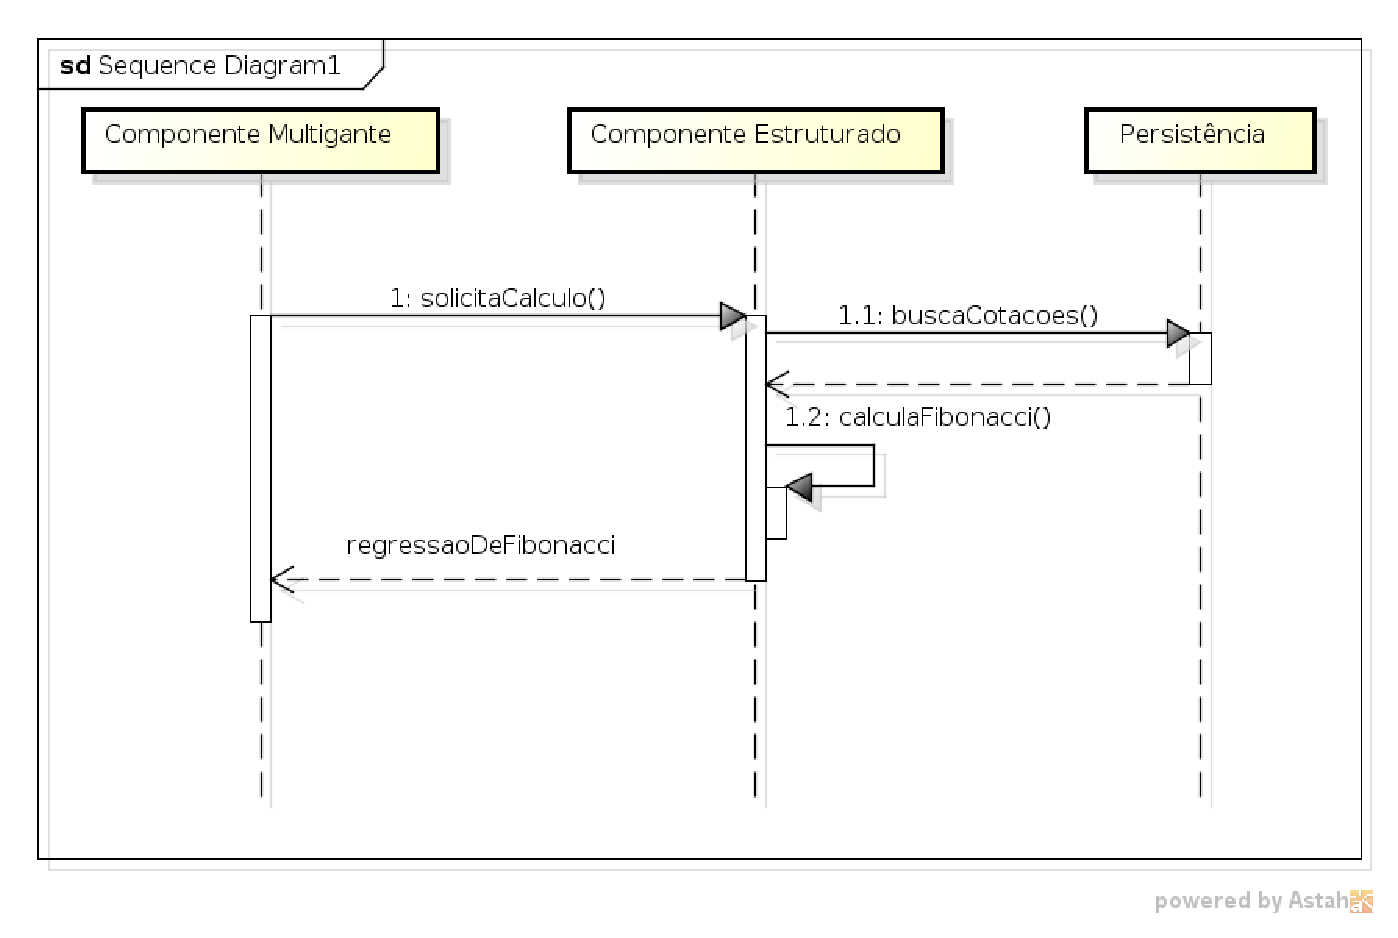
\includegraphics[width=0.7\textwidth]{figuras/sequenciaEstruturado}
\caption{Diagramas de Componentes e de Sequência do Componente Estruturado InvestMVC.}
\label{sequenciaEstruturado}
\end{figure}

\subsection{Componente Multiagente}

O componente Multiagente foi implementado usando o paradigma Multiagente com a linguagem Java. 

Agentes de software são entidades autônomas e com capacidades sociais, o uso deste paradigma justifica-se na tomada de decisões \cite{agentBuilderWhy}. 

Os agentes da ferramenta  InvestMVC possuem uma arquitetura reativa, pois suas ações se dão pelas variações que ocorrem nas cotações do Mercado de Moedas.

A arquitetura do Componente Multiagente está modularizada por pacotes: o pacote comportamentos é formado por compormentos que são usados pelos Agentes de Software, o pacote metodos matemáticos é formado por Agentes que acessam o componente Cálculos matemáticos, o pacote investidores é composto por agentes que interagem com o Componente MQL e o pacote execucao inicia a execução do SMA.

\begin{figure}[H]
\centering
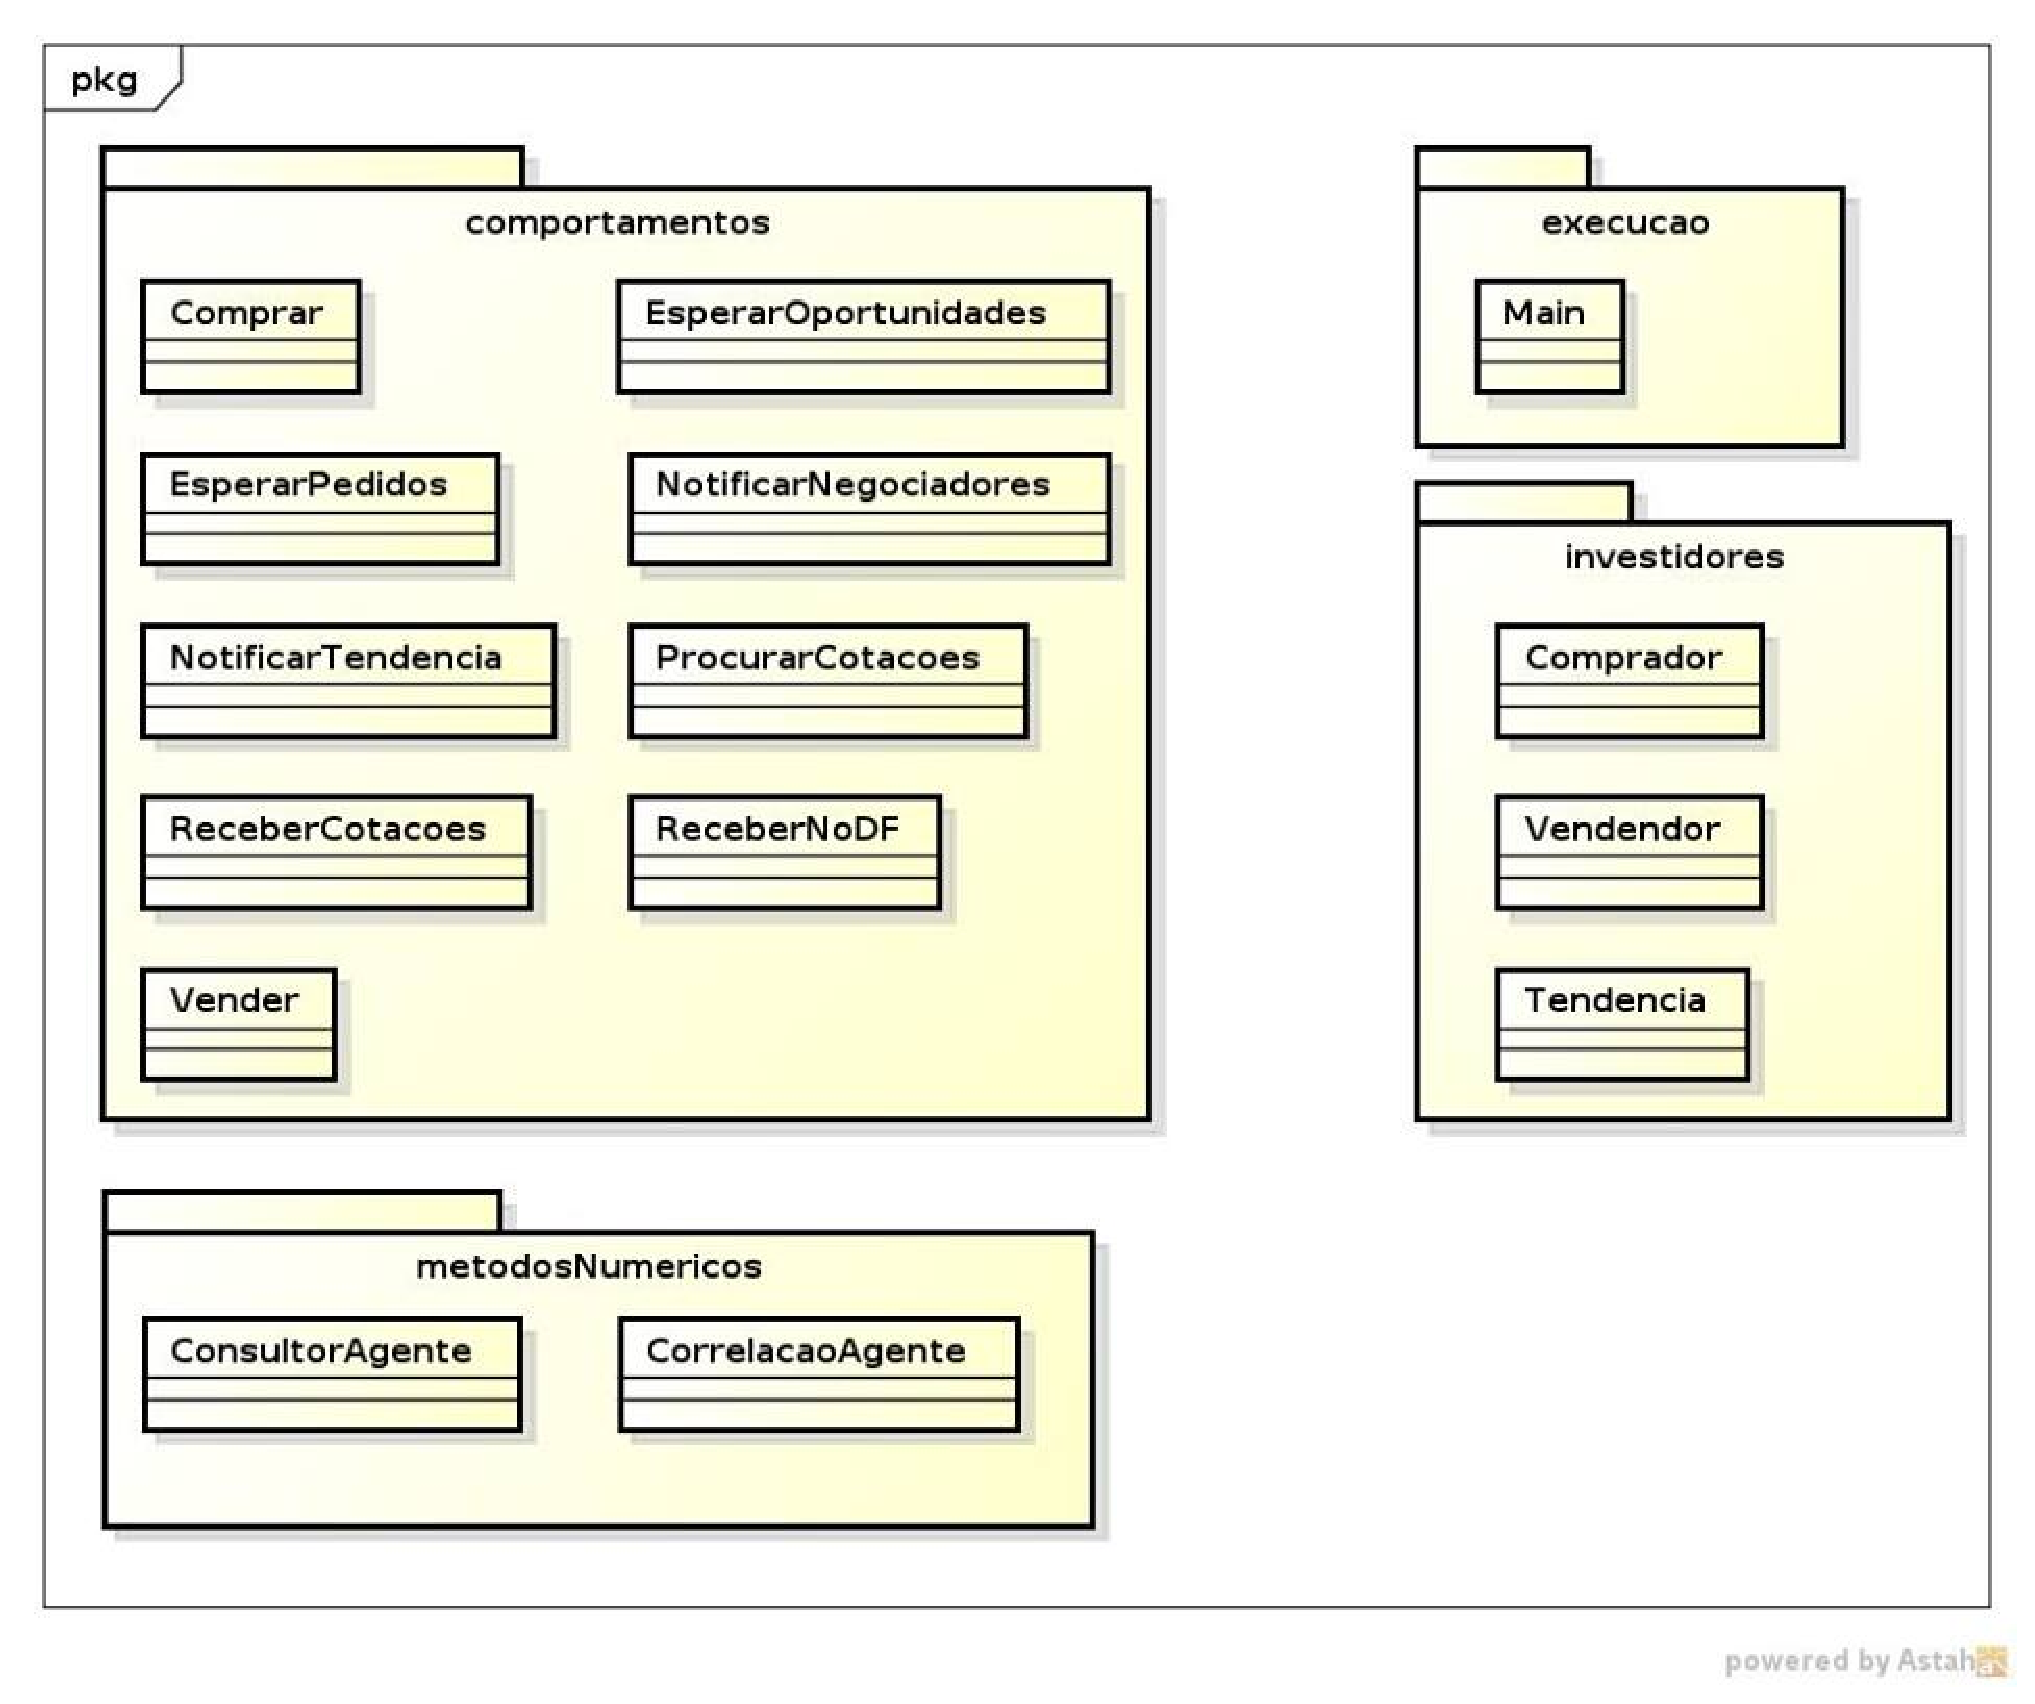
\includegraphics[width=0.9\textwidth]{figuras/diagramaClassesSMA}
\caption{Diagrama de Classe do Componente Multiagente InvestMVC} 
\label{diagramaClassesSMA}
\end{figure}

\subsection{Componente Lógico}

O componente Lógico foi produzido em linguagem Prolog e definiu uma base de conhecimento que serve como critério de entrada e saída no Mercado de Moedas.

O paradigma Lógico facilita a representação, inserção e recuperação de conhecimento, por isso é muito usado em aplicações com Inteligência Artificial \cite{almeida2010}.

A interação do Componente Lógico com o Componente Multiagentes é evidenciada na Figura \ref{sequenciaLogico}.

\begin{figure}[H]
\centering
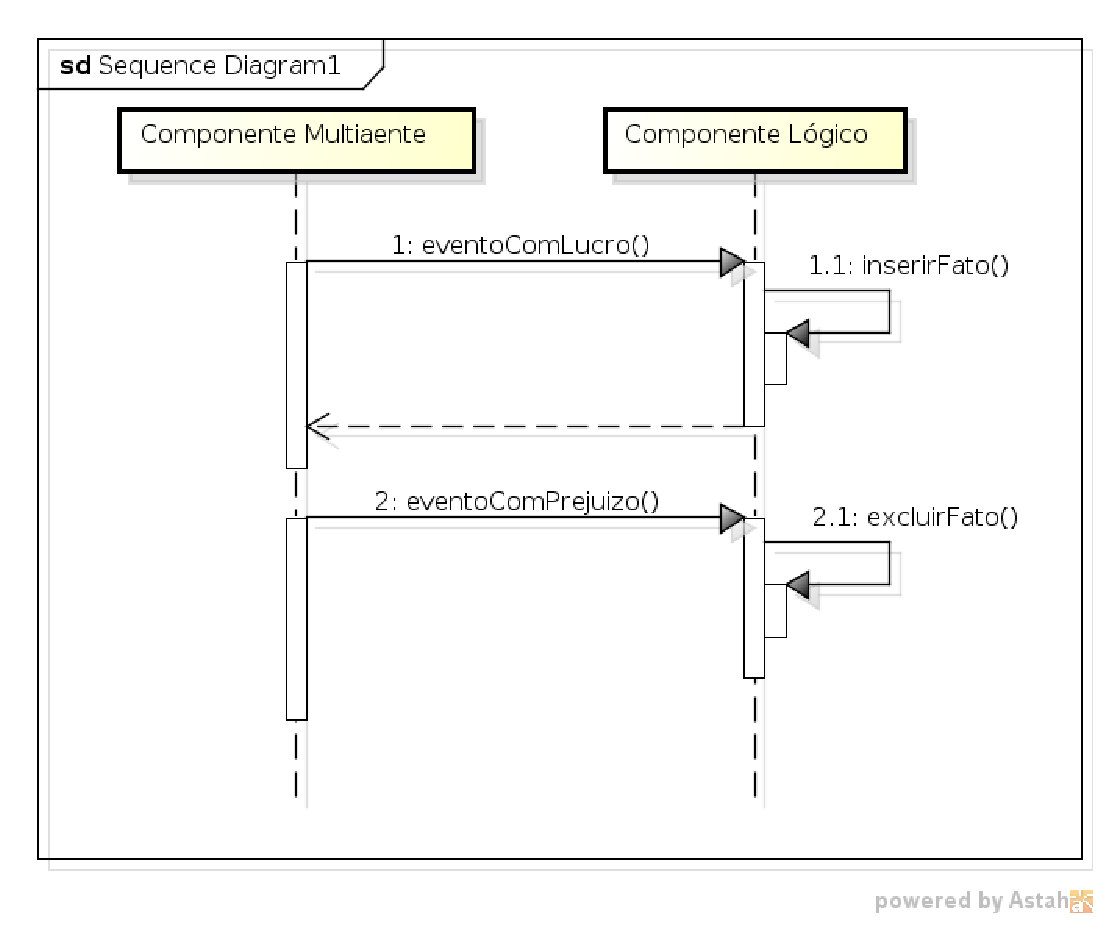
\includegraphics[width=0.7\textwidth]{figuras/sequenciaLogico}
\caption{Diagrama de Sequência do Componente Lógico InvestMVC.}
\label{sequenciaLogico}
\end{figure}

\subsection{Componente MQL}

O componente MQL é responsável por receber a resposta do Componente Multiagentes para realizar uma compra ou venda. Também é recebido outros atributos relacionados a compra ou venda, como alavancagem, stop loss e take profit.

A interação do Componente MQL com o Componente Multiagentes é evidenciada na Figura \ref{sequenciaMQL}.

\begin{figure}[H]
\centering
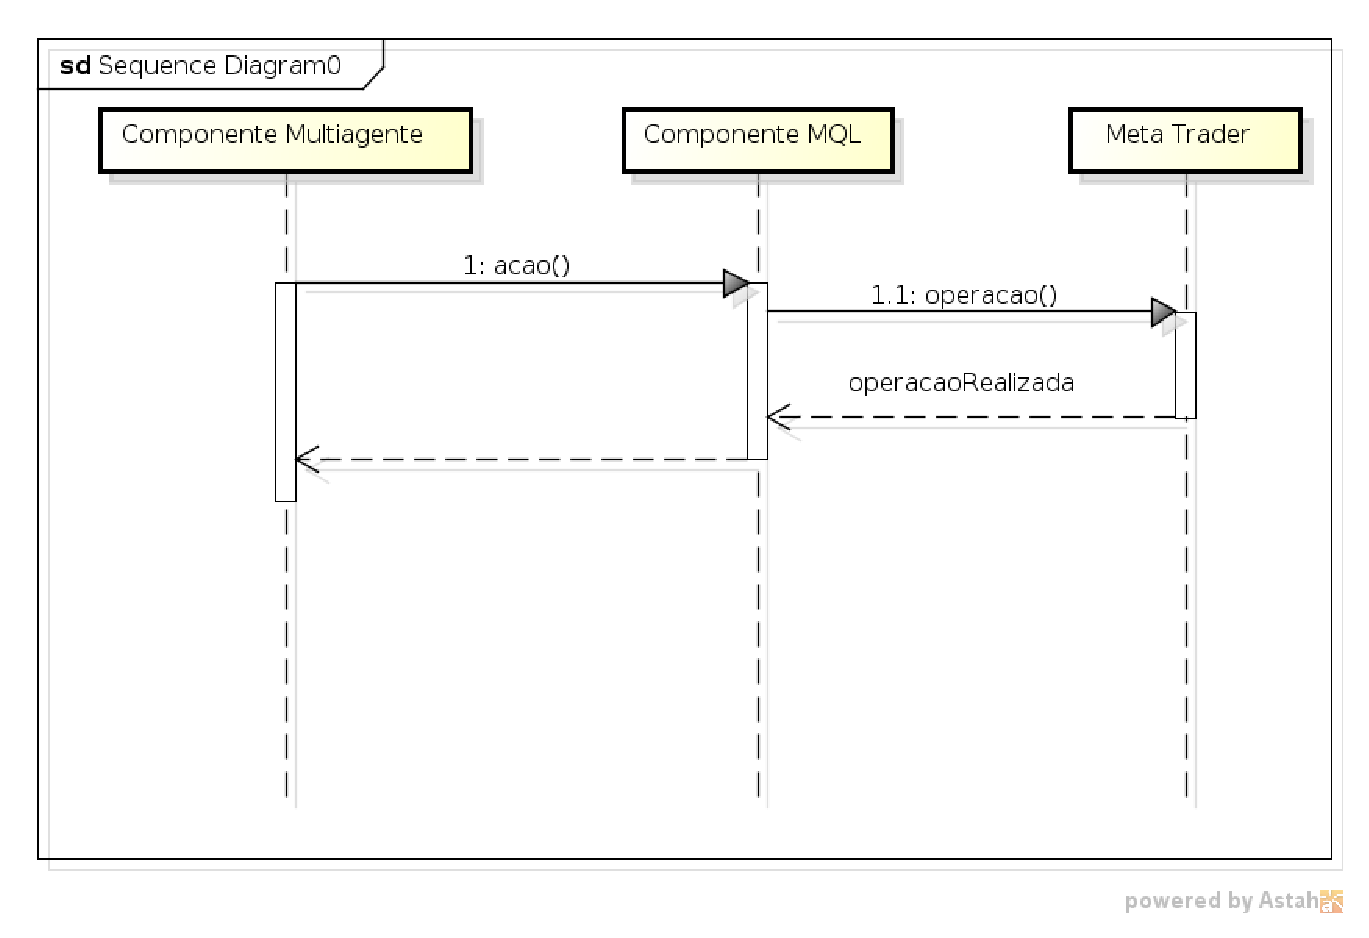
\includegraphics[width=0.5\textwidth]{figuras/sequenciaMQL}
\caption{Diagrama de Sequência do Componente MQL InvestMVC.}
\label{sequenciaMQL}
\end{figure}


\section{Testes unitários}

\subsection{Componente Funcional}

Foram realizados os testes unitários na linguagem haskell utilizando o framework HUnit. O framework não fornece a cobertura de código fonte, mas é possível visualizar a quantidade de casos de teste, quantidade de testes realizados, quantidade de erros e quantidade de falhas. Os resultados dos testes unitários dos métodos de Correlação de Pearson, Fibonacci e Mínimos Quadrados podem ser visualizados na Figura \ref{testeCorrelacaoHaskell}, \ref{testeFibonacciHaskell} e \ref{TesteMinimosHaskell}.

\begin{figure}[H]
\centering
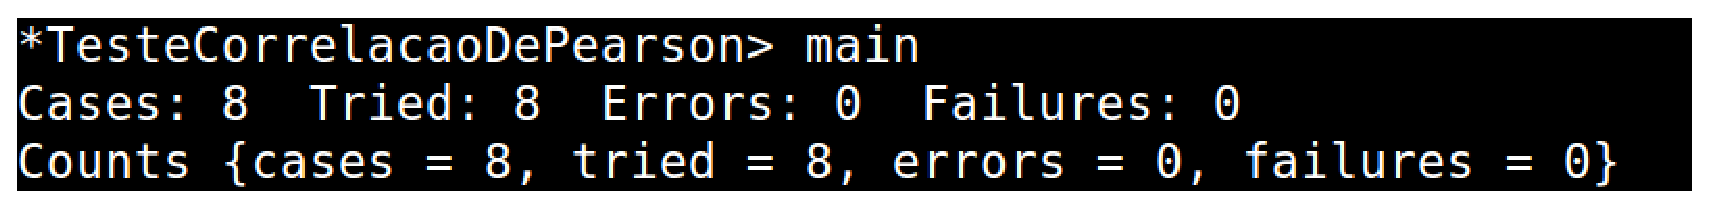
\includegraphics[width=0.9\textwidth]{figuras/testeCorrelacaoHaskell}
\caption{Resultado da Suíte de Teste do Método Correlação Linear}
\label{testeCorrelacaoHaskell}
\end{figure}

\begin{figure}[H]
\centering
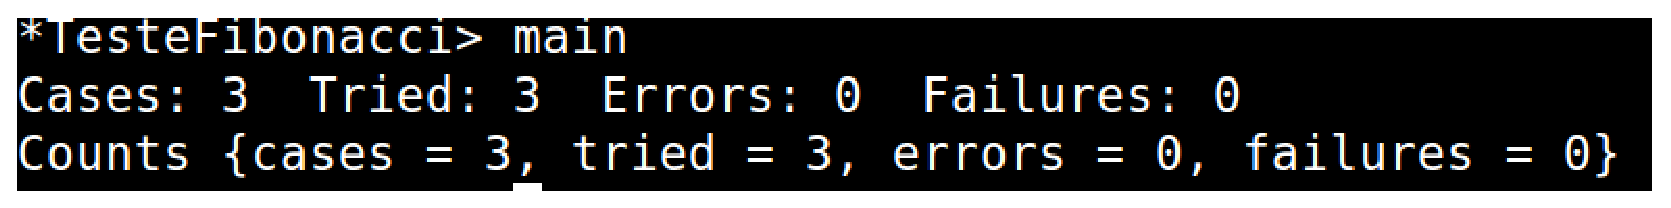
\includegraphics[width=0.9\textwidth]{figuras/testeFibonacciHaskell}
\caption{Resultado da Suíte de Teste do Método de Fibonacci}
\label{testeFibonacciHaskell}
\end{figure}

\begin{figure}[H]
\centering
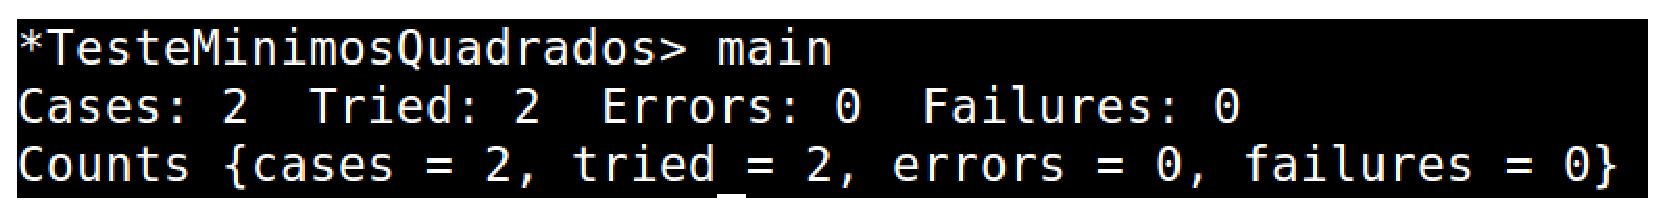
\includegraphics[width=0.9\textwidth]{figuras/TesteMinimosHaskell}
\caption{Resultado da Suíte de Teste do Método Mímimos Quadrados}
\label{TesteMinimosHaskell}
\end{figure}

Os códigos referentes aos testes unitários em linguagem Haskell encontram-se no apêndice F.

\subsection{Componente Estruturado}
\subsection{Componente Lógico}
Foi utilizada a ferramenta Swi-prolog para realização dos testes unitários na linguagem prolog. Não foi possível obter a cobertura de código fonte da linguagem prolog utilizando a ferramenta Swi-prolog (os testes ficaram com cobertura fixa em 4.5). Entretanto, os testes foram realizados com sucesso, conforme pode ser visualizado nas Figuras \ref{prologTeste1} e \ref{prologTeste2}. 

\begin{figure}[H]
\centering
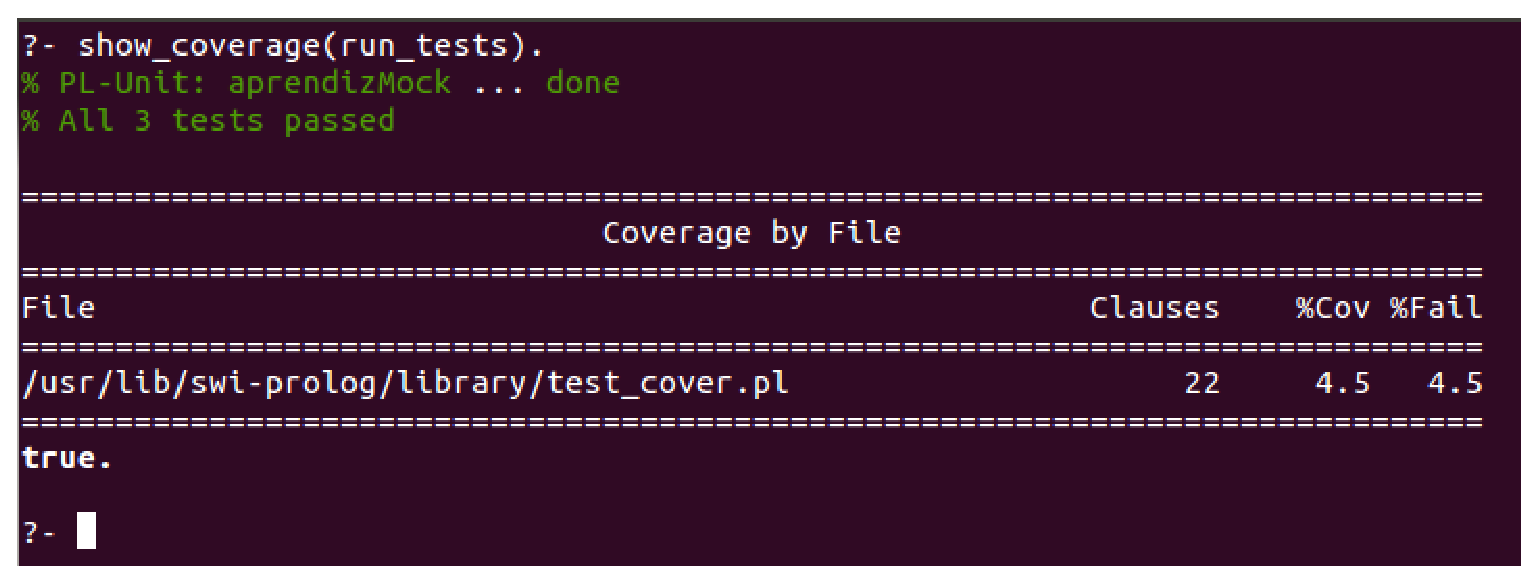
\includegraphics[width=0.9\textwidth]{figuras/prologTeste1}
\caption{Suíte de teste da base aprendiz.pl}
\label{prologTeste1}
\end{figure}

\begin{figure}[H]
\centering
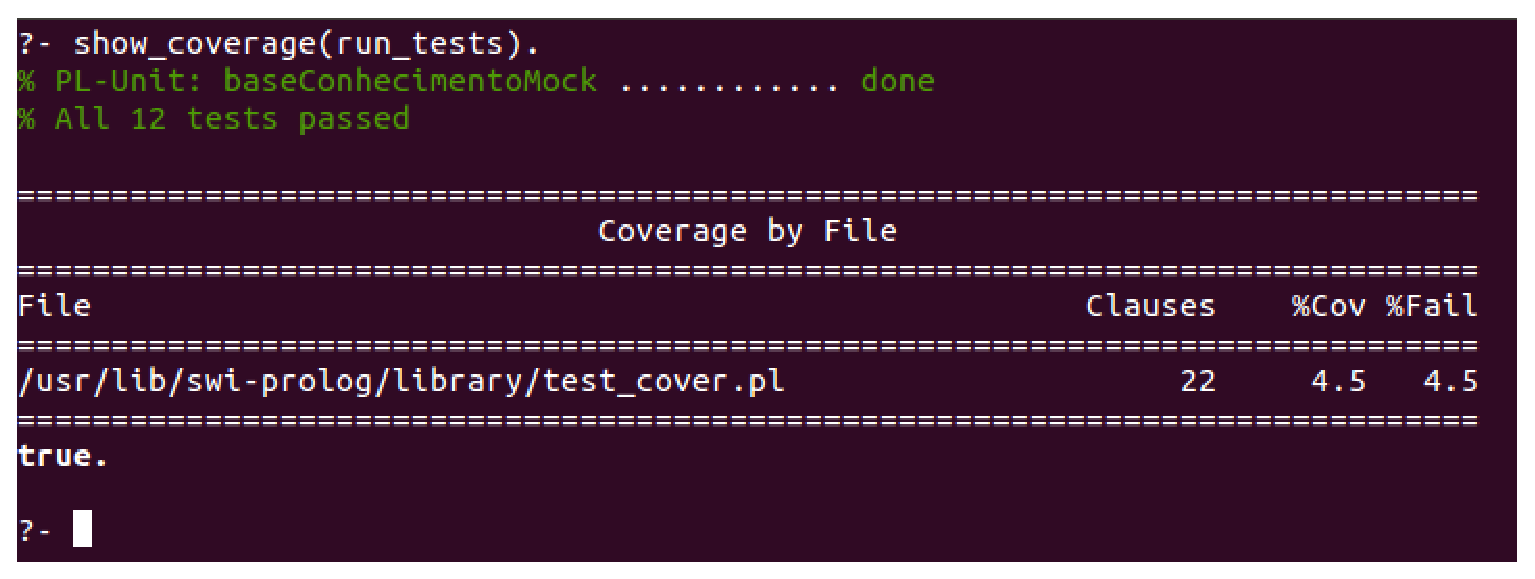
\includegraphics[width=0.9\textwidth]{figuras/prologTeste2}
\caption{Suíte de teste da base de conhecimento}
\label{prologTeste2}
\end{figure}

Os códigos referentes aos testes unitários em linguagem Prolog encontram-se no apêndice H.

\subsection{Componente Multiagentes}
Foram utilizados os frameworks Junit e Easy-mock para realização dos testes unitários na linguagem Java. Para obter a cobertura de código fonte, foi utilizada a ferramenta Eclemma. Obteve-se uma cobertura de código fonte de 84.8\% nos testes unitários, conforme pode ser visualizado na Figura \ref{eclemmaSMA}. 

\begin{figure}[H]
\centering
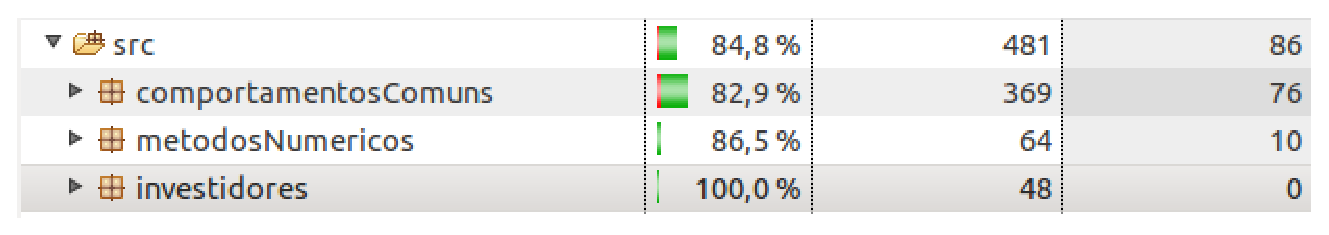
\includegraphics[width=0.9\textwidth]{figuras/eclemmaSMA}
\caption{Cobertura de Código dos pacotes do Componente Multiagentes}
\label{eclemmaSMA}
\end{figure}

O comportamento dos agentes são executados através dos métodos \textit{actions} e muitos  comportamentos precisavam de um tempo de até 6 (seis) segundos para serem executados. Devido a isso, os testes unitários quebraram, pois nenhum comportamento era executado a tempo. Para tentar solucionar esse problema, foram colocados delays para que desse tempo dos agentes se comunicarem. A execução dos testes demorou mais de 18 (dezoito) segundos conforme pode ser visualizado no  canto superior esquerdo da Figura \ref{eclemmaTodasClasses}. Apesar de todos os testes passarem pelo Junit e o Easy-mock com os delays, a ferramenta Eclemma não pegava a cobertura de código dos métodos \textit{actions} e devido a isso esses métodos foram ignorados no percentual de cobertura de código fonte.

\begin{figure}[H]
\centering
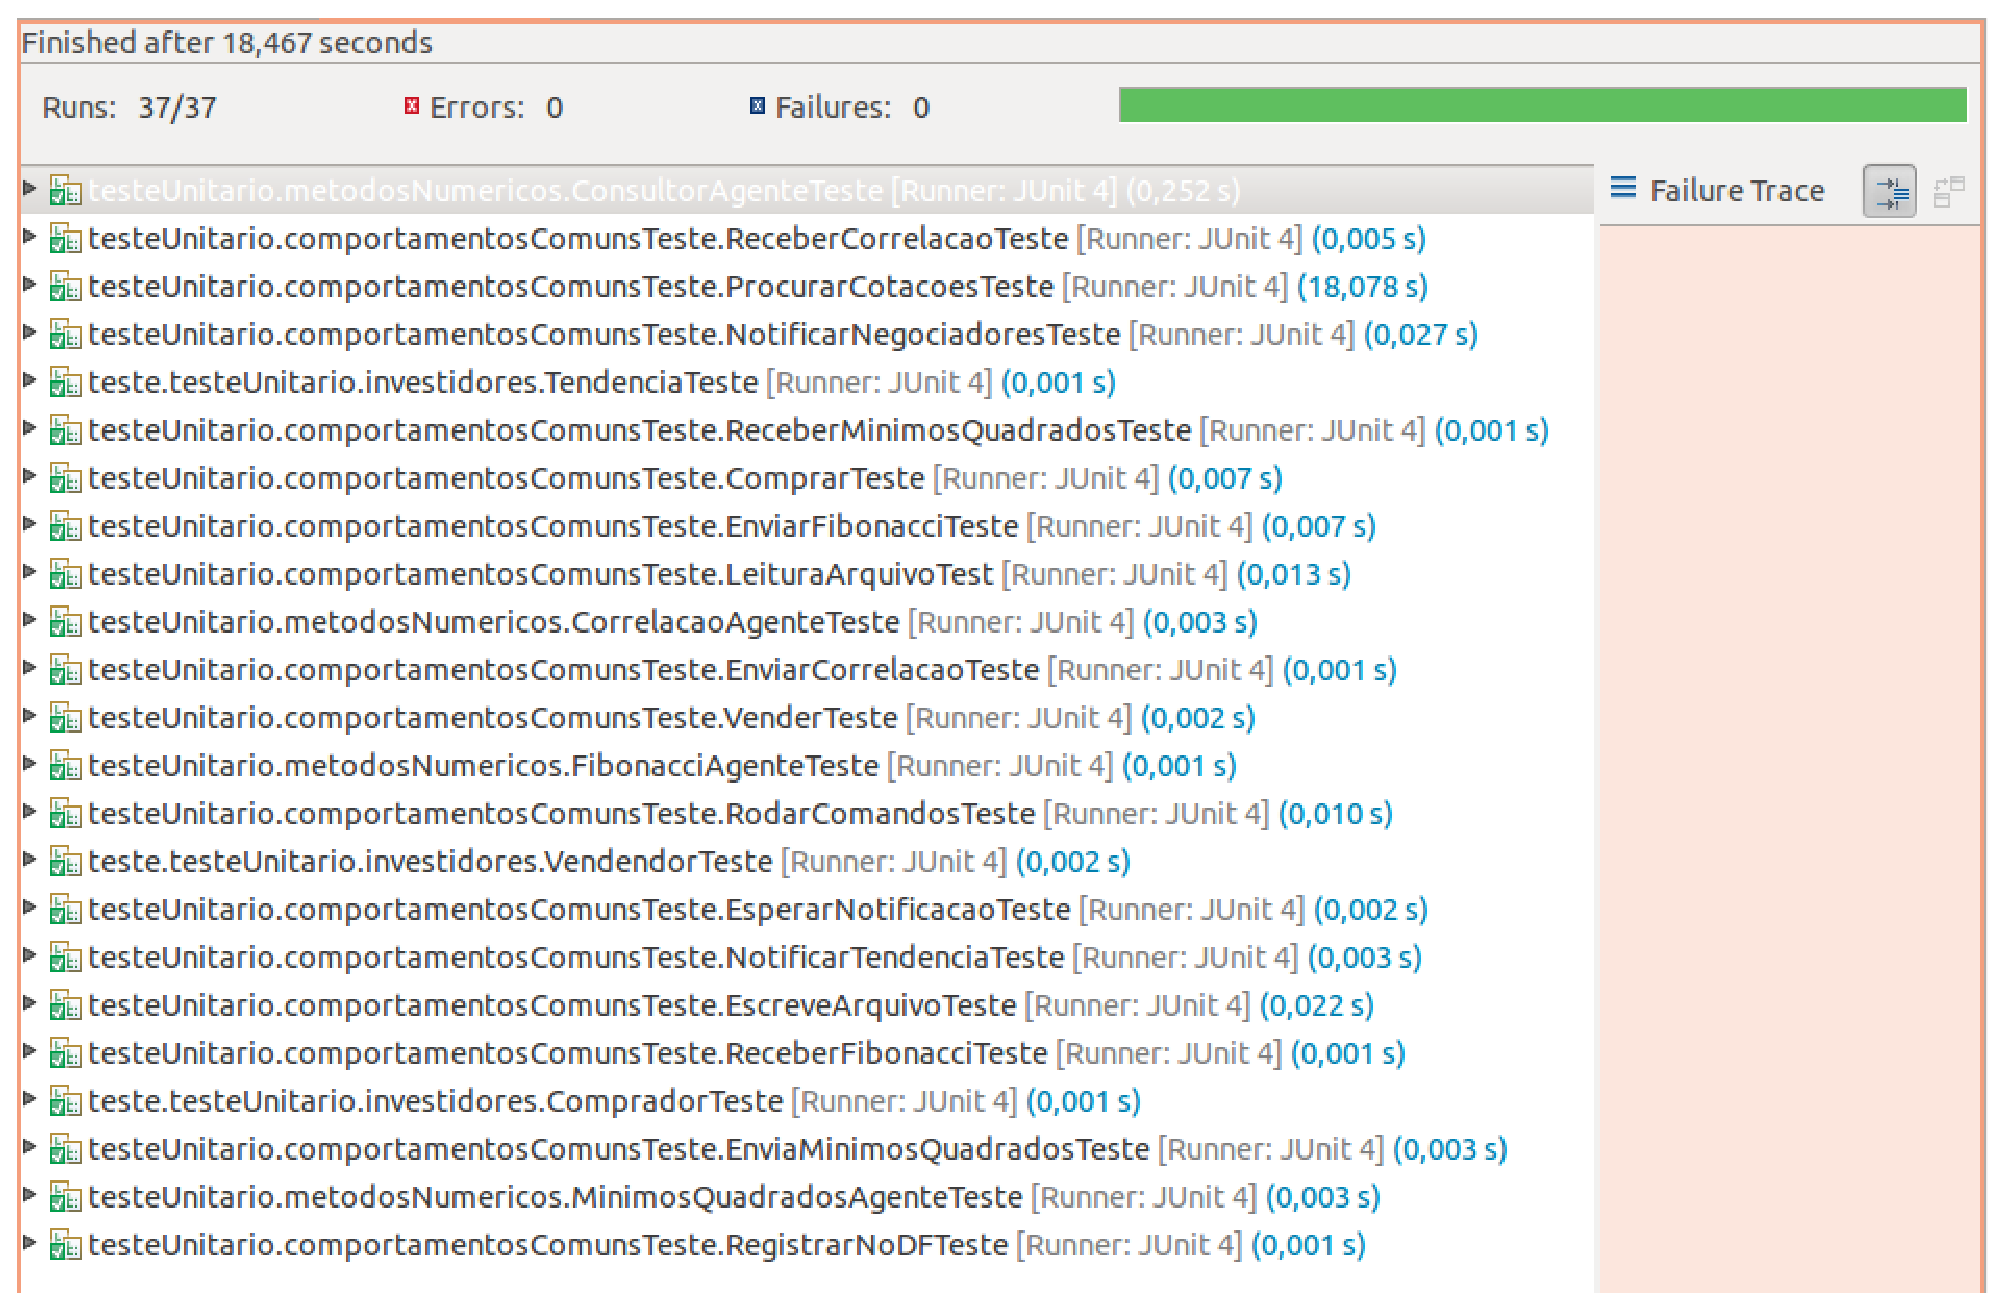
\includegraphics[width=0.9\textwidth]{figuras/eclemmaTodasClasses}
\caption{Suite de teste do Componente Multiagentes}
\label{eclemmaTodasClasses}
\end{figure}

As classes de teste mais significativas encontram-se no apêndice I.

\section{Análise estática de código fonte}
